\begin{table}[h]
	\centering

\begin{tabular}{ | c || r | r ||  l  || c || r | r | }
		\hline
		$p_\text{T} \text{ (GeV}/c)$ & Integral & Unsicherheit & \ & $p_\text{T} \text{ (GeV}/c)$ & Integral & Unsicherheit \\ \hline
		1,4 - 1,6 & 8183,77 \  & 248,36 \hspace{3mm}  & \ &  5,0 - 5,2 & 375,78 \ & 76,18 \hspace{3mm} \\ \hline
		1,6 - 1,8 & 12696,80 \ & 319,21 \hspace{3mm} & \ &  5,2 - 5,4 & 183,20 \ & 70,98 \hspace{3mm} \\ \hline
		1,8 - 2,0 & 14928,40 \ & 335,82 \hspace{3mm} & \ &  5,4 - 5,6 & 273,14 \ & 64,85 \hspace{3mm} \\ \hline
		2,0 - 2,2 & 13686,40 \ & 323,90 \hspace{3mm} & \ &  5,6 - 5,8 & 105,55 \ & 61,23 \hspace{3mm} \\ \hline
		2,2 - 2,4 & 10766,10 \ & 300,70 \hspace{3mm} & \ &  5,8 - 6,0 & 106,59 \ & 56,42 \hspace{3mm} \\ \hline
		2,4 - 2,6 & 9047,53 \  & 273,67 \hspace{3mm} & \ &  6,0 - 6,2 & 34,35 \  & 52,23 \hspace{3mm} \\ \hline
		2,6 - 2,8 & 6901,65 \  & 246,32 \hspace{3mm} & \ &  6,2 - 6,4 & 3,41 \   & 49,94 \hspace{3mm} \\ \hline
		2,8 - 3,0 & 5429,20 \  & 221,03 \hspace{3mm} & \ &  6,4 - 6,6 & 8,73 \   & 46,40 \hspace{3mm} \\ \hline
		3,0 - 3,2 & 4220,52 \  & 198,67 \hspace{3mm} & \ &  6,6 - 6,8 & -23,16 \ & 43,73 \hspace{3mm} \\ \hline
		3,2 - 3,4 & 3253,74 \ & 178,66 \hspace{3mm} & \ &  6,8 - 7,0 & -13,32 \ & 40,78 \hspace{3mm} \\ \hline
		3,4 - 3,6 & 2660,09 \ & 160,66 \hspace{3mm} & \ &  7,0 - 7,5 & -47,53 \ & 56,97 \hspace{3mm} \\ \hline
		3,6 - 3,8 & 1994,75 \ & 144,91 \hspace{3mm} & \ &  7,5 - 8,0 & -35,33 \ & 49,50 \hspace{3mm} \\ \hline
		3,8 - 4,0 & 1537,27 \ & 130,91 \hspace{3mm} & \ &  8,0 - 8,5 & -79,79 \ & 42,67 \hspace{3mm} \\ \hline
		4,0 - 4,2 & 1411,16 \ & 118,39 \hspace{3mm} & \ &  8,5 - 9,0 & -85,09 \ & 39,43 \hspace{3mm} \\ \hline
		4,2 - 4,4 & 852,25 \  & 108,17 \hspace{3mm} & \ &  9,0 - 9,5 & -39,02 \ & 35,48 \hspace{3mm} \\ \hline
		4,4 - 4,6 & 817,07 \  & 99,02 \hspace{3mm} &  \ &  \ 9,5 - 10,0 & -32,65 \ & 31,98 \hspace{3mm} \\ \hline
		4,6 - 4,8 & 590,26 \  & 89,73 \hspace{3mm} &  \ &  10,0 - 12,0 & -288,32 \ & 50,04 \hspace{3mm} \\ \hline
		4,8 - 5,0 & 460,15 \  & 82,49 \hspace{3mm} &  \ & \   & \  & \  \\ \hline
	
\end{tabular}
	
\caption{Integral und Unsicherheit der Templates des korrelierten Untergrunds für die verschiedenen $p_\text{T}$-Intervalle.}
\label{tab:IntAndError}
\end{table}
\clearpage

\begin{figure*}[t]
\centering
\begin{multicols}{2}
    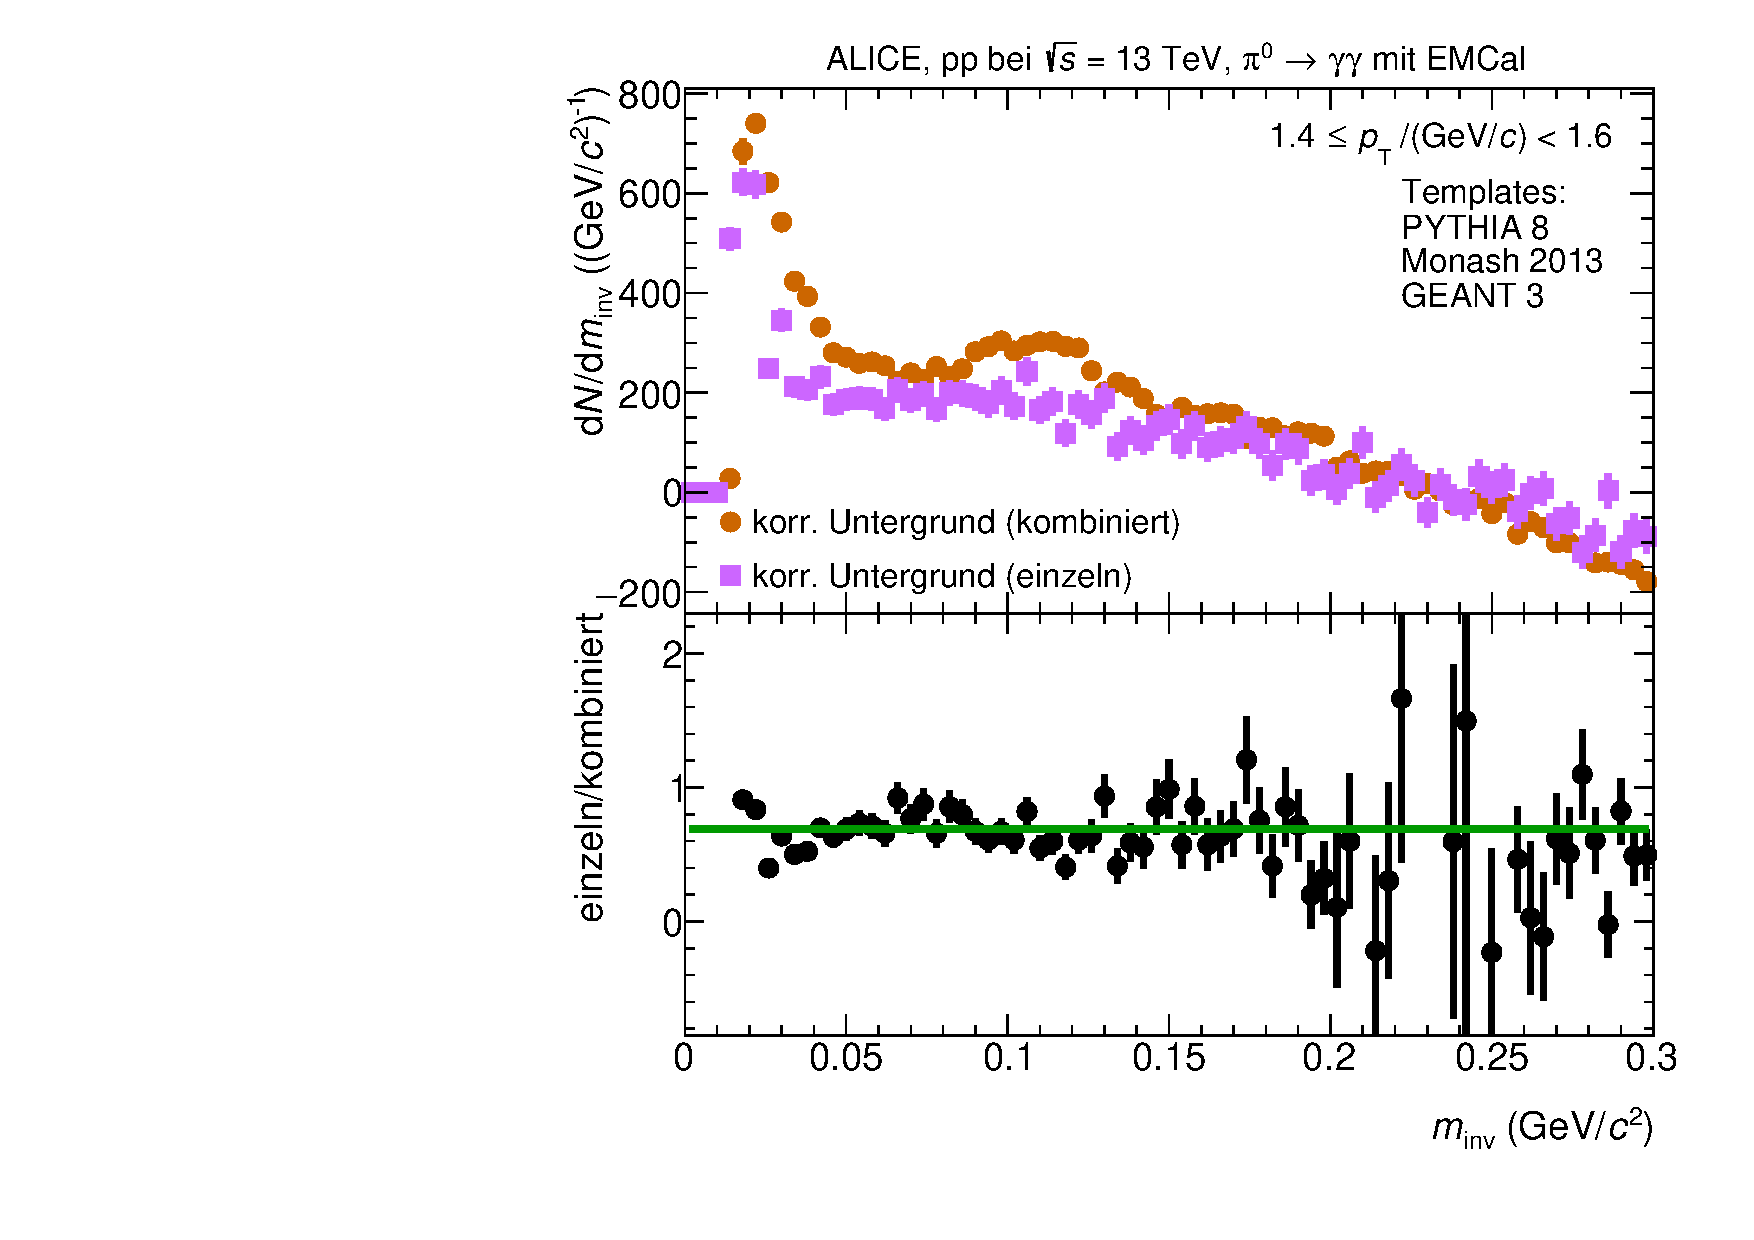
\includegraphics[width=.65\linewidth]{Anhang/BackgroundWithRatio01_Data_2016.pdf}\par 
    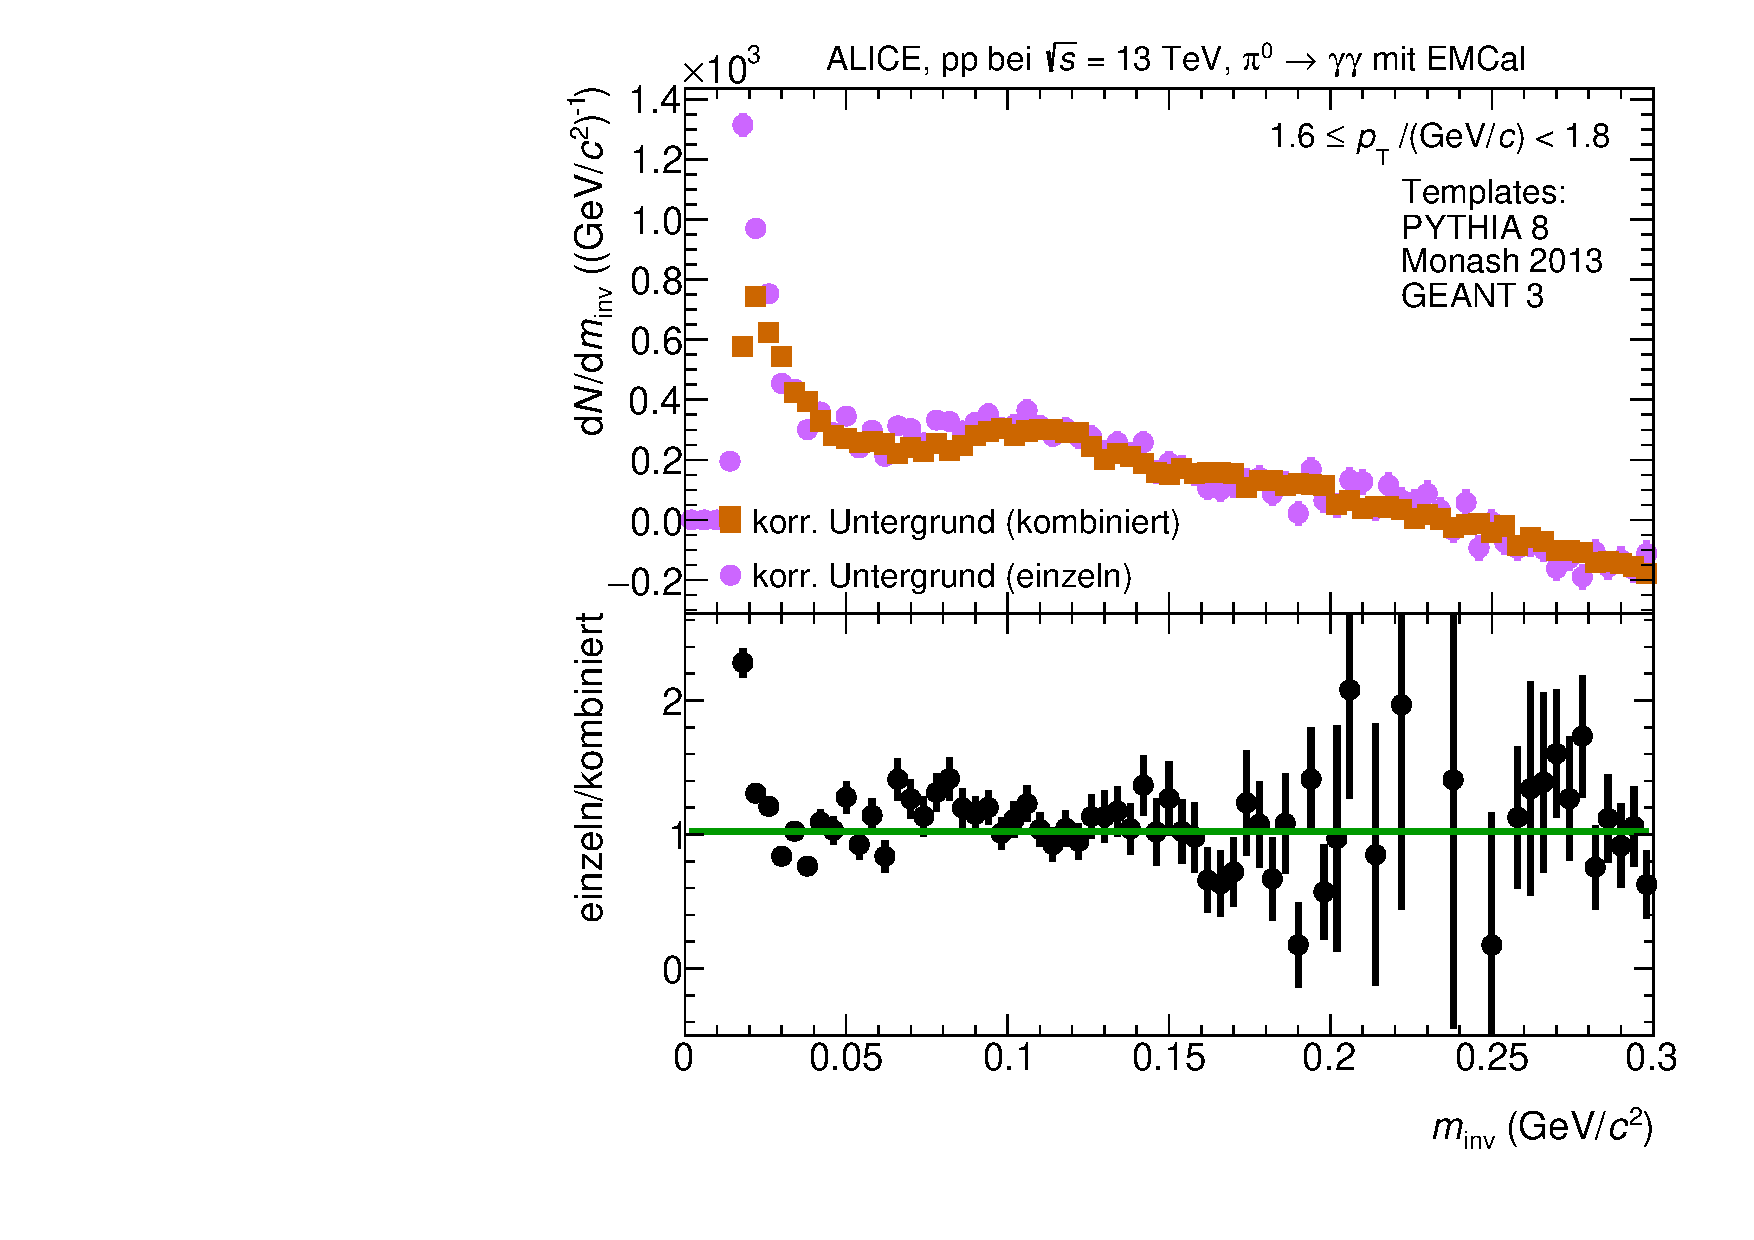
\includegraphics[width=.65\linewidth]{Anhang/BackgroundWithRatio02_Data_2016.pdf}\par 
\end{multicols}
\begin{multicols}{2}
    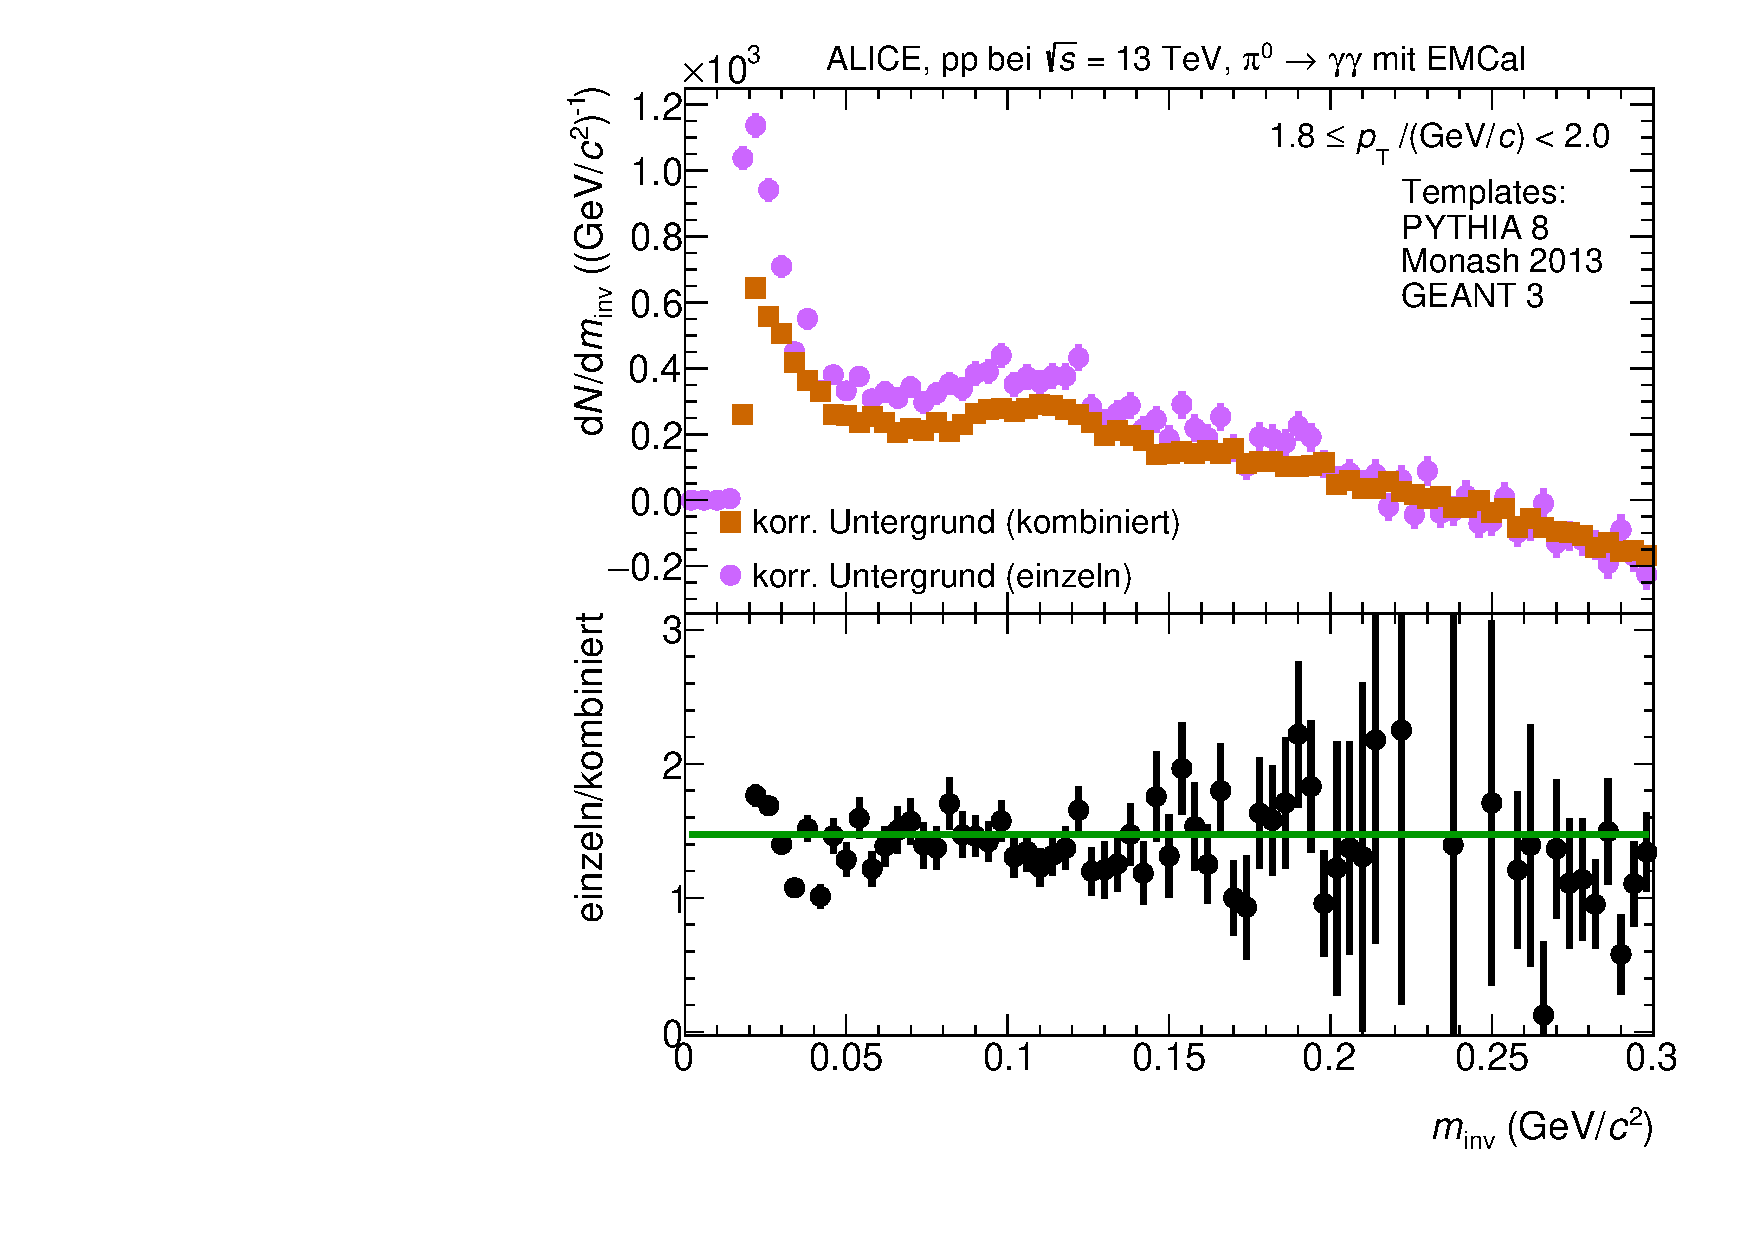
\includegraphics[width=.65\linewidth]{Anhang/BackgroundWithRatio03_Data_2016.pdf}\par
    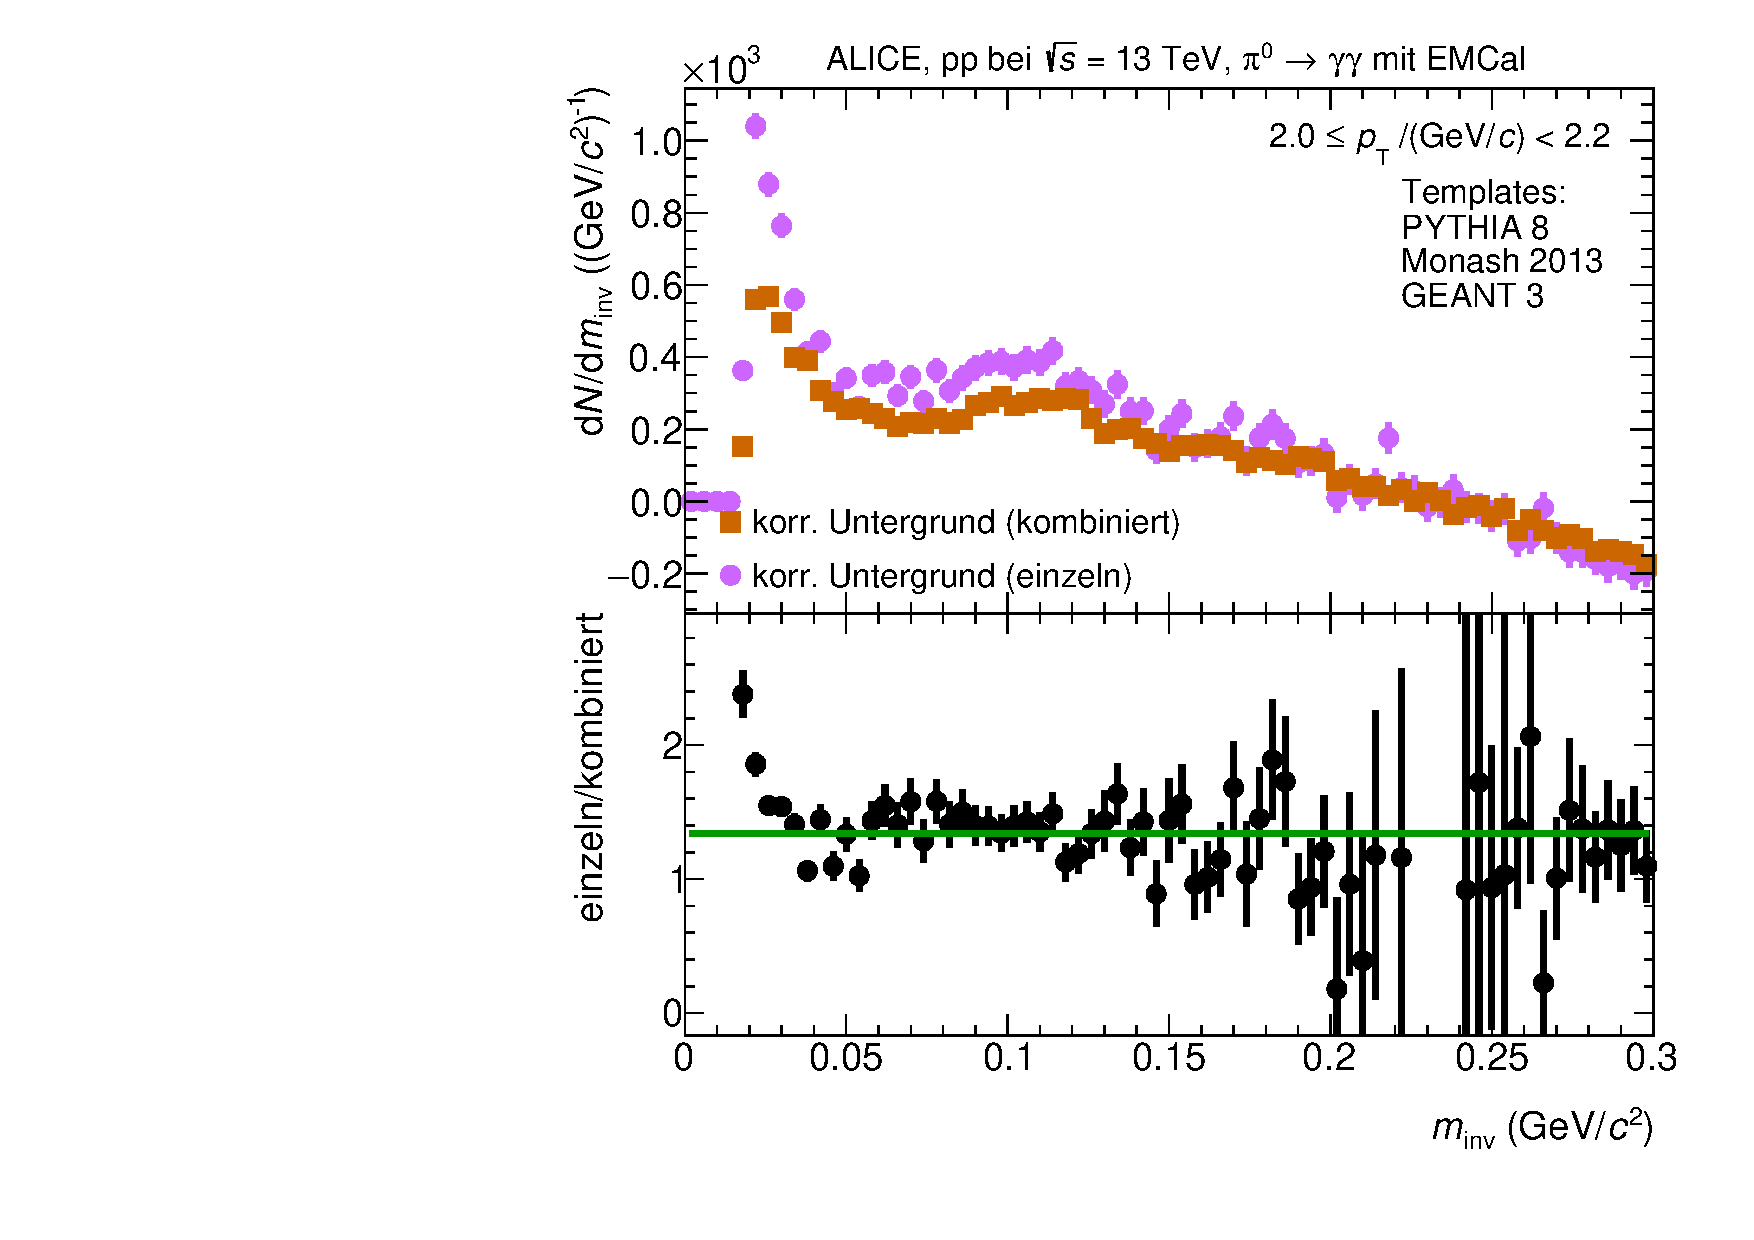
\includegraphics[width=.65\linewidth]{Anhang/BackgroundWithRatio04_Data_2016.pdf}\par
\end{multicols}
\begin{multicols}{2}
    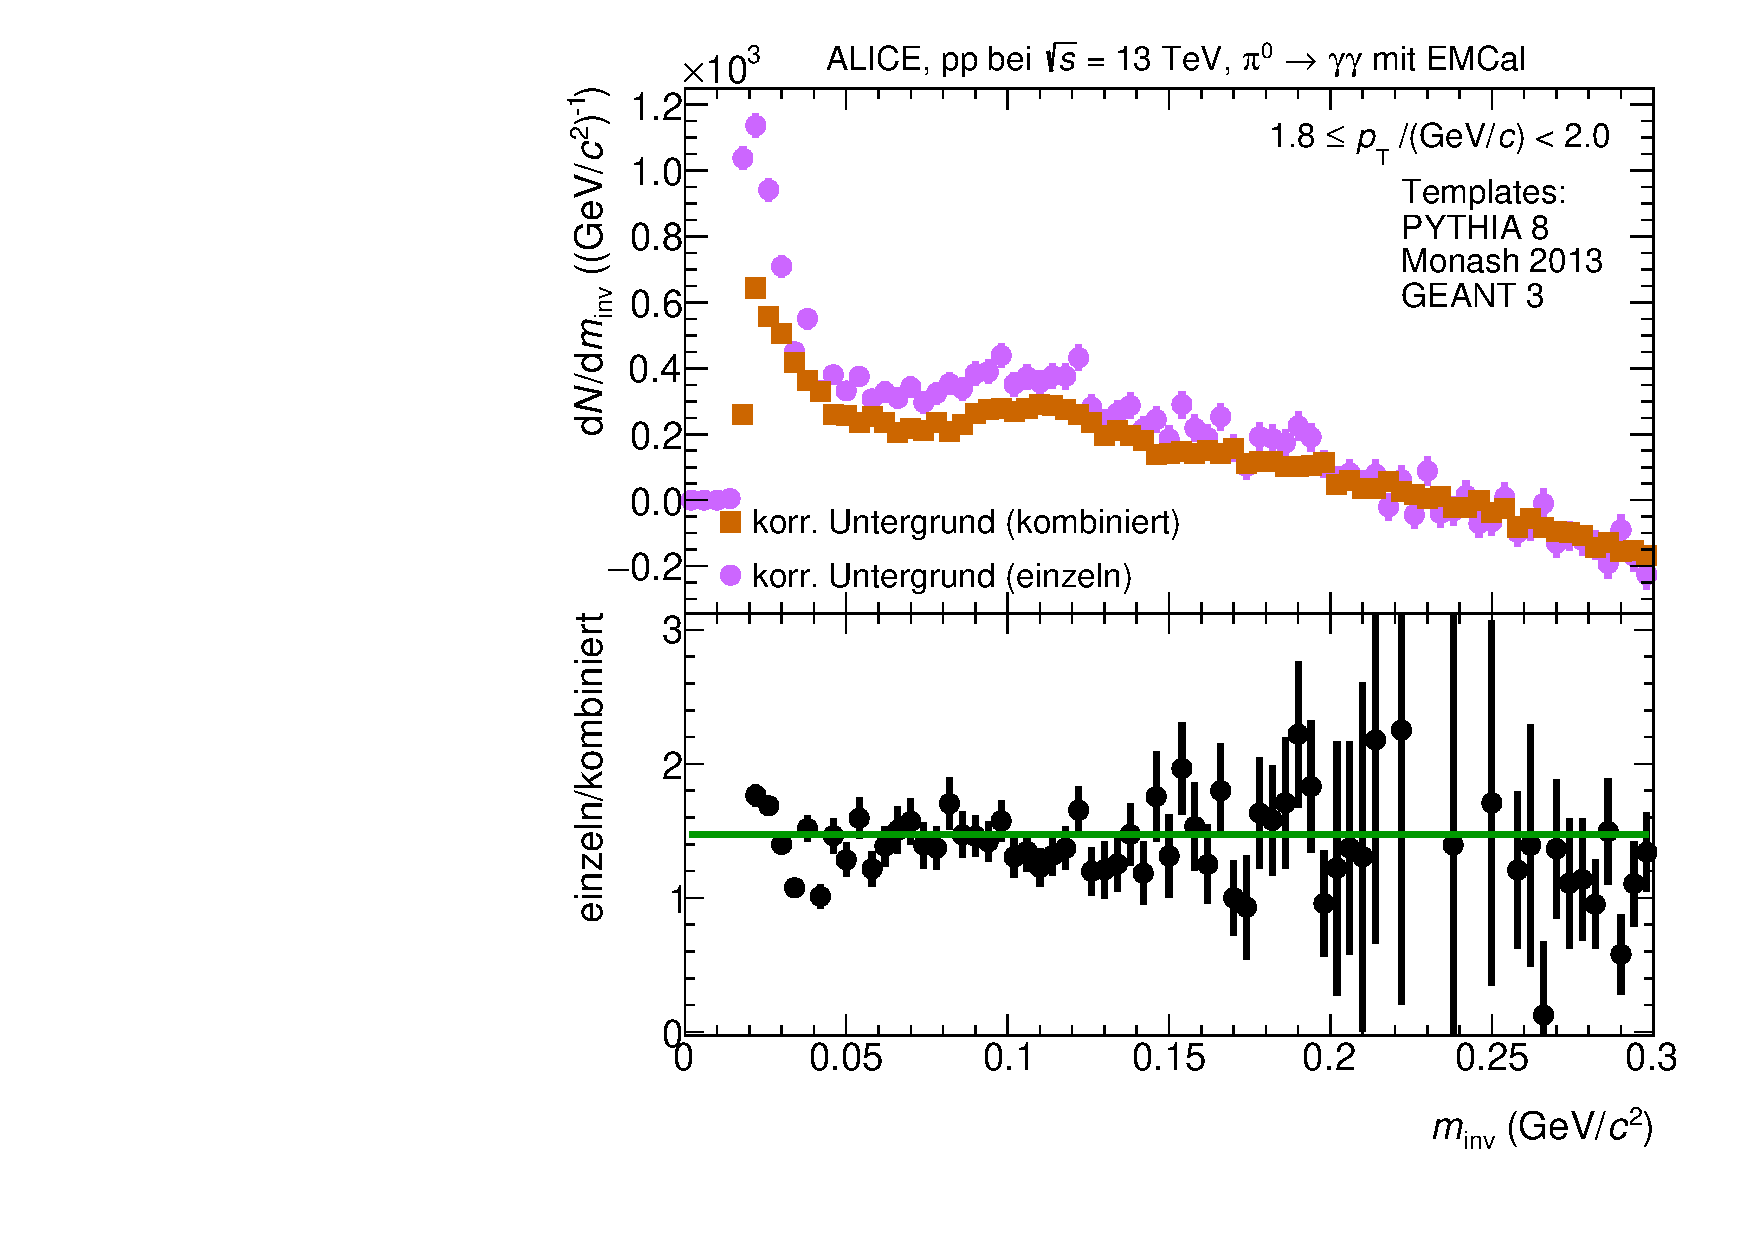
\includegraphics[width=.65\linewidth]{Anhang/BackgroundWithRatio03_Data_2016.pdf}\par
    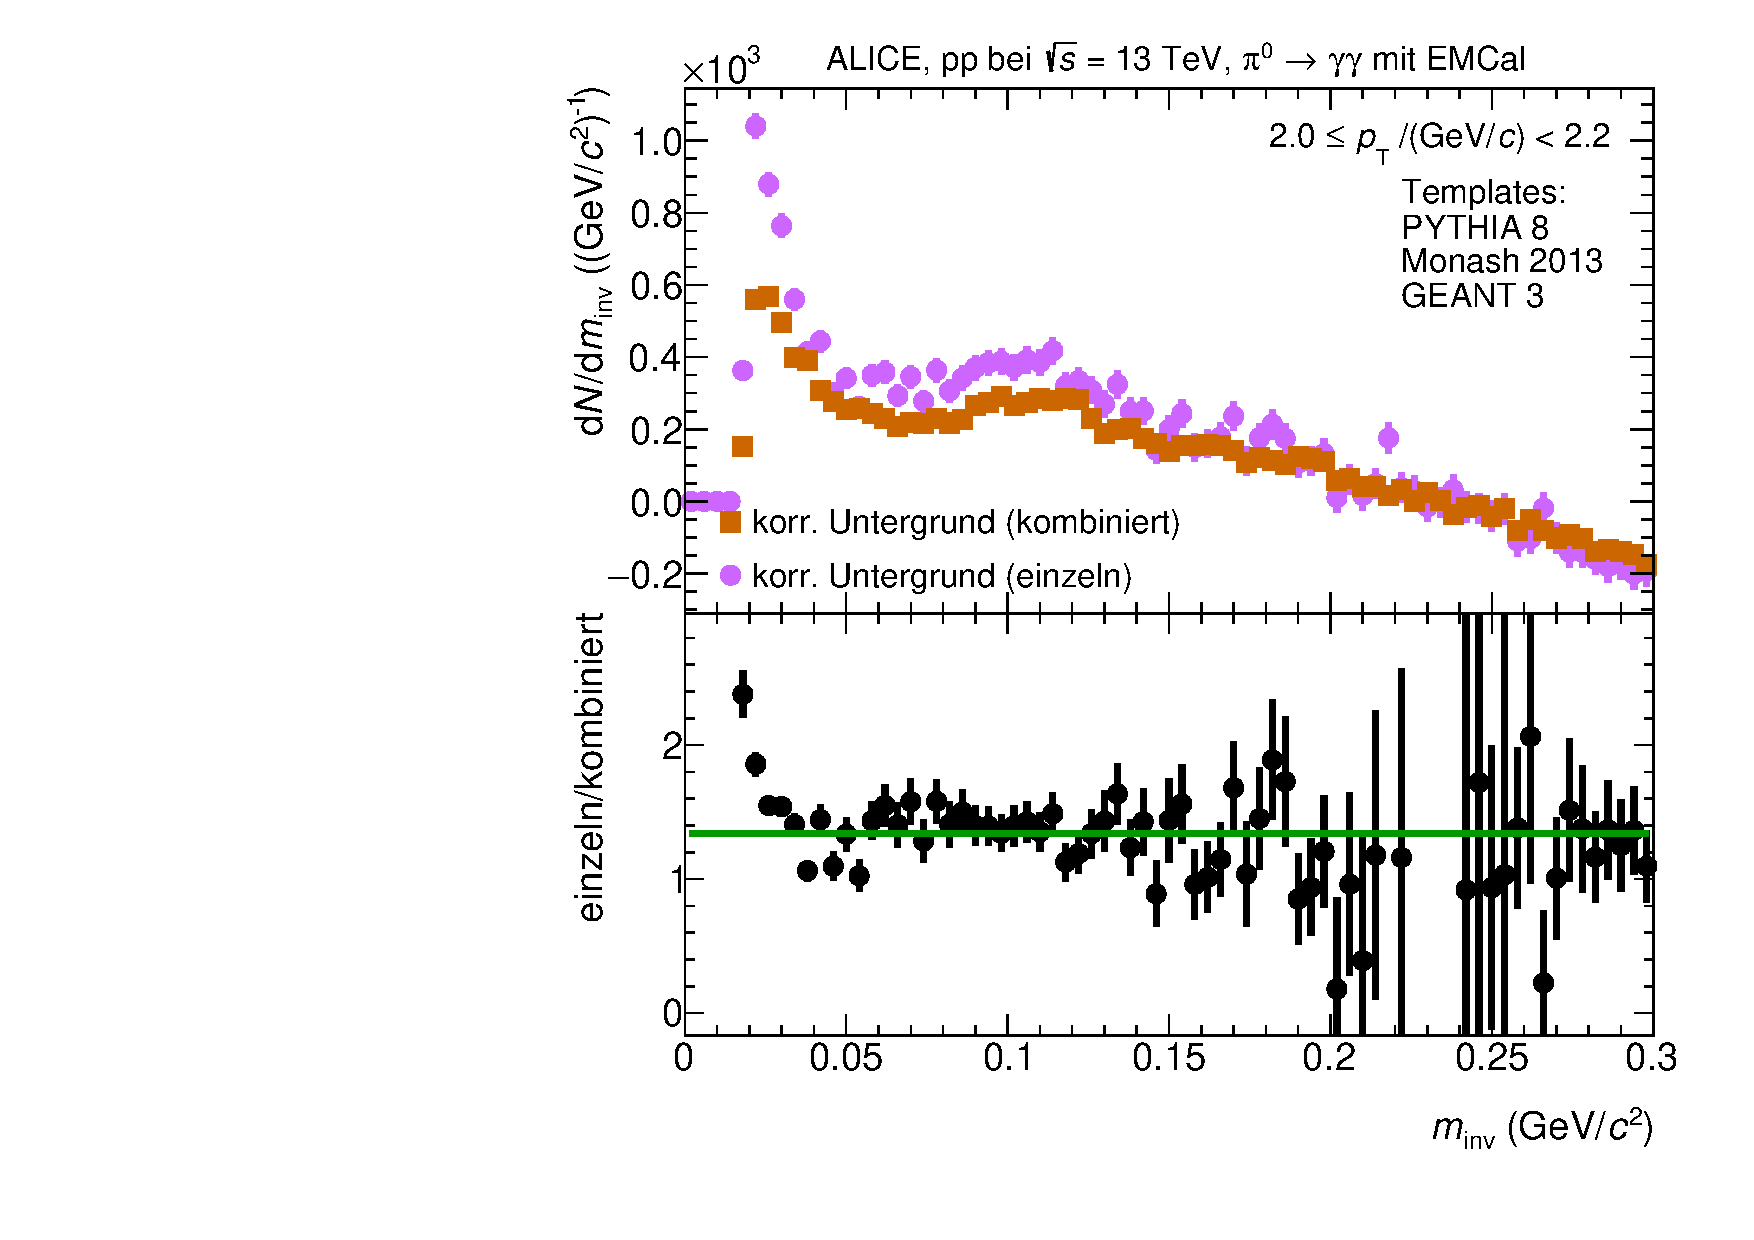
\includegraphics[width=.65\linewidth]{Anhang/BackgroundWithRatio04_Data_2016.pdf}\par
\end{multicols}
\begin{multicols}{2}
    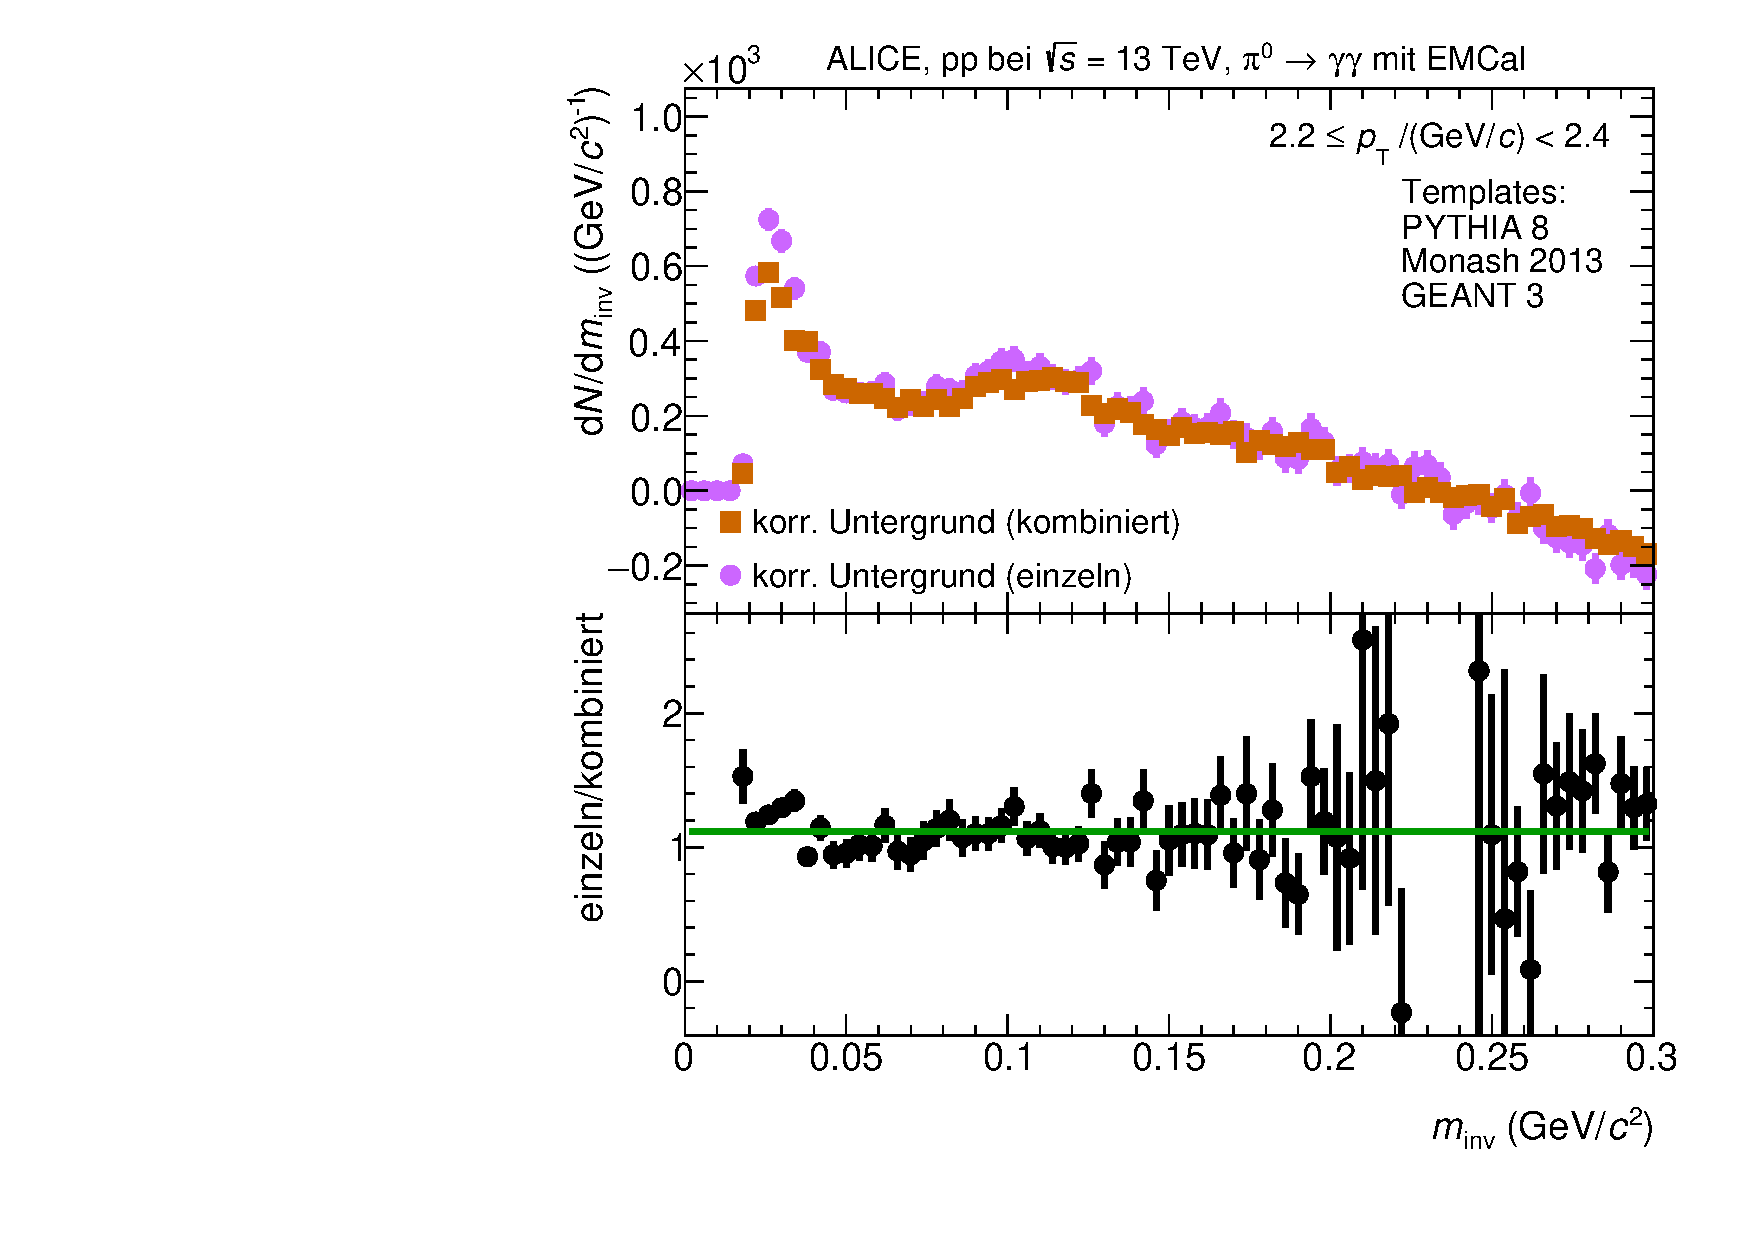
\includegraphics[width=.65\linewidth]{Anhang/BackgroundWithRatio05_Data_2016.pdf}\par
    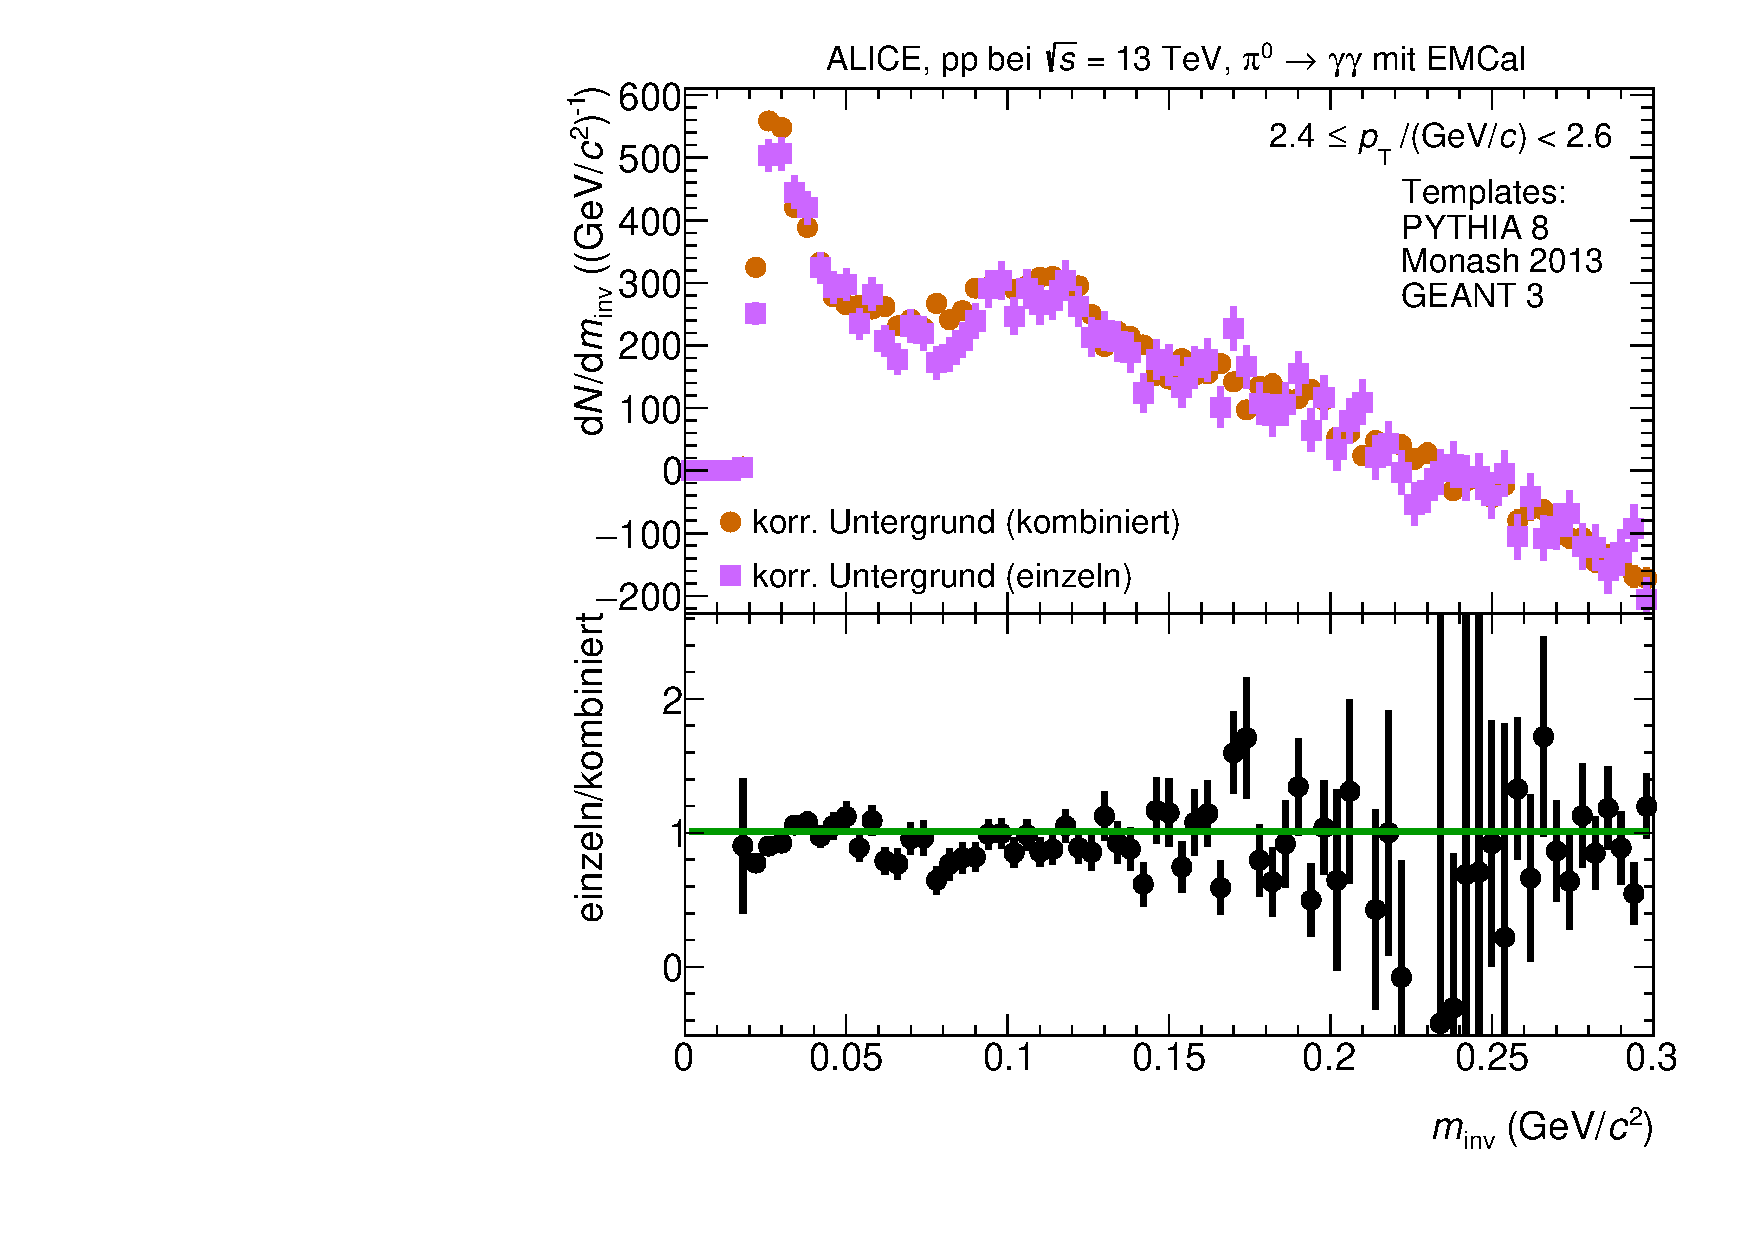
\includegraphics[width=.65\linewidth]{Anhang/BackgroundWithRatio06_Data_2016.pdf}\par
\end{multicols}
\end{figure*}
\clearpage

\begin{figure*}[t]
\centering
\begin{multicols}{2}
    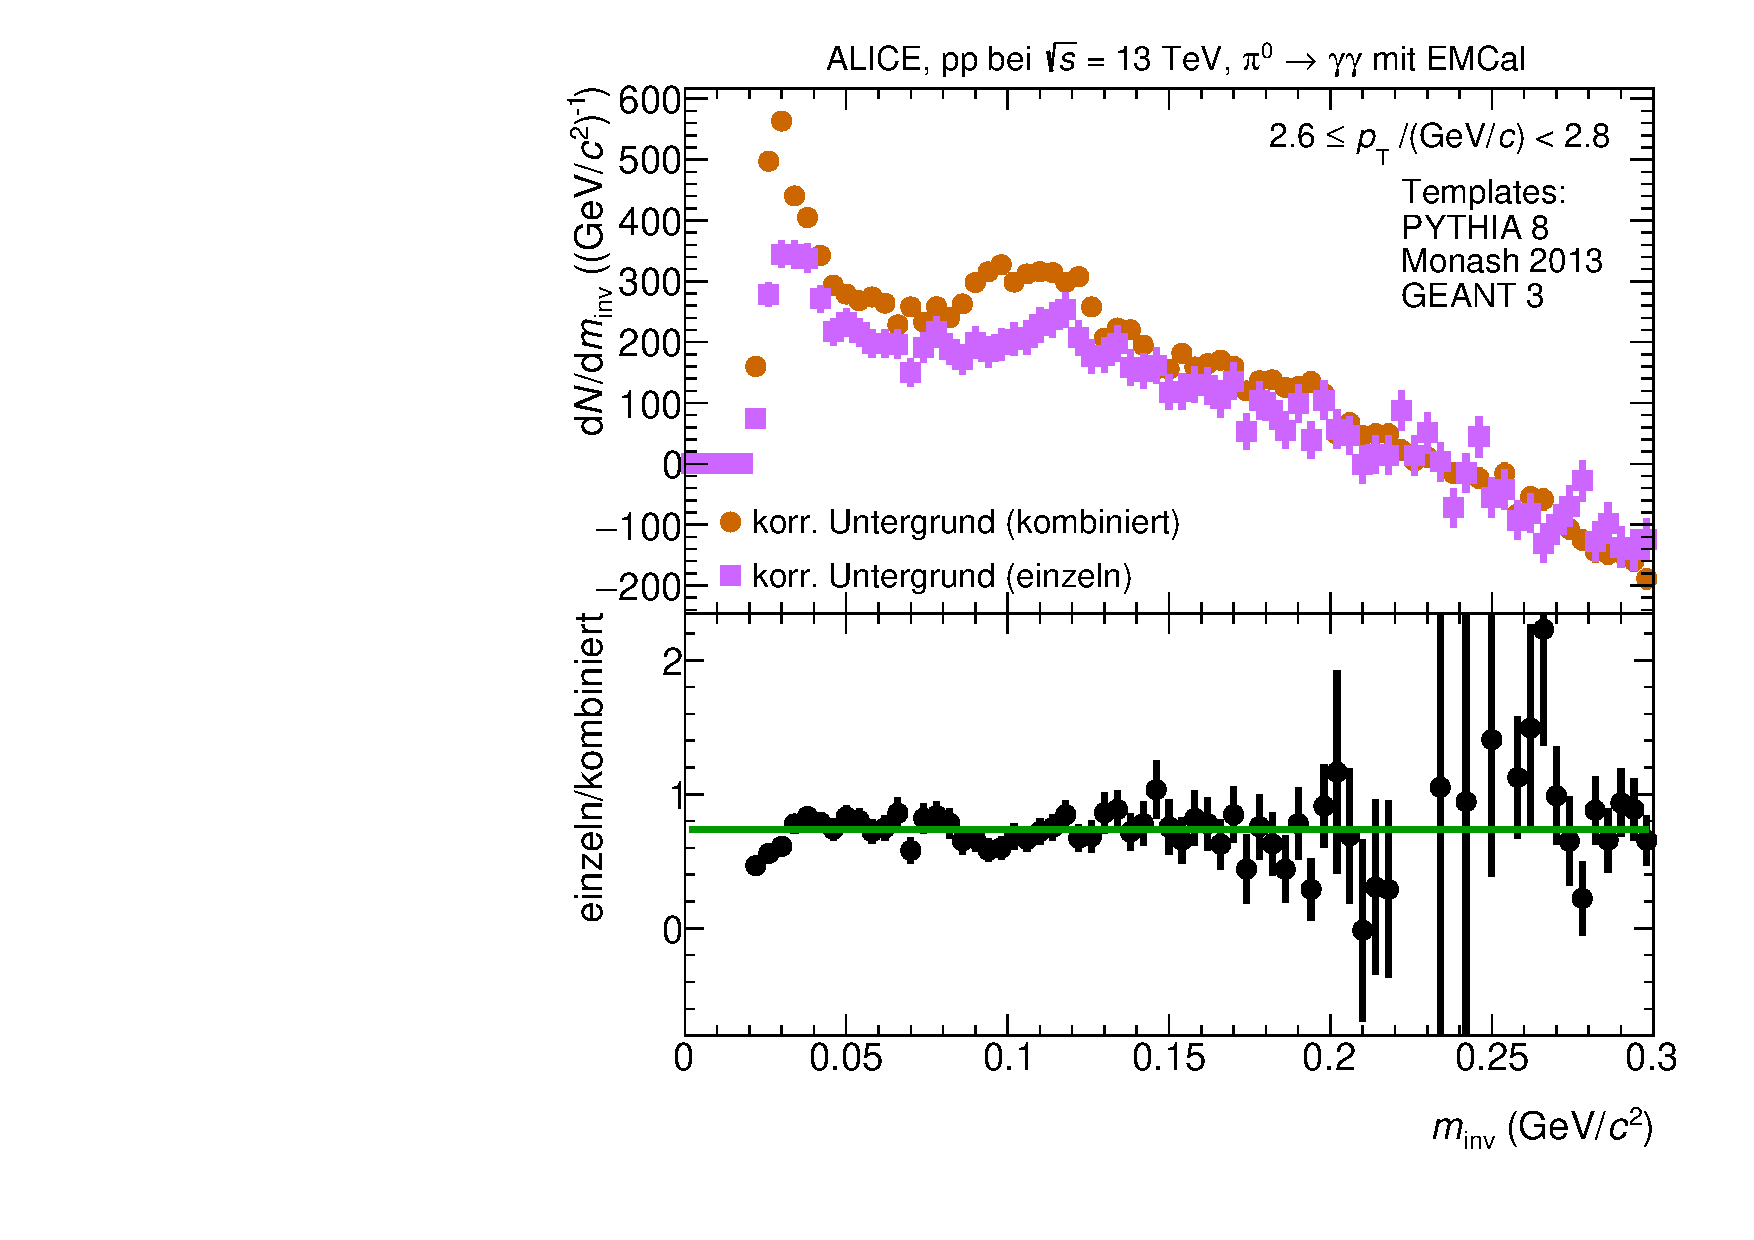
\includegraphics[width=.65\linewidth]{Anhang/BackgroundWithRatio07_Data_2016.pdf}\par 
    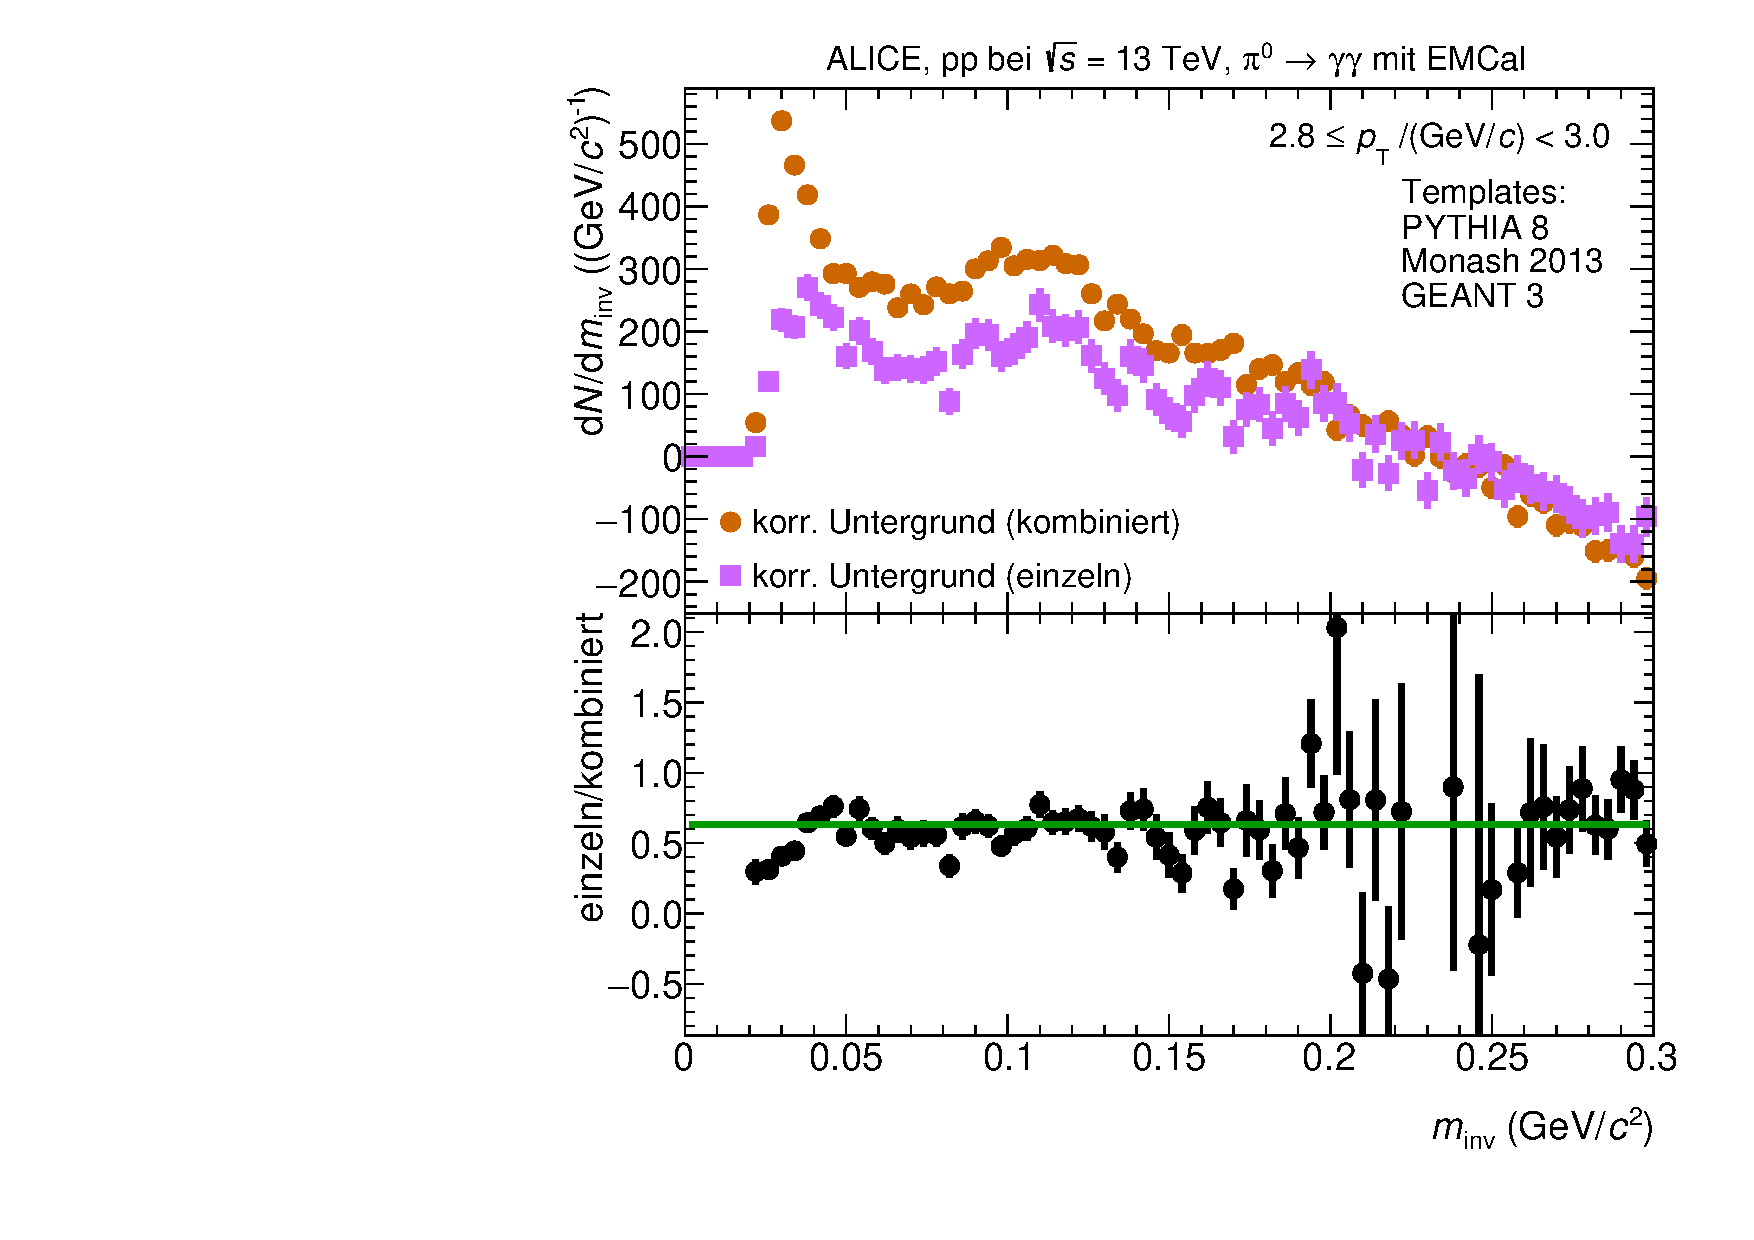
\includegraphics[width=.65\linewidth]{Anhang/BackgroundWithRatio08_Data_2016.pdf}\par 
\end{multicols}
\begin{multicols}{2}
    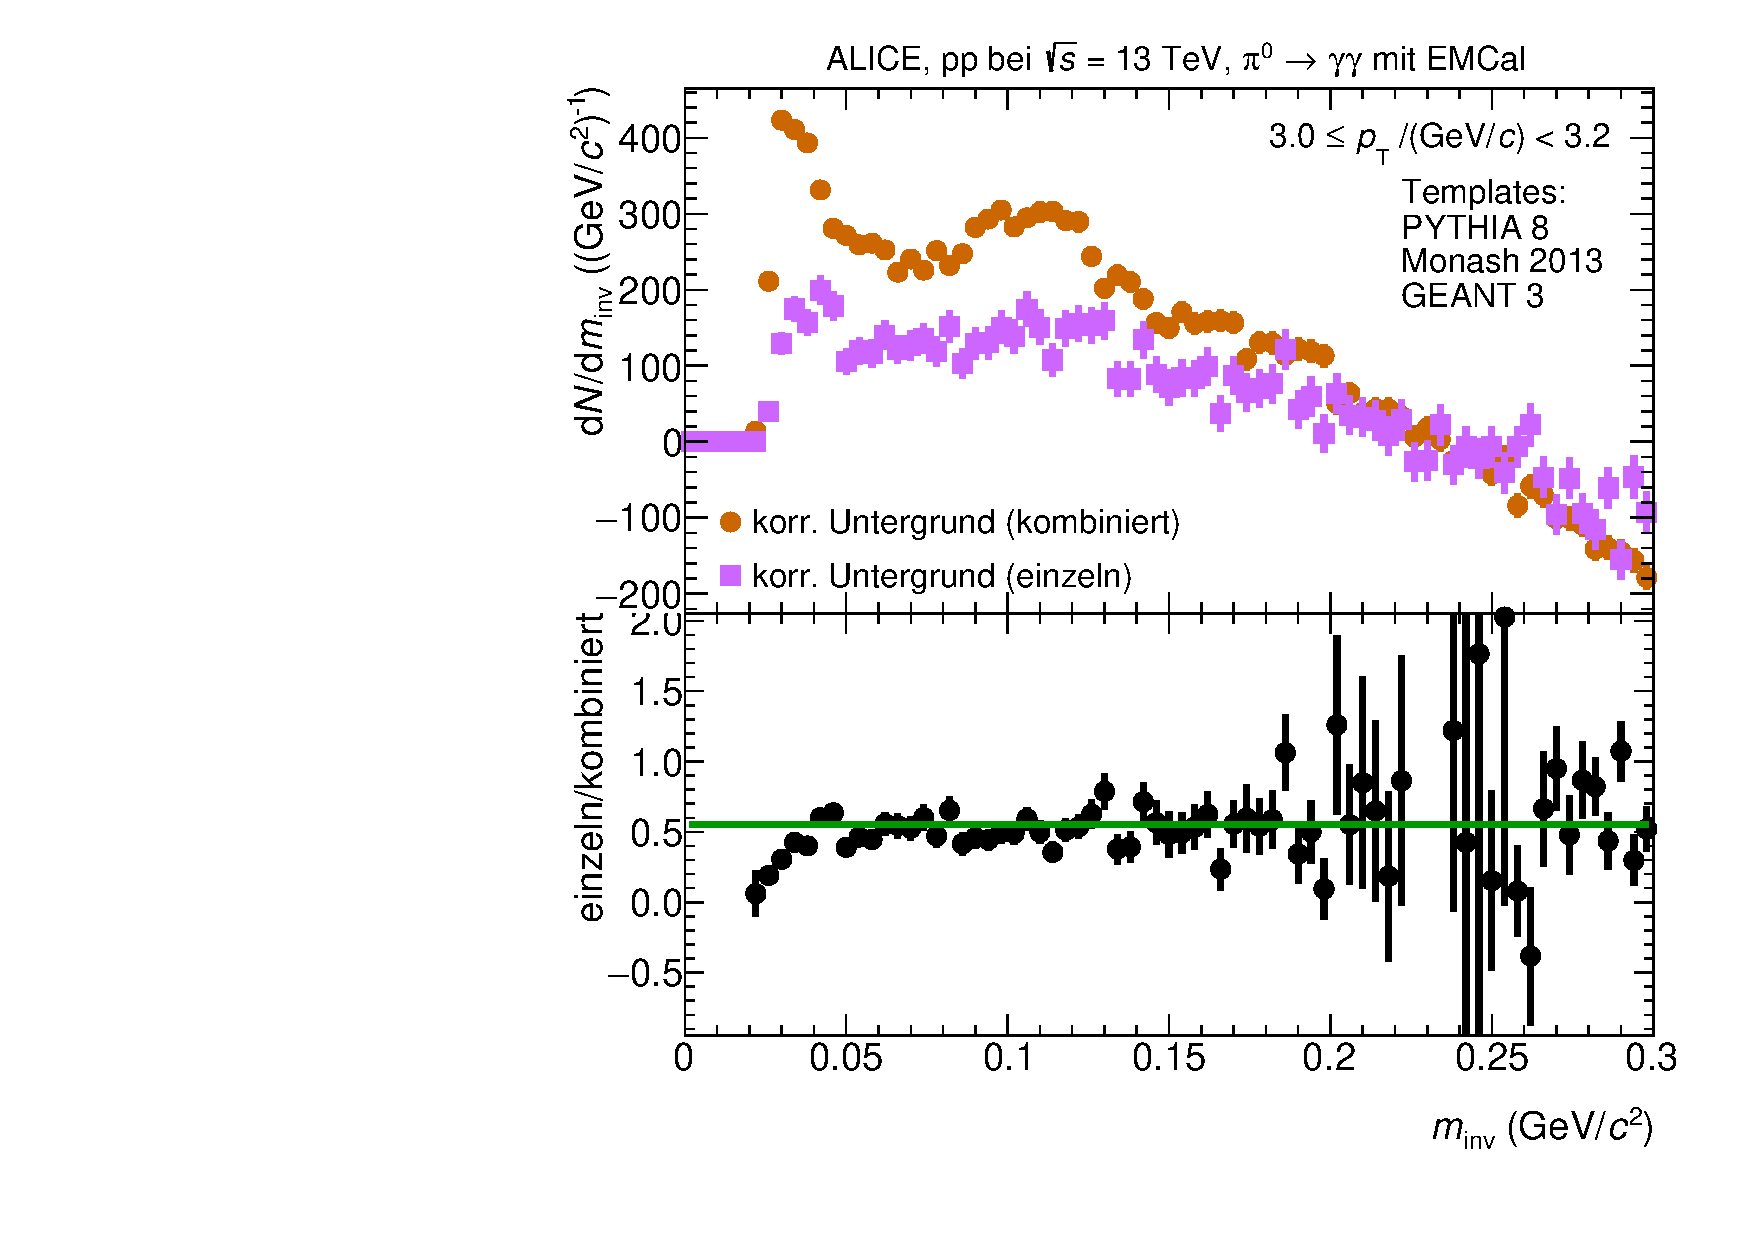
\includegraphics[width=.65\linewidth]{Anhang/BackgroundWithRatio09_Data_2016.pdf}\par
    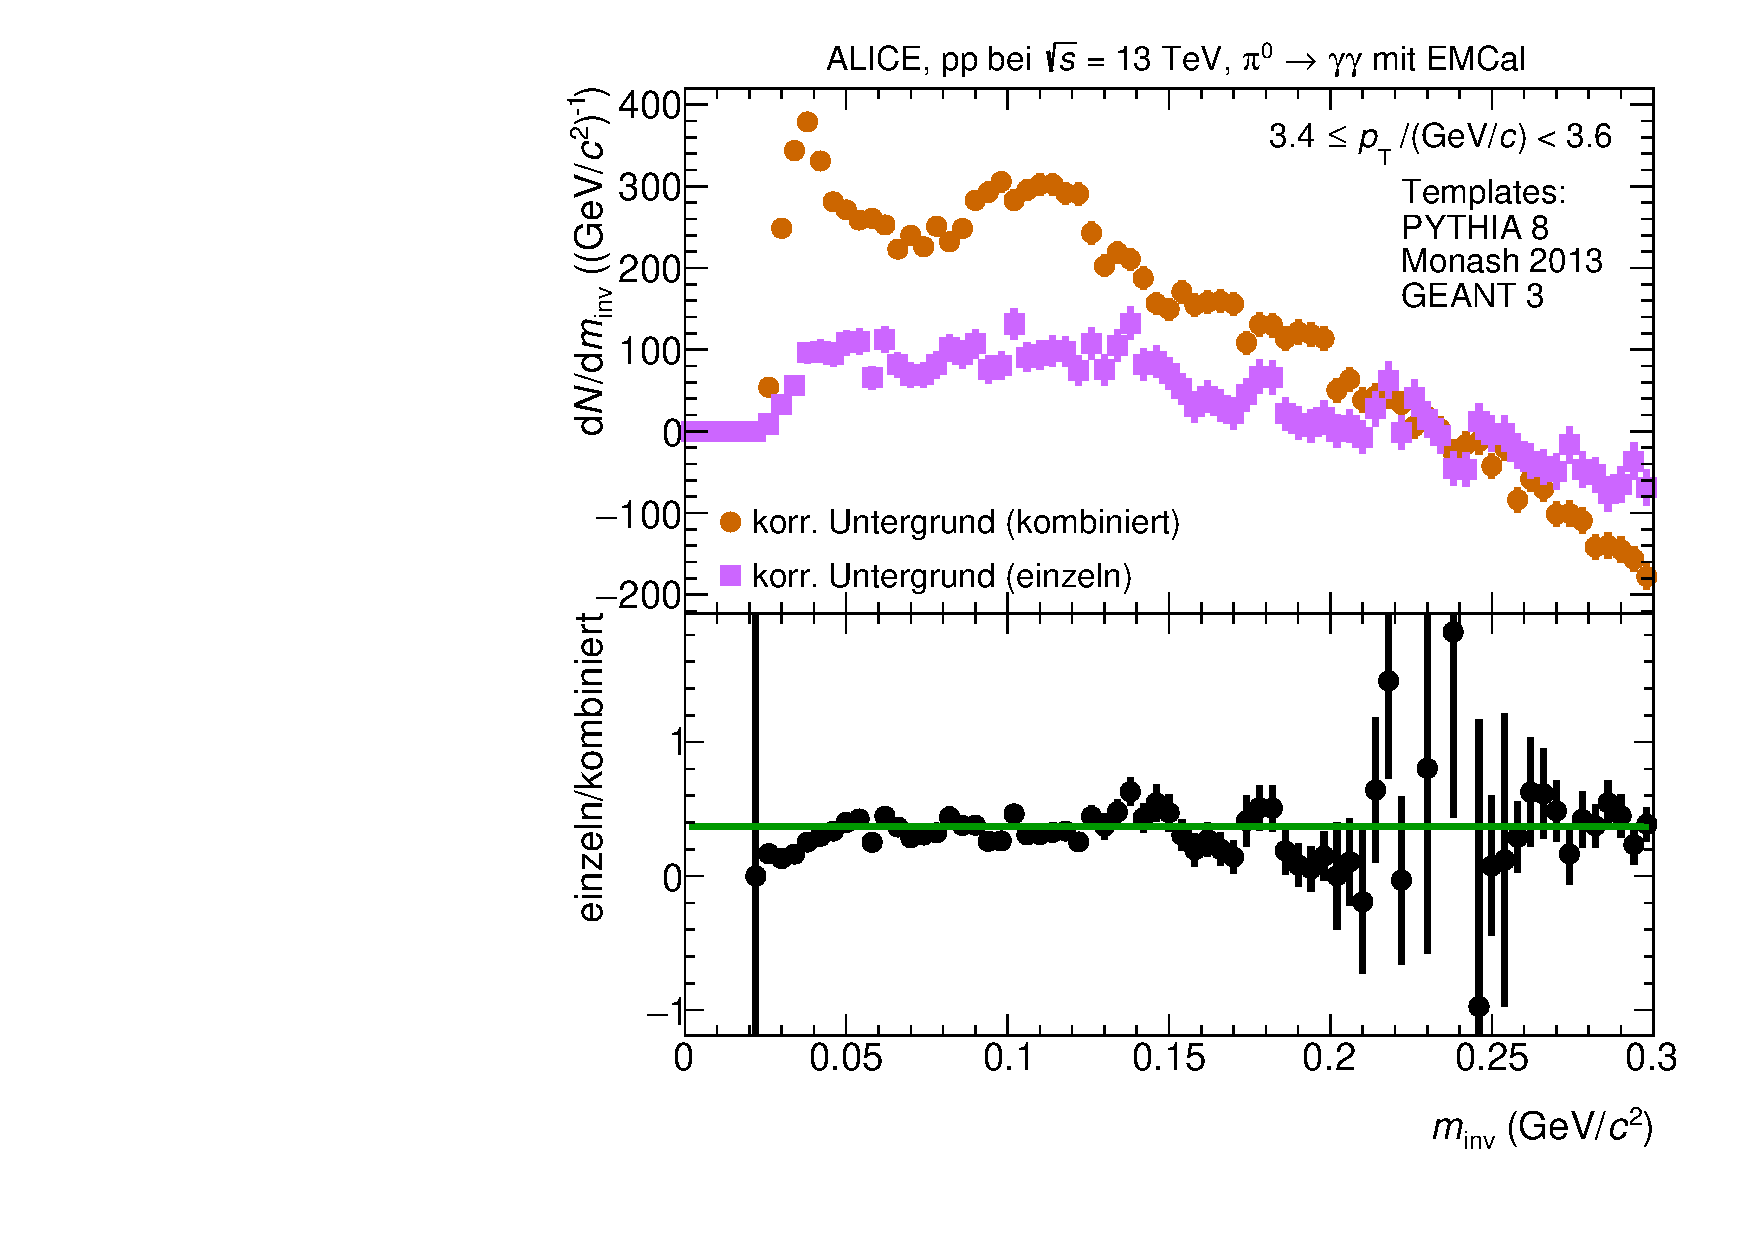
\includegraphics[width=.65\linewidth]{Anhang/BackgroundWithRatio11_Data_2016.pdf}\par
\end{multicols}
\begin{multicols}{2}
    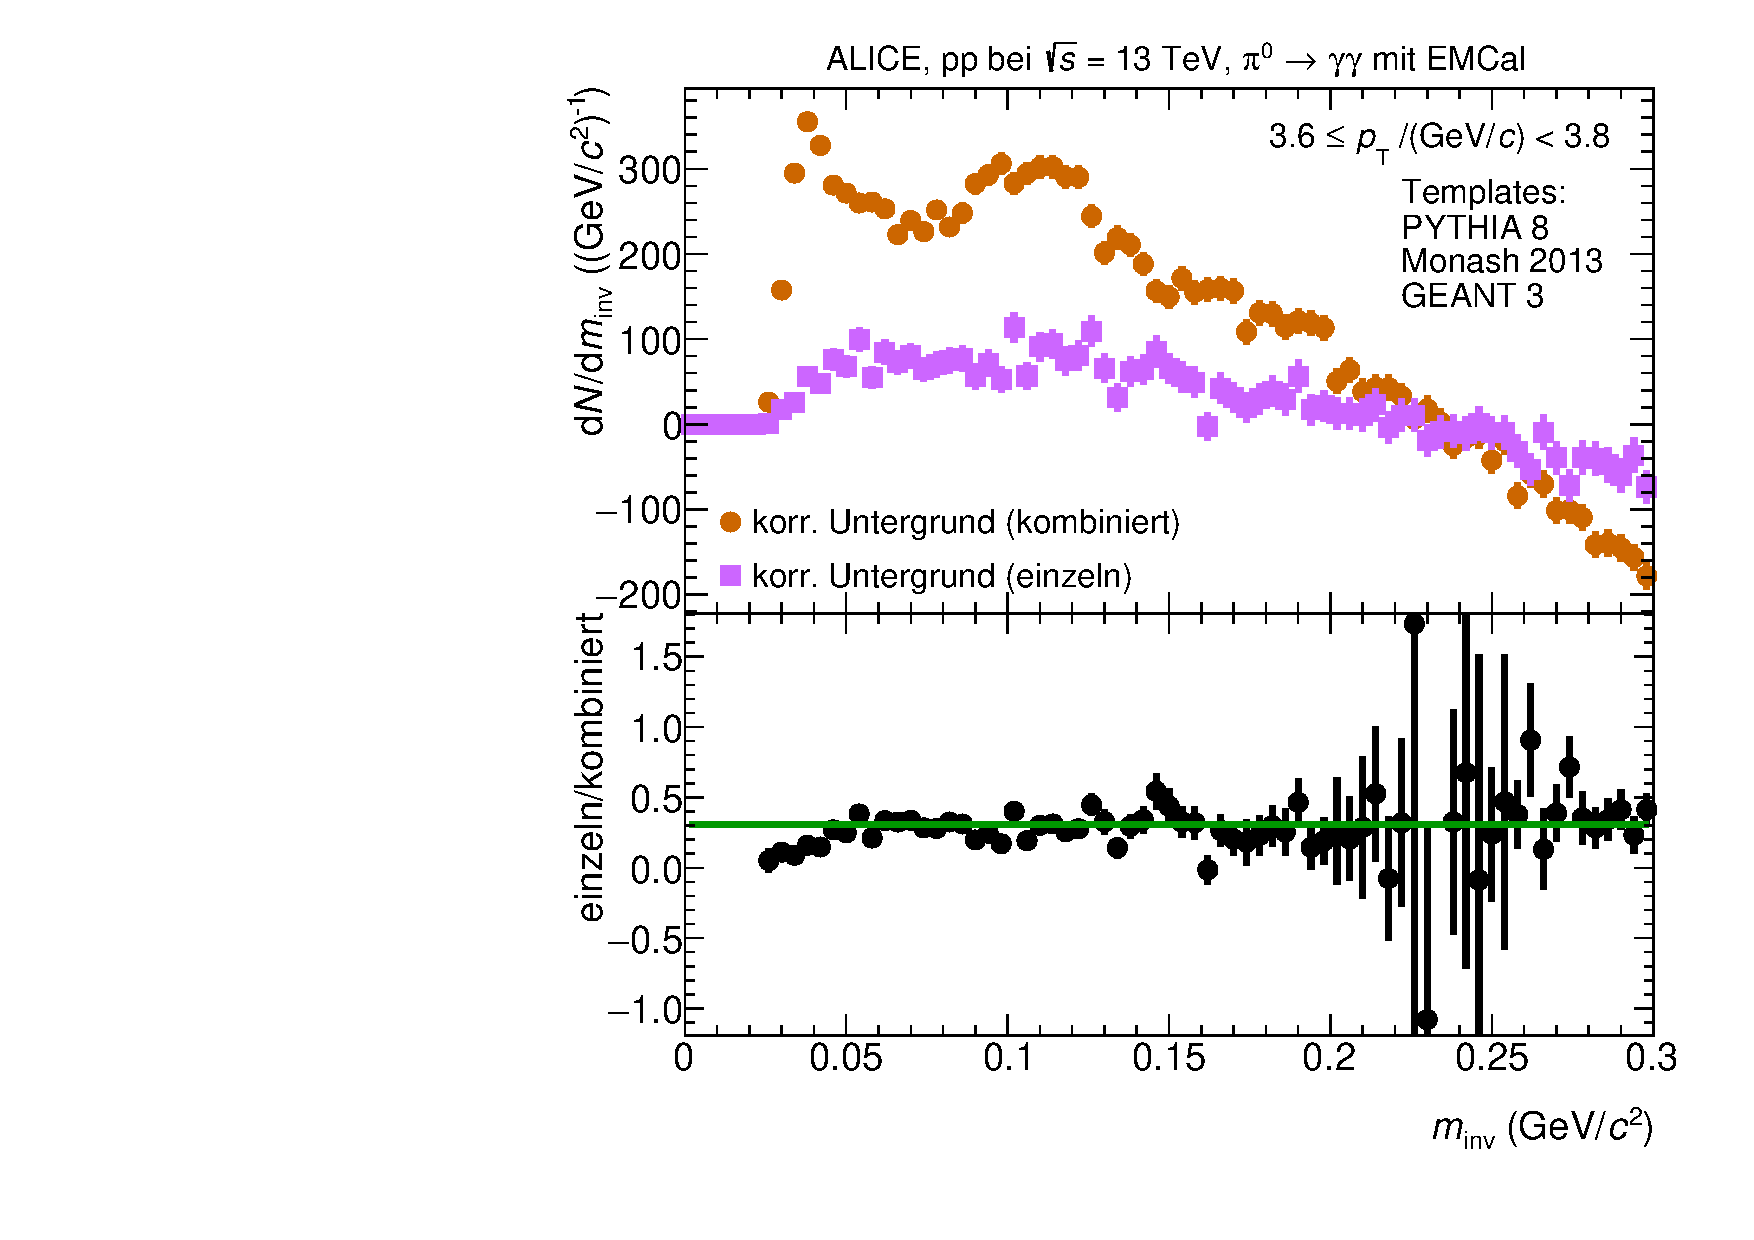
\includegraphics[width=.65\linewidth]{Anhang/BackgroundWithRatio12_Data_2016.pdf}\par
    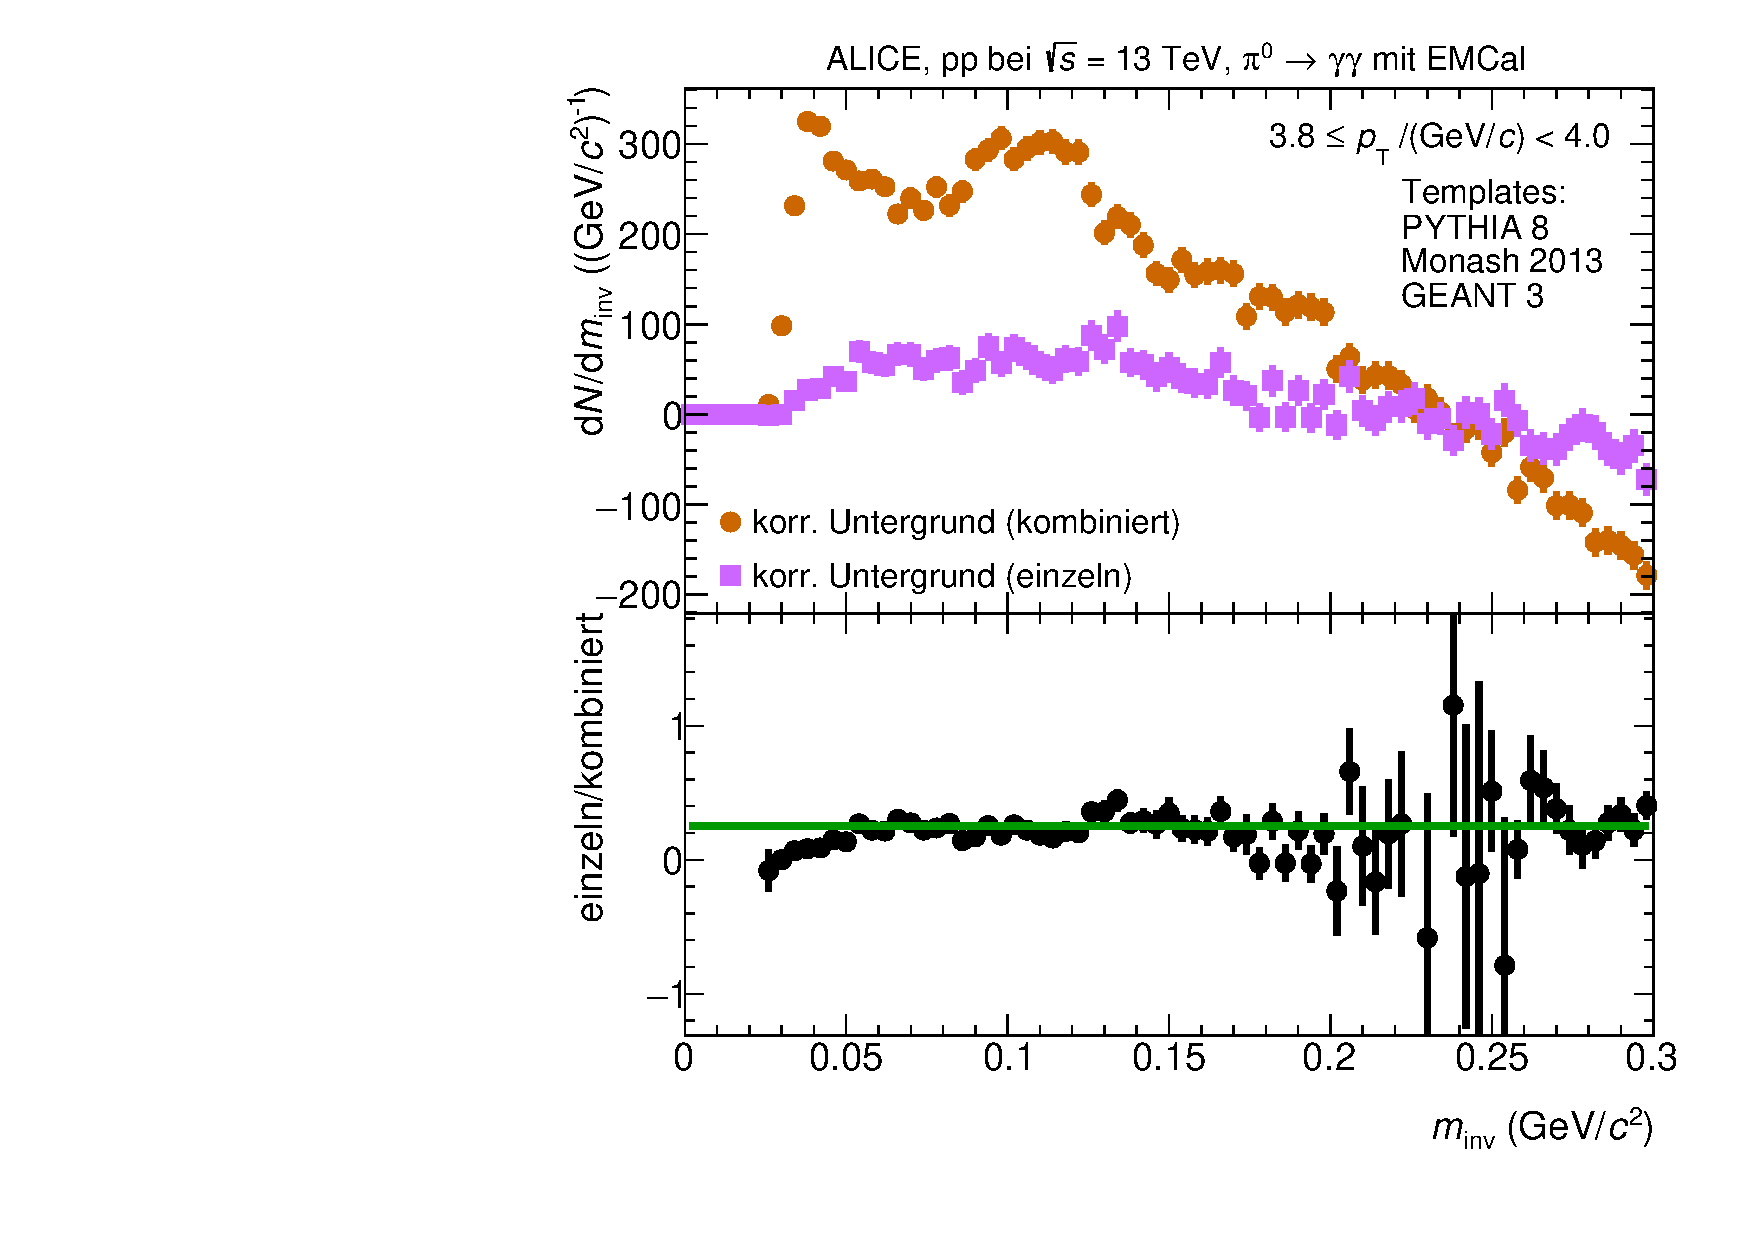
\includegraphics[width=.65\linewidth]{Anhang/BackgroundWithRatio13_Data_2016.pdf}\par
\end{multicols}
\begin{multicols}{2}
    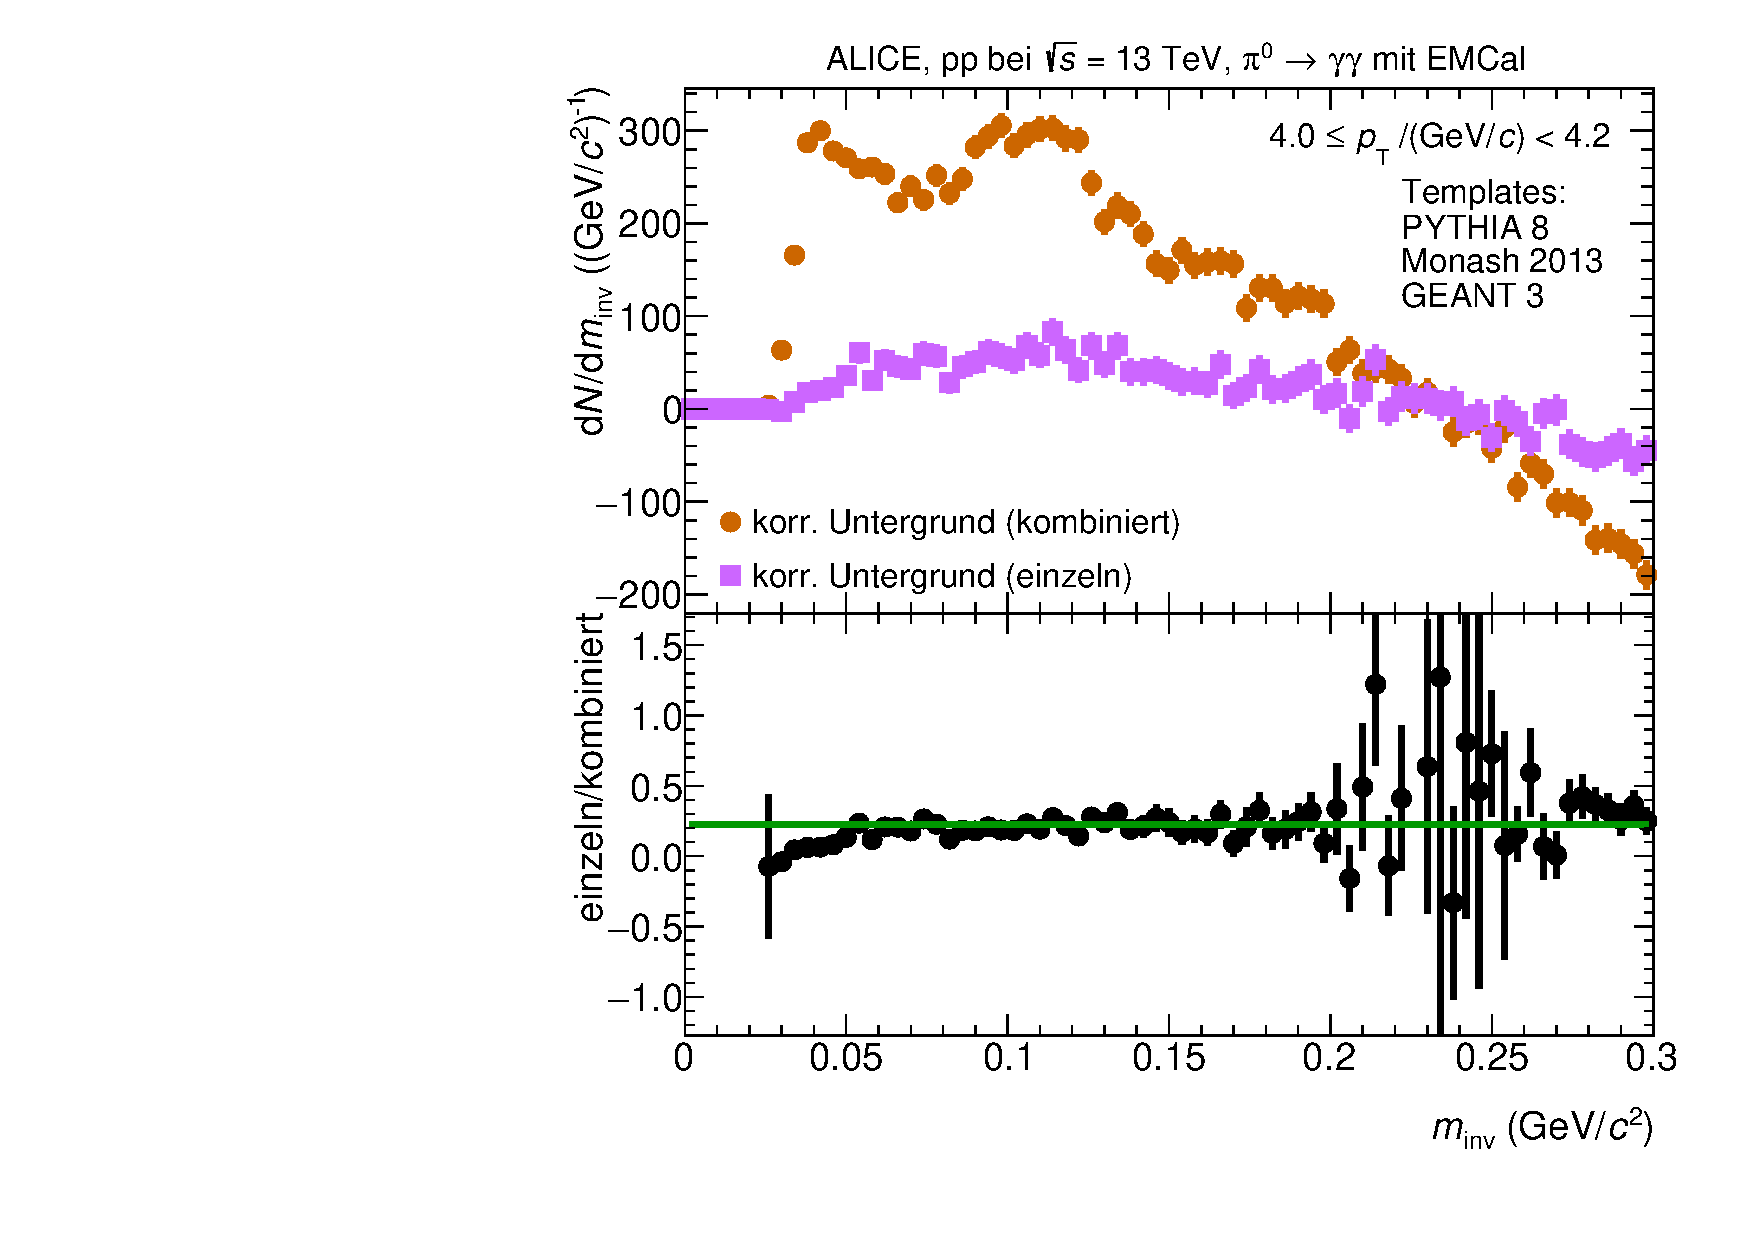
\includegraphics[width=.65\linewidth]{Anhang/BackgroundWithRatio14_Data_2016.pdf}\par
    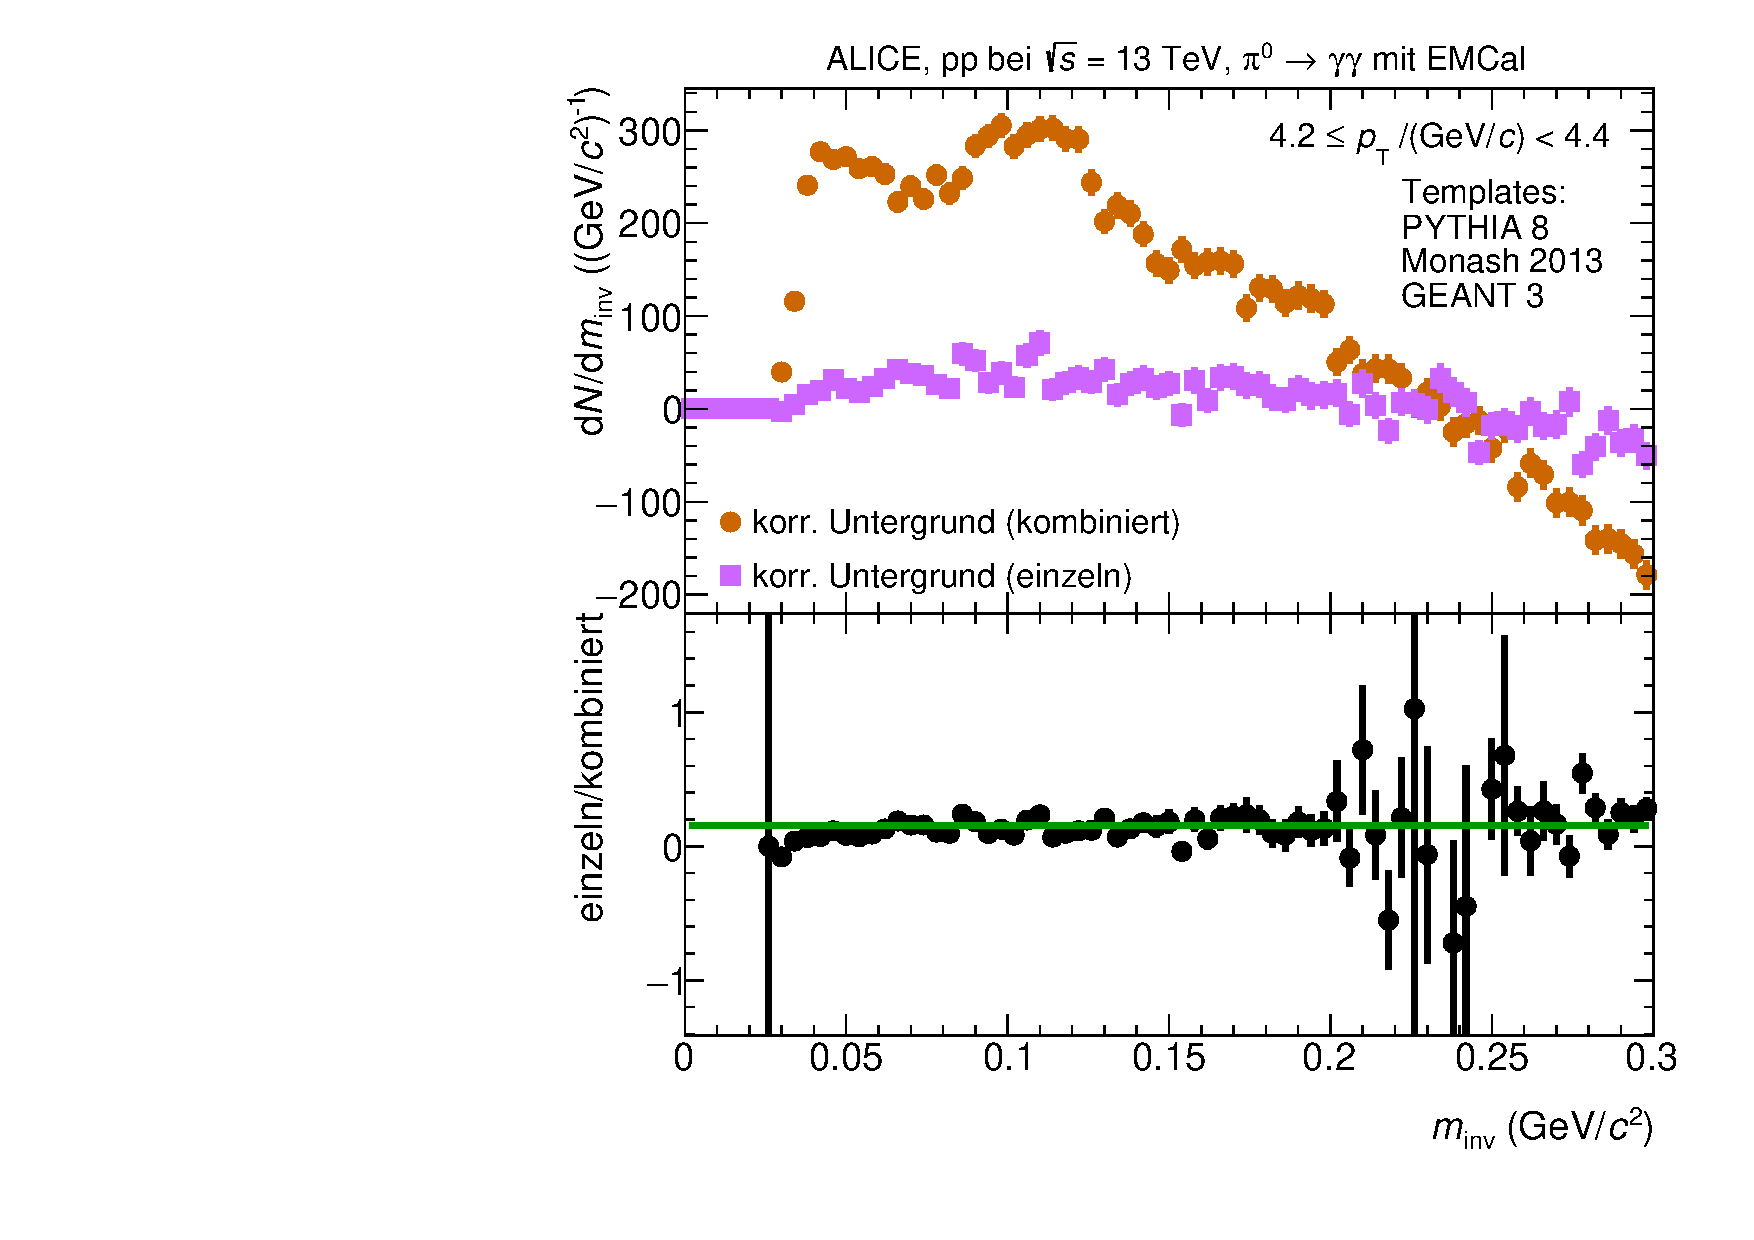
\includegraphics[width=.65\linewidth]{Anhang/BackgroundWithRatio15_Data_2016.pdf}\par
\end{multicols}
\end{figure*}
\clearpage

\begin{figure*}[t]
\centering
\begin{multicols}{2}
    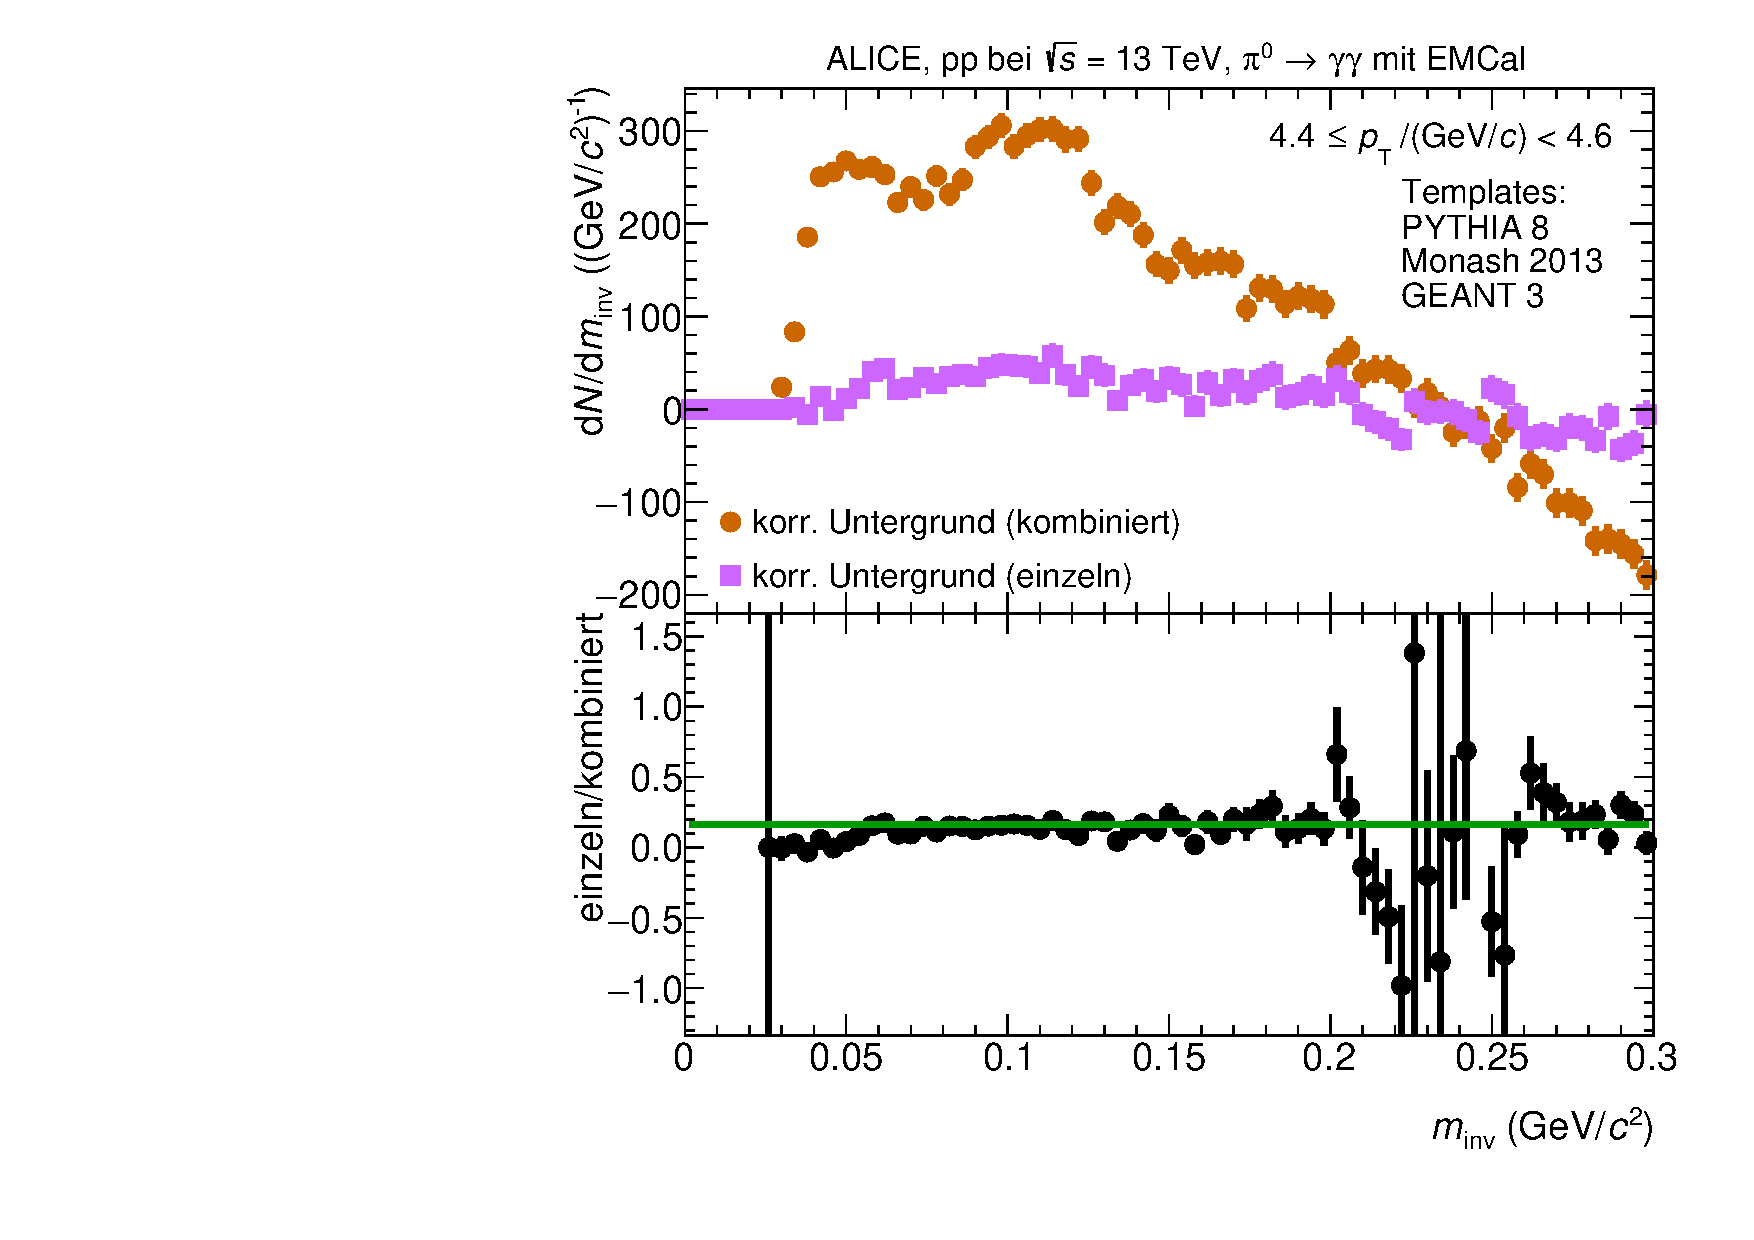
\includegraphics[width=.65\linewidth]{Anhang/BackgroundWithRatio16_Data_2016.pdf}\par 
    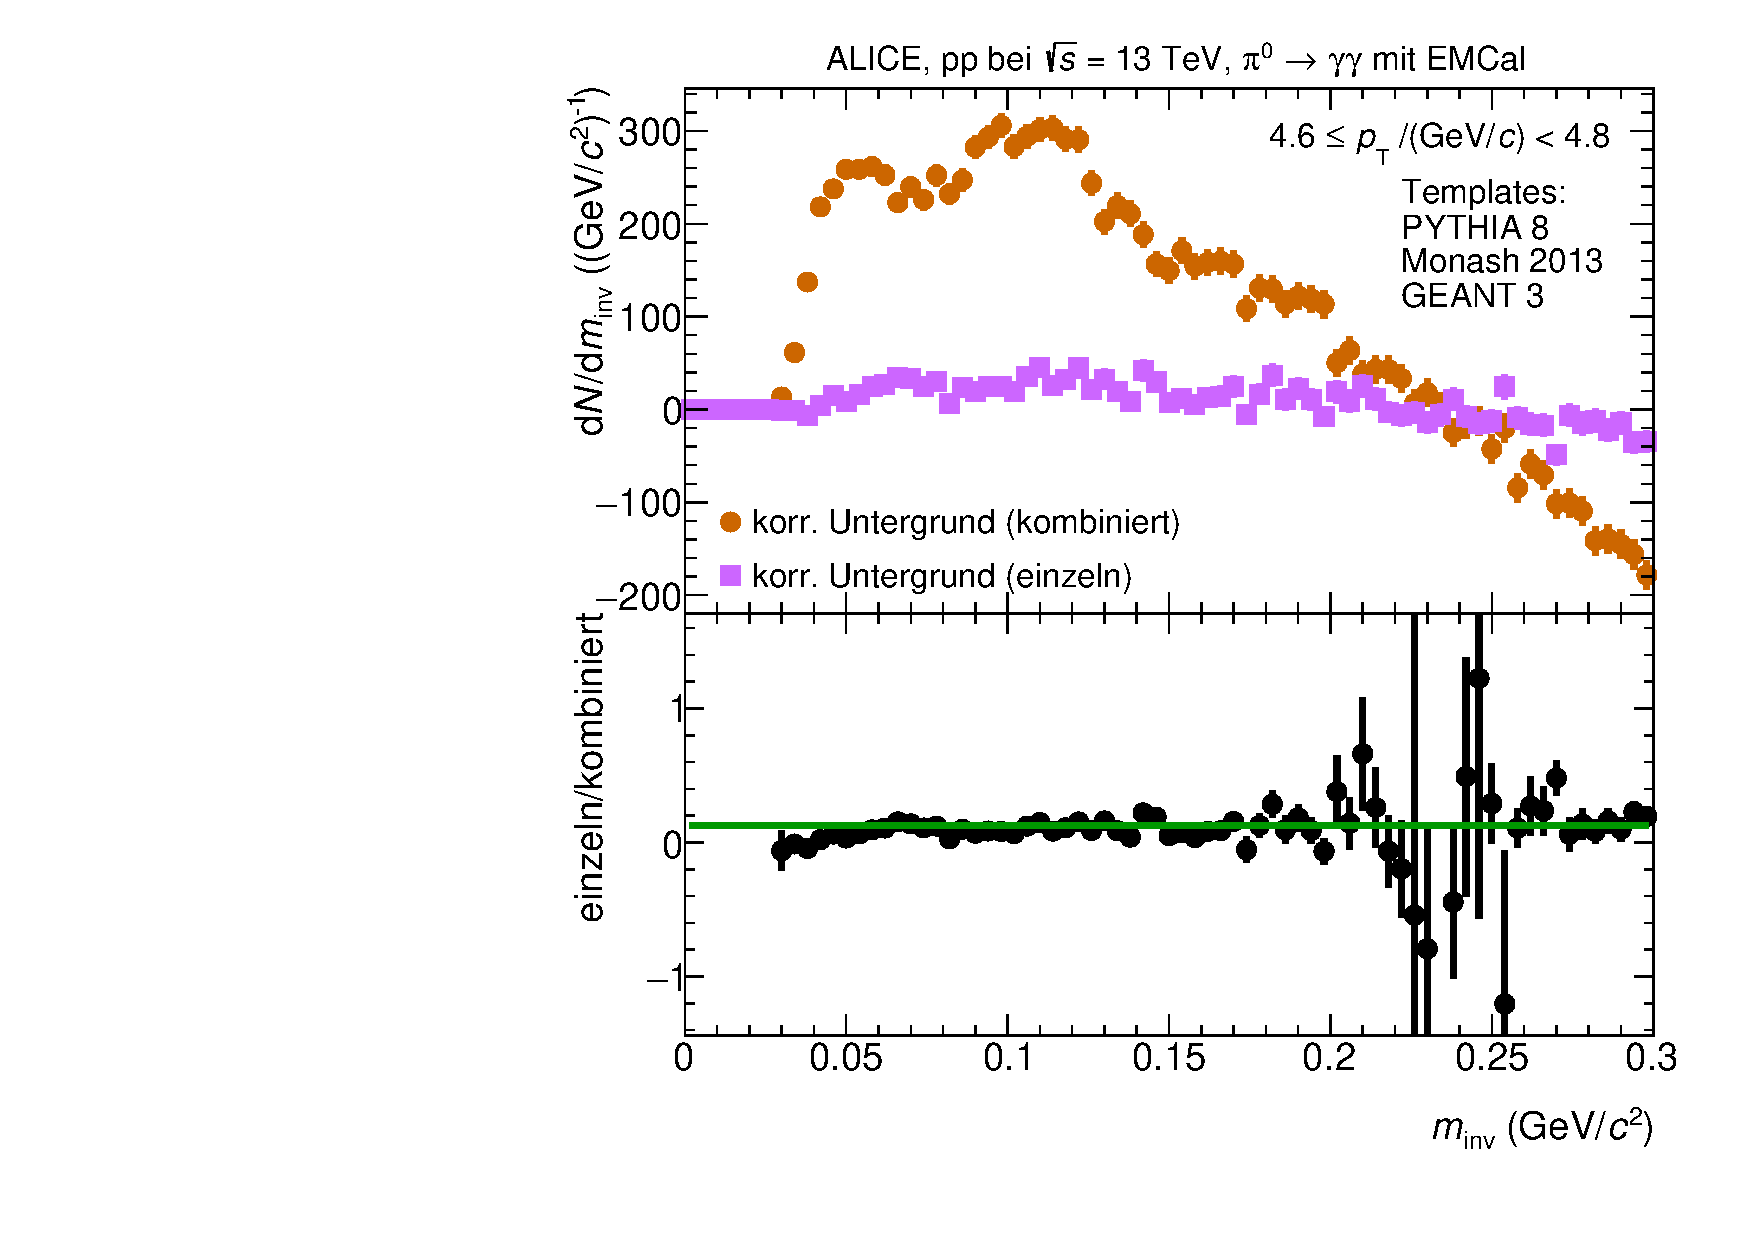
\includegraphics[width=.65\linewidth]{Anhang/BackgroundWithRatio17_Data_2016.pdf}\par 
\end{multicols}
\begin{multicols}{2}
    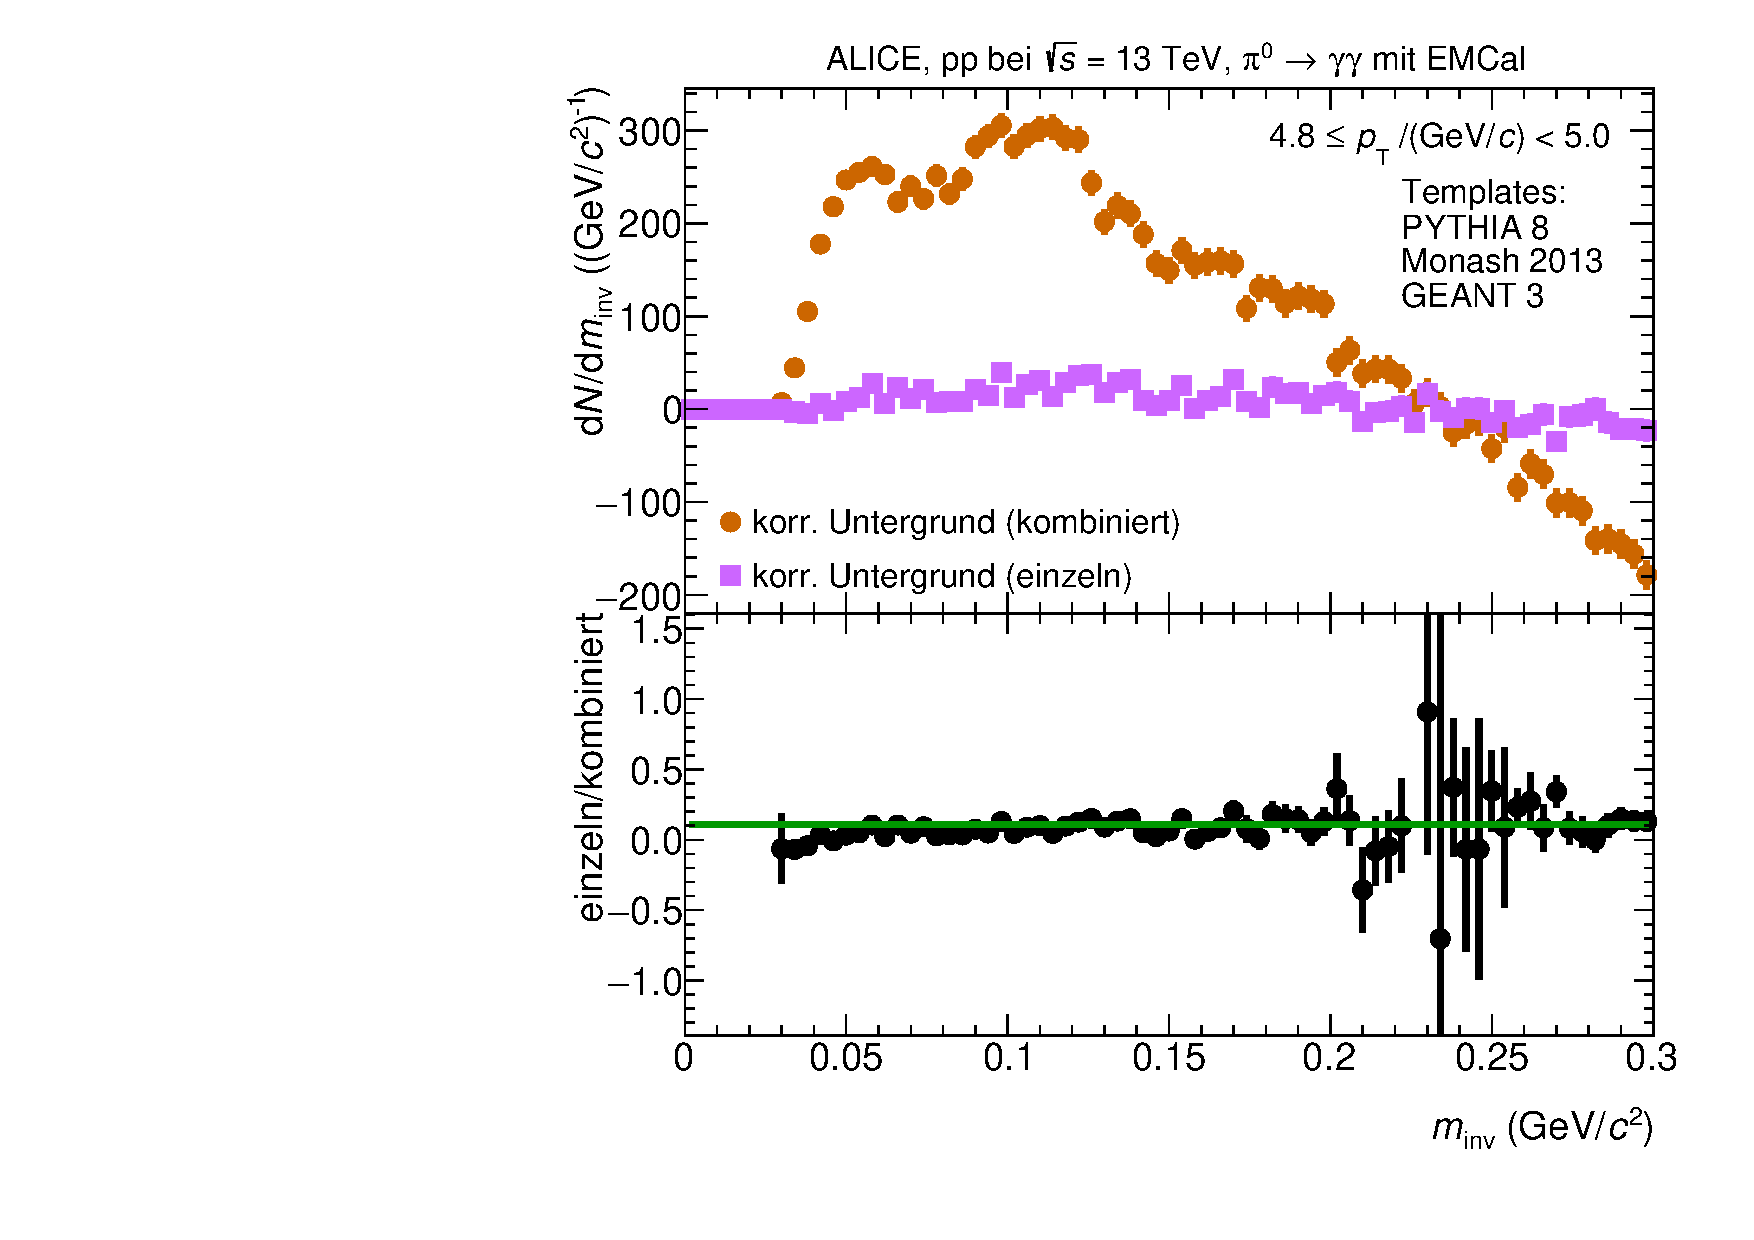
\includegraphics[width=.65\linewidth]{Anhang/BackgroundWithRatio18_Data_2016.pdf}\par
    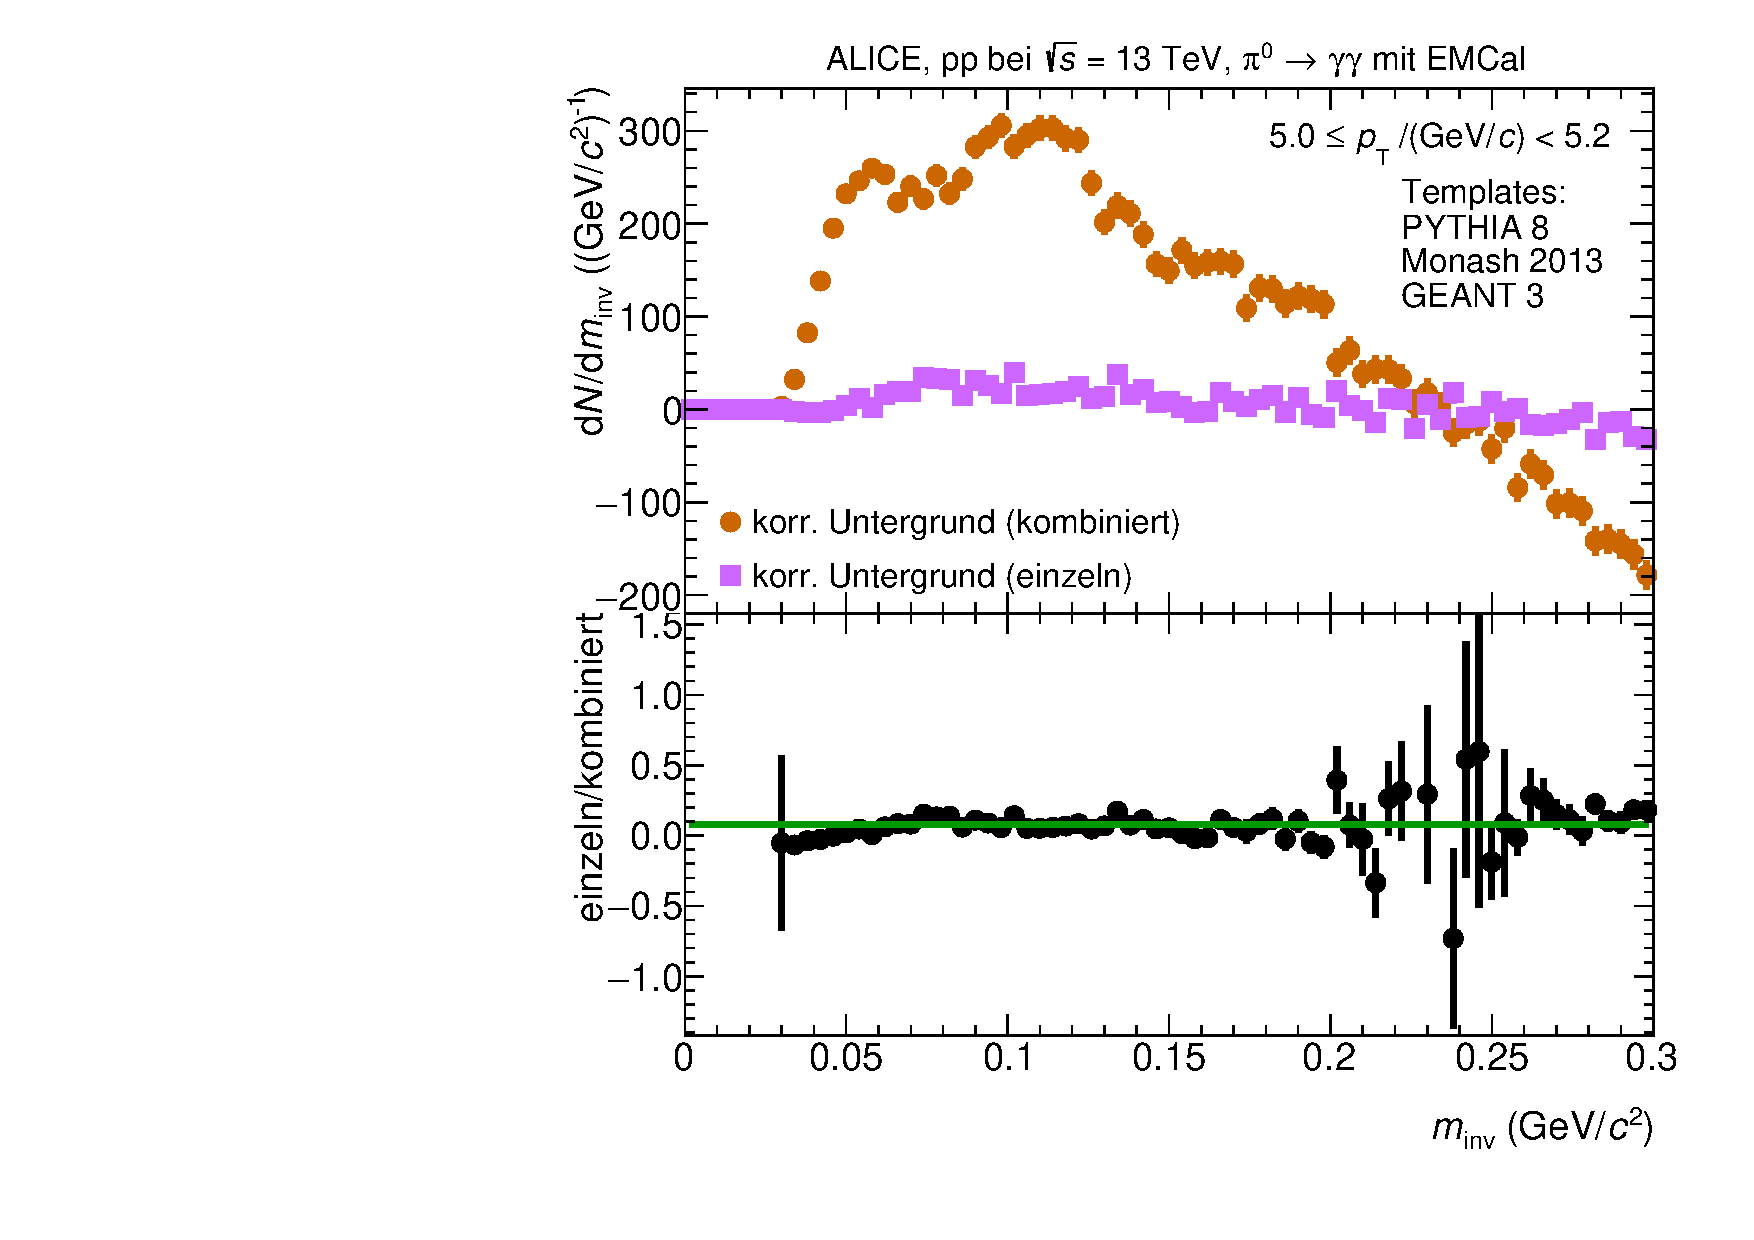
\includegraphics[width=.65\linewidth]{Anhang/BackgroundWithRatio19_Data_2016.pdf}\par
\end{multicols}
\begin{multicols}{2}
    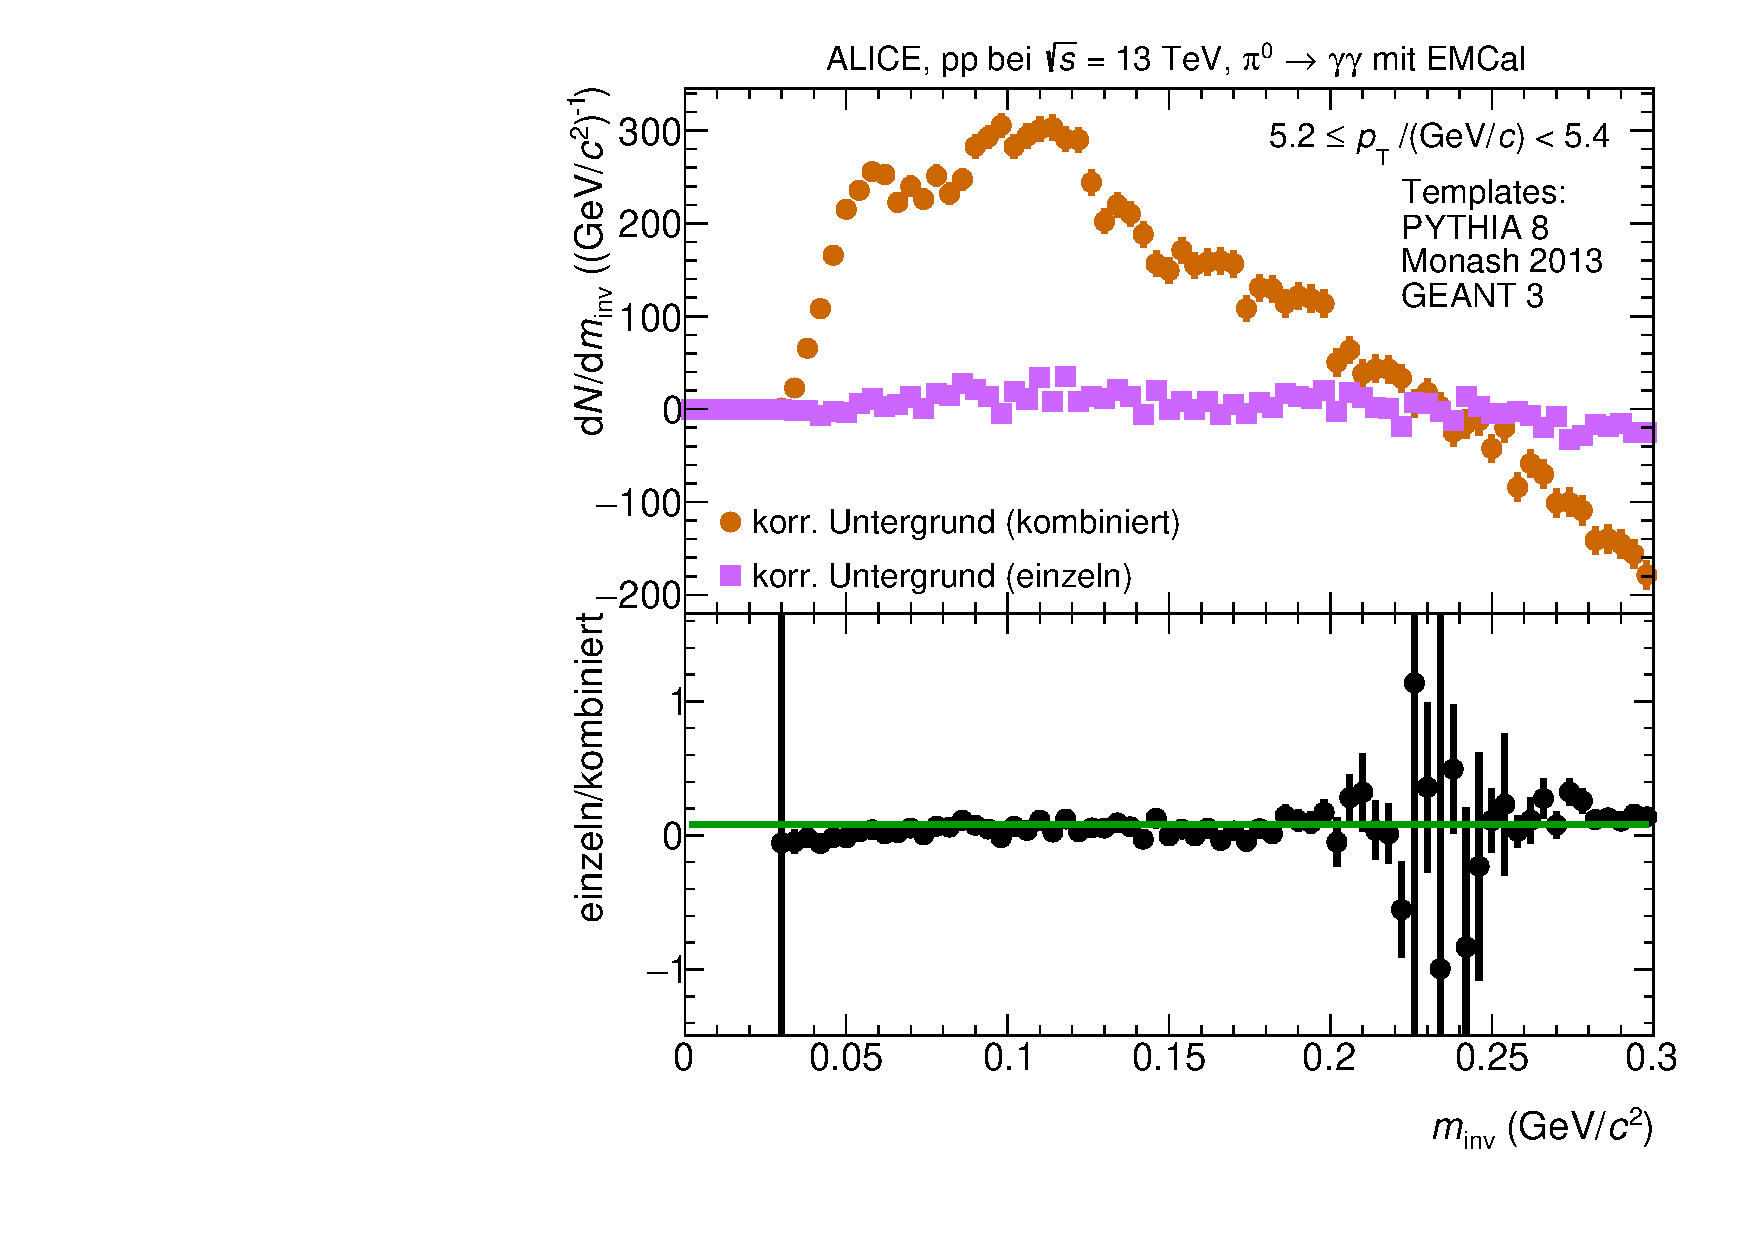
\includegraphics[width=.65\linewidth]{Anhang/BackgroundWithRatio20_Data_2016.pdf}\par
    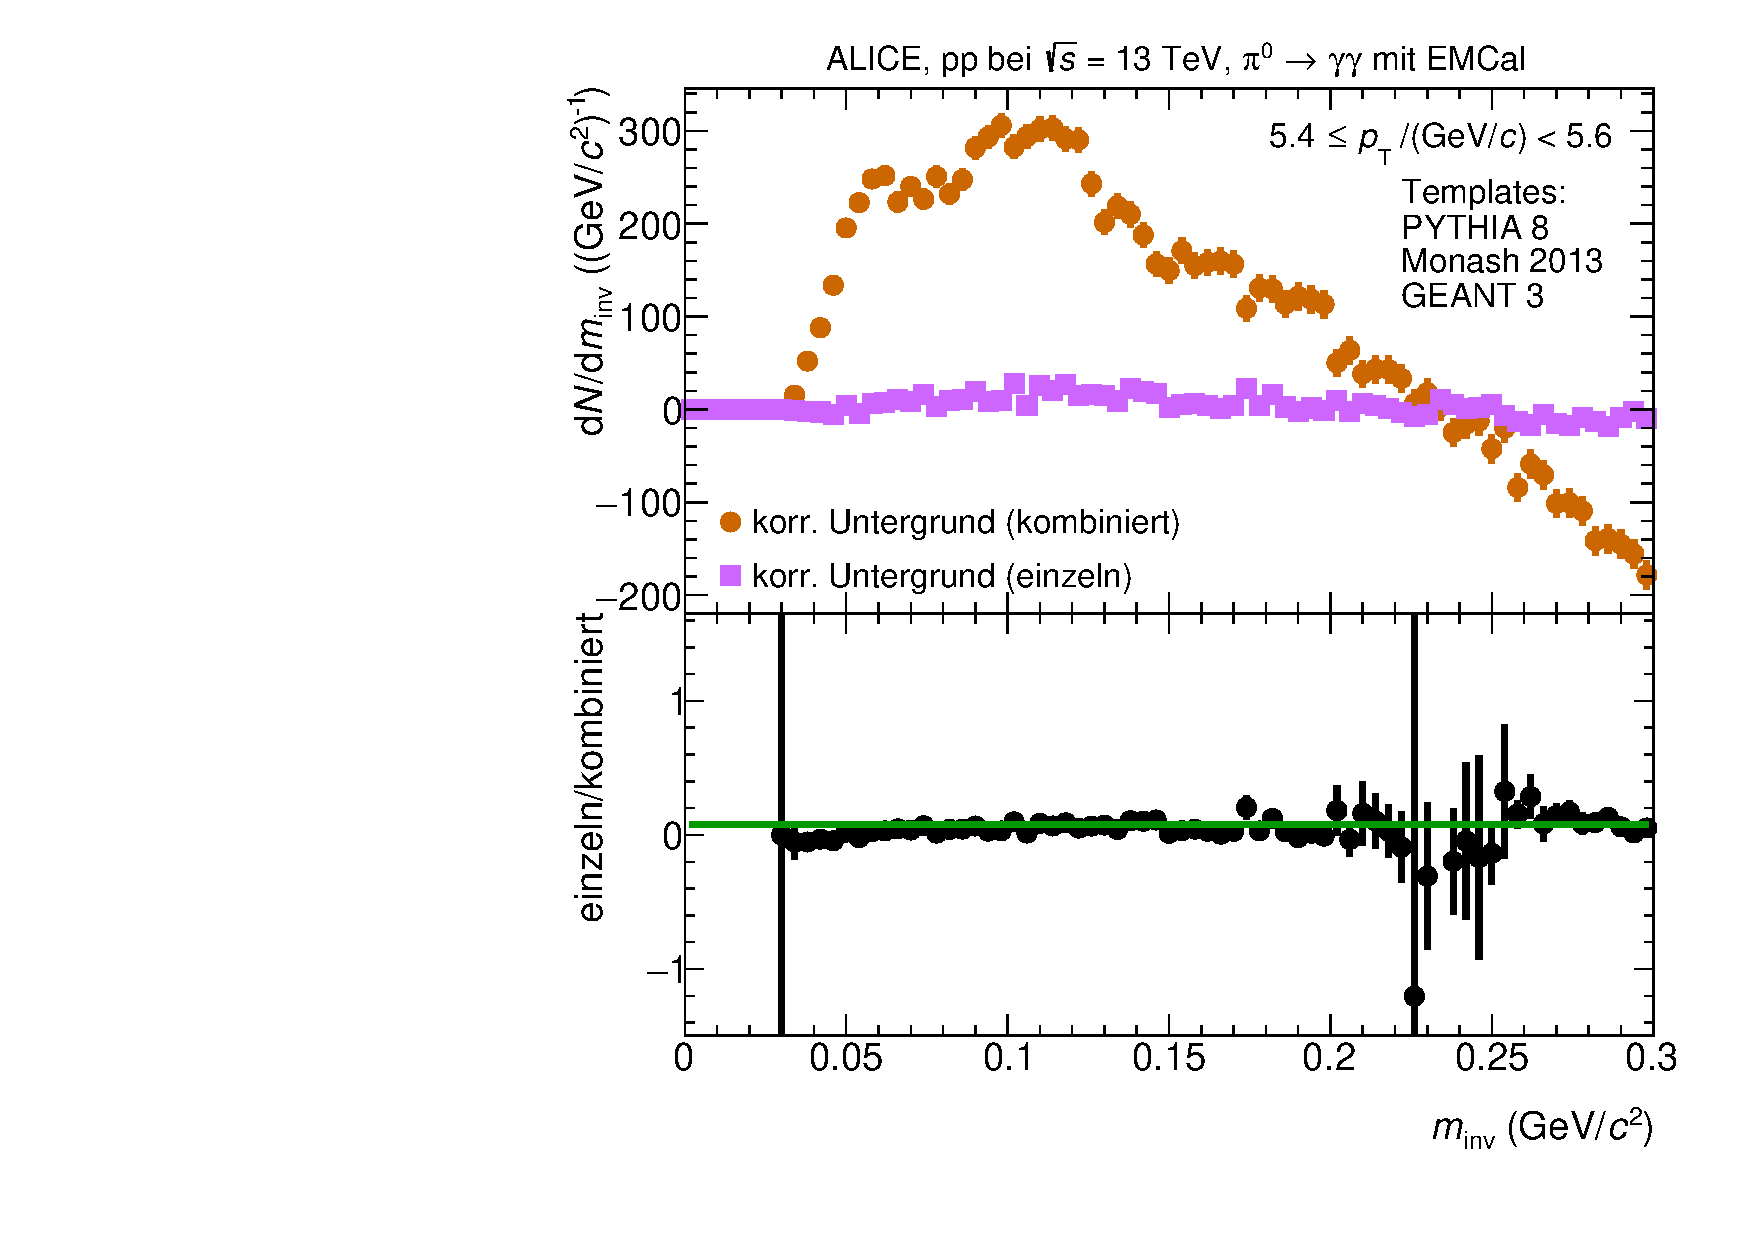
\includegraphics[width=.65\linewidth]{Anhang/BackgroundWithRatio21_Data_2016.pdf}\par
\end{multicols}
\begin{multicols}{2}
    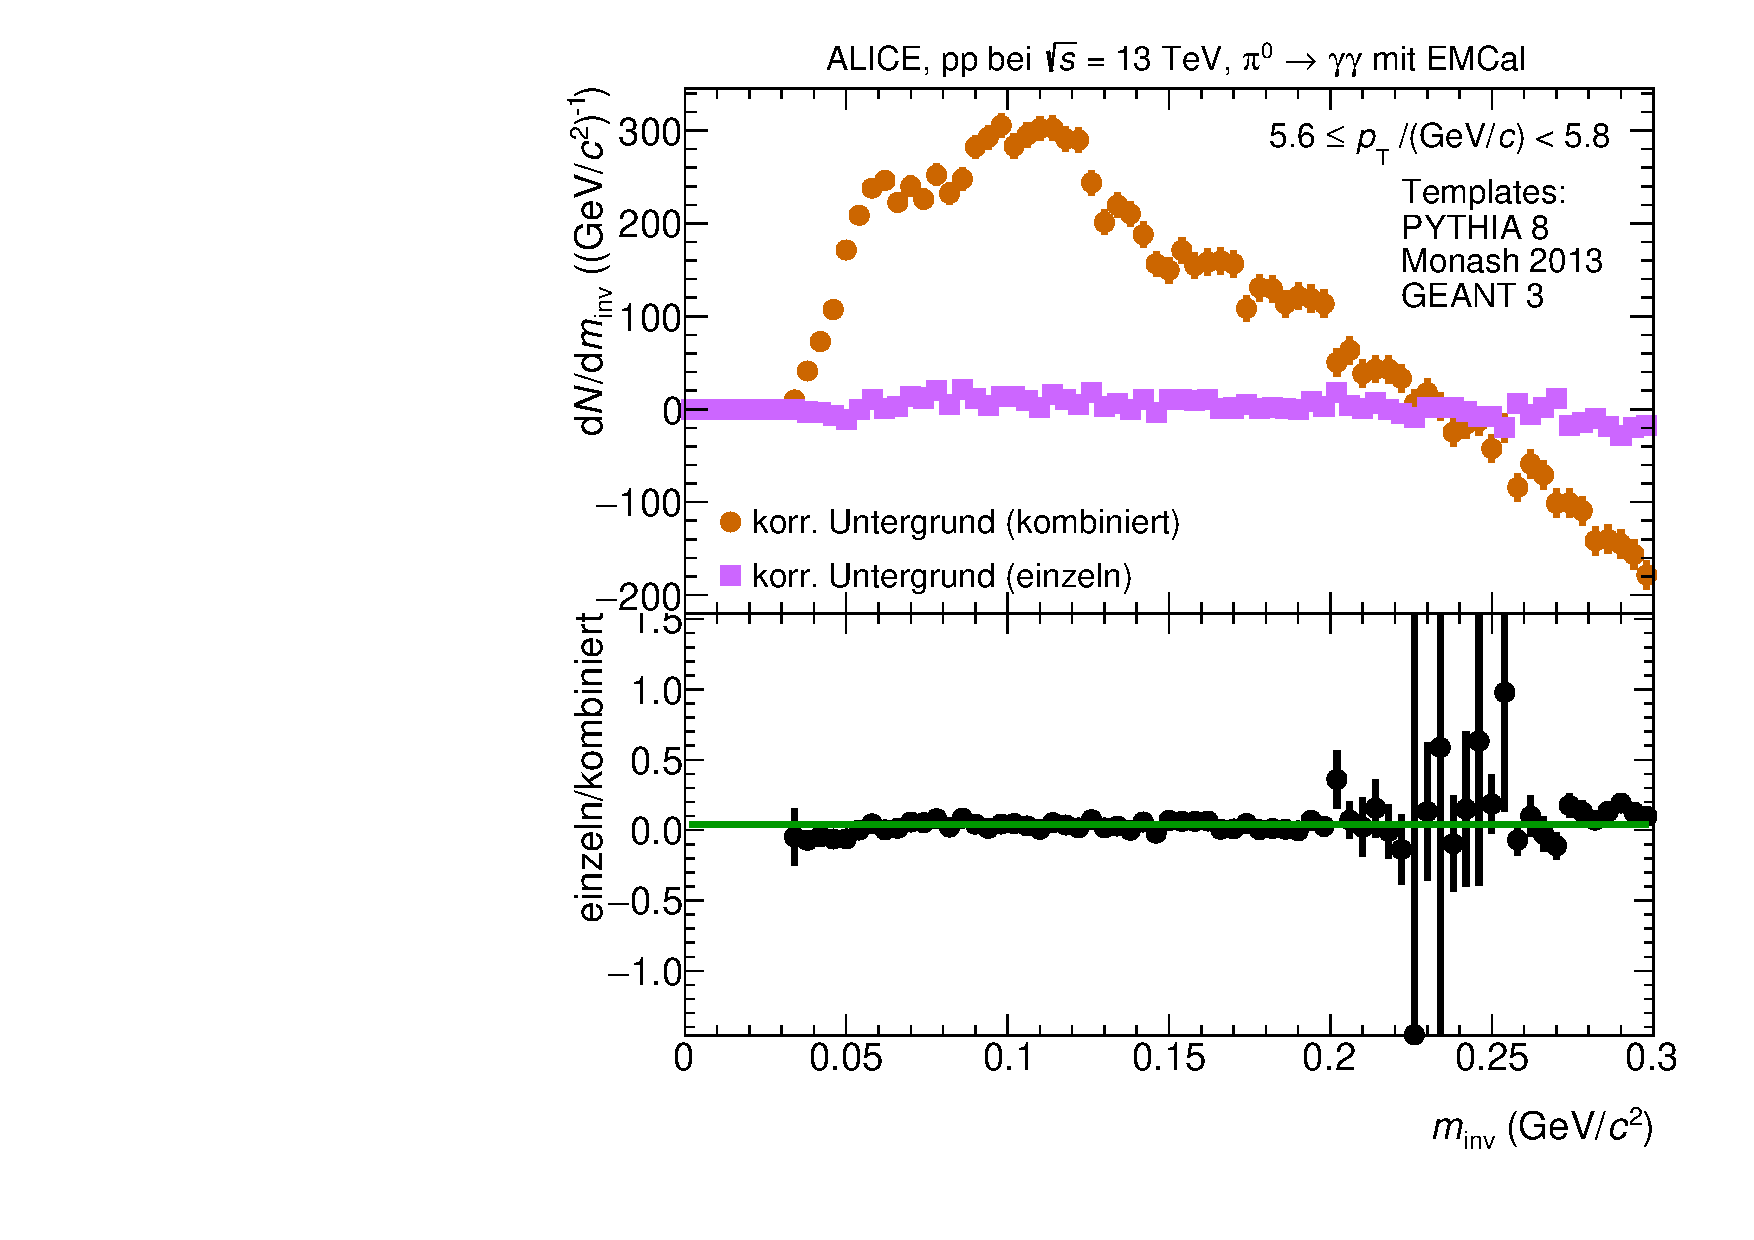
\includegraphics[width=.65\linewidth]{Anhang/BackgroundWithRatio22_Data_2016.pdf}\par
    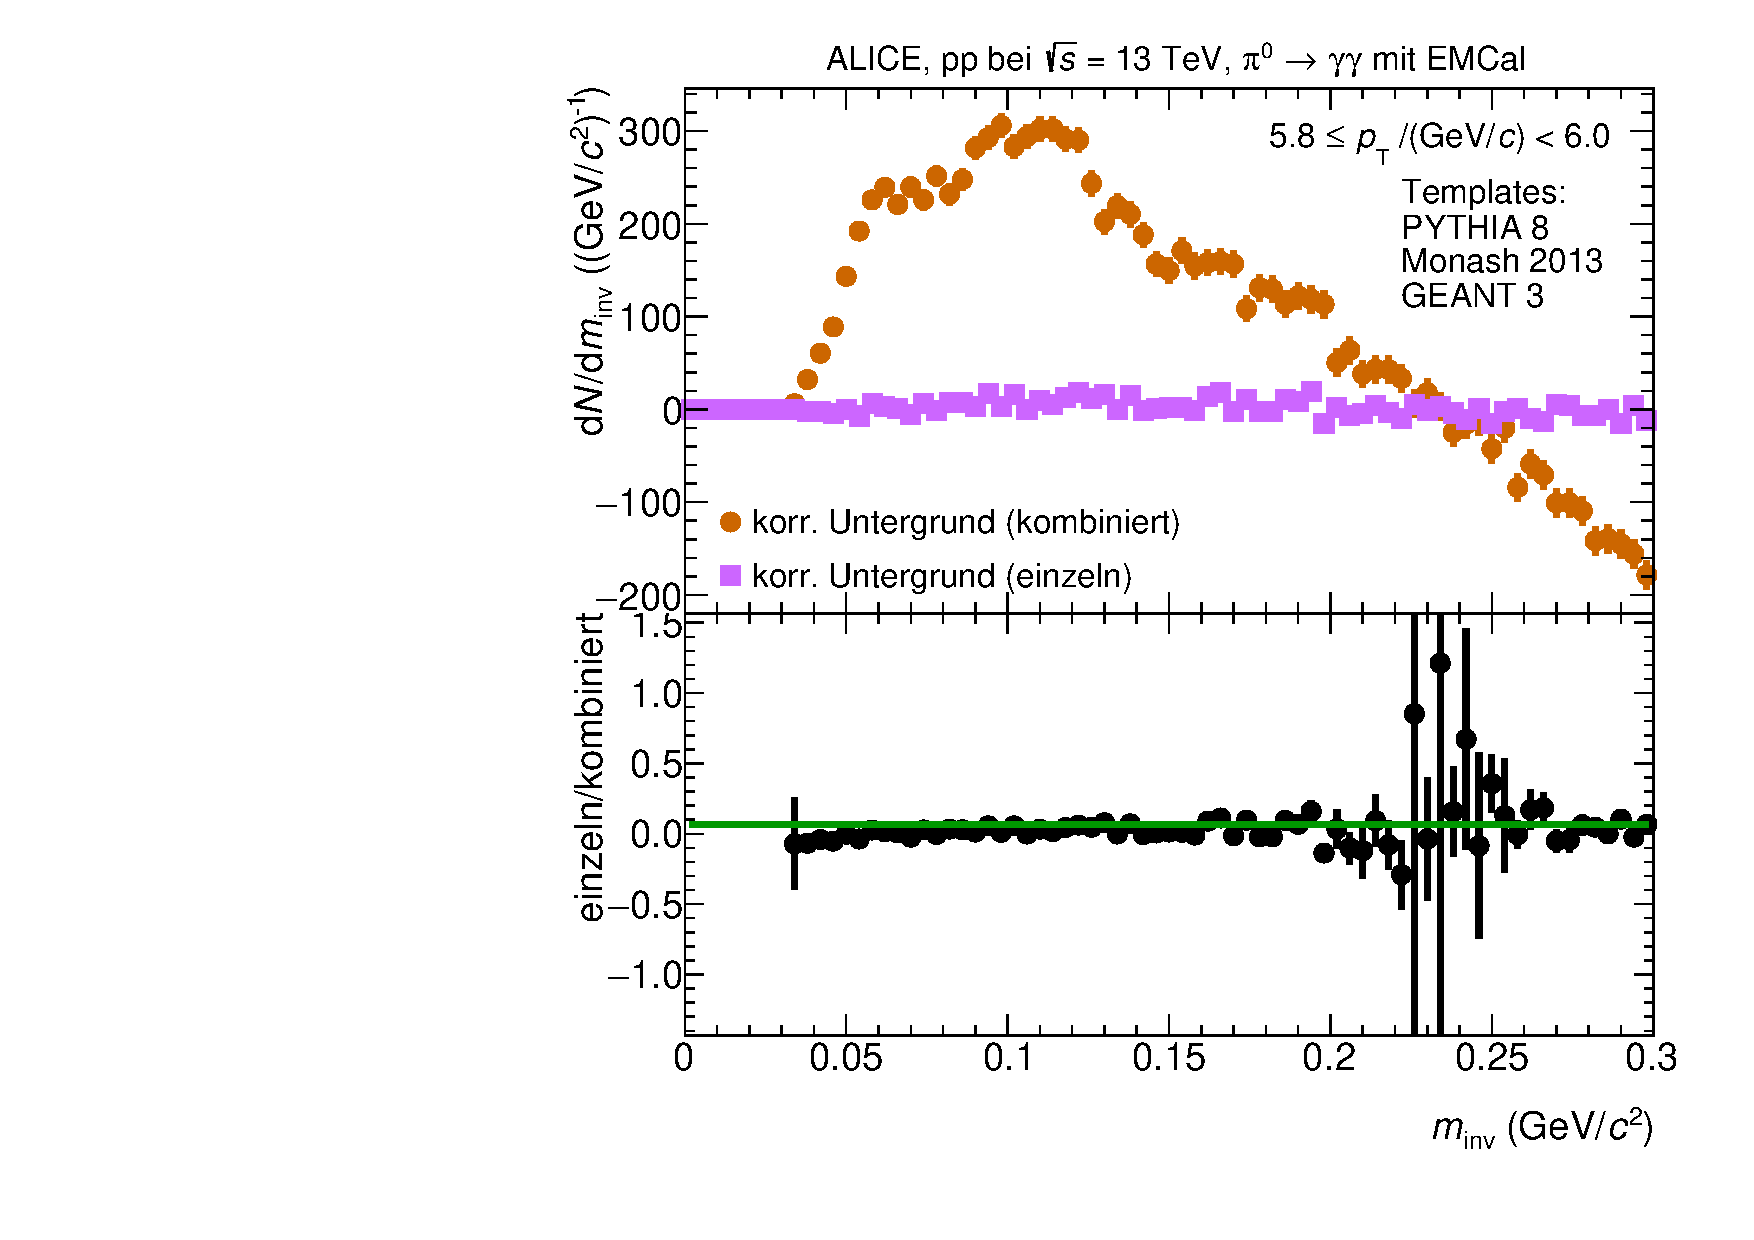
\includegraphics[width=.65\linewidth]{Anhang/BackgroundWithRatio23_Data_2016.pdf}\par
\end{multicols}
\end{figure*}
\clearpage

\begin{figure*}[t]
\centering
\begin{multicols}{2}
    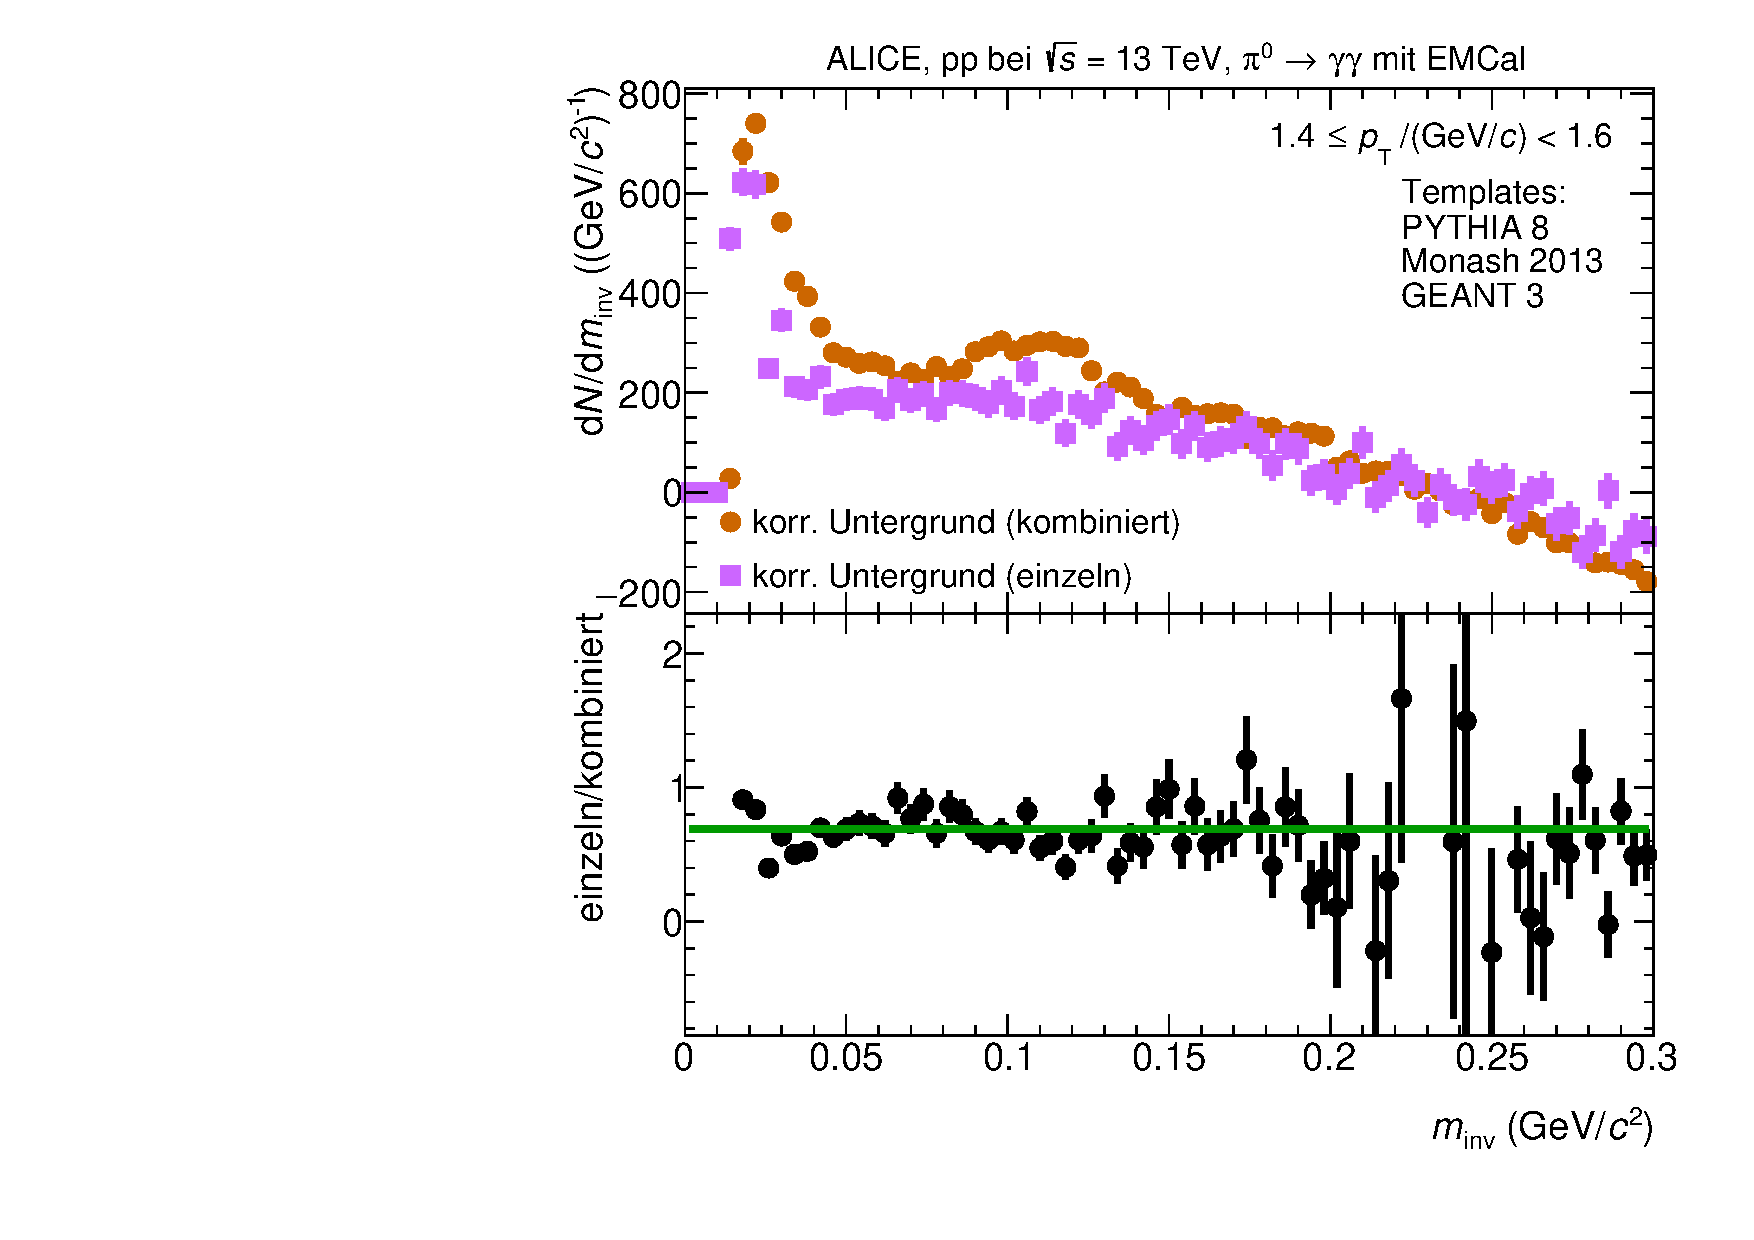
\includegraphics[width=.65\linewidth]{Anhang/BackgroundWithRatio01_Data_2016.pdf}\par 
    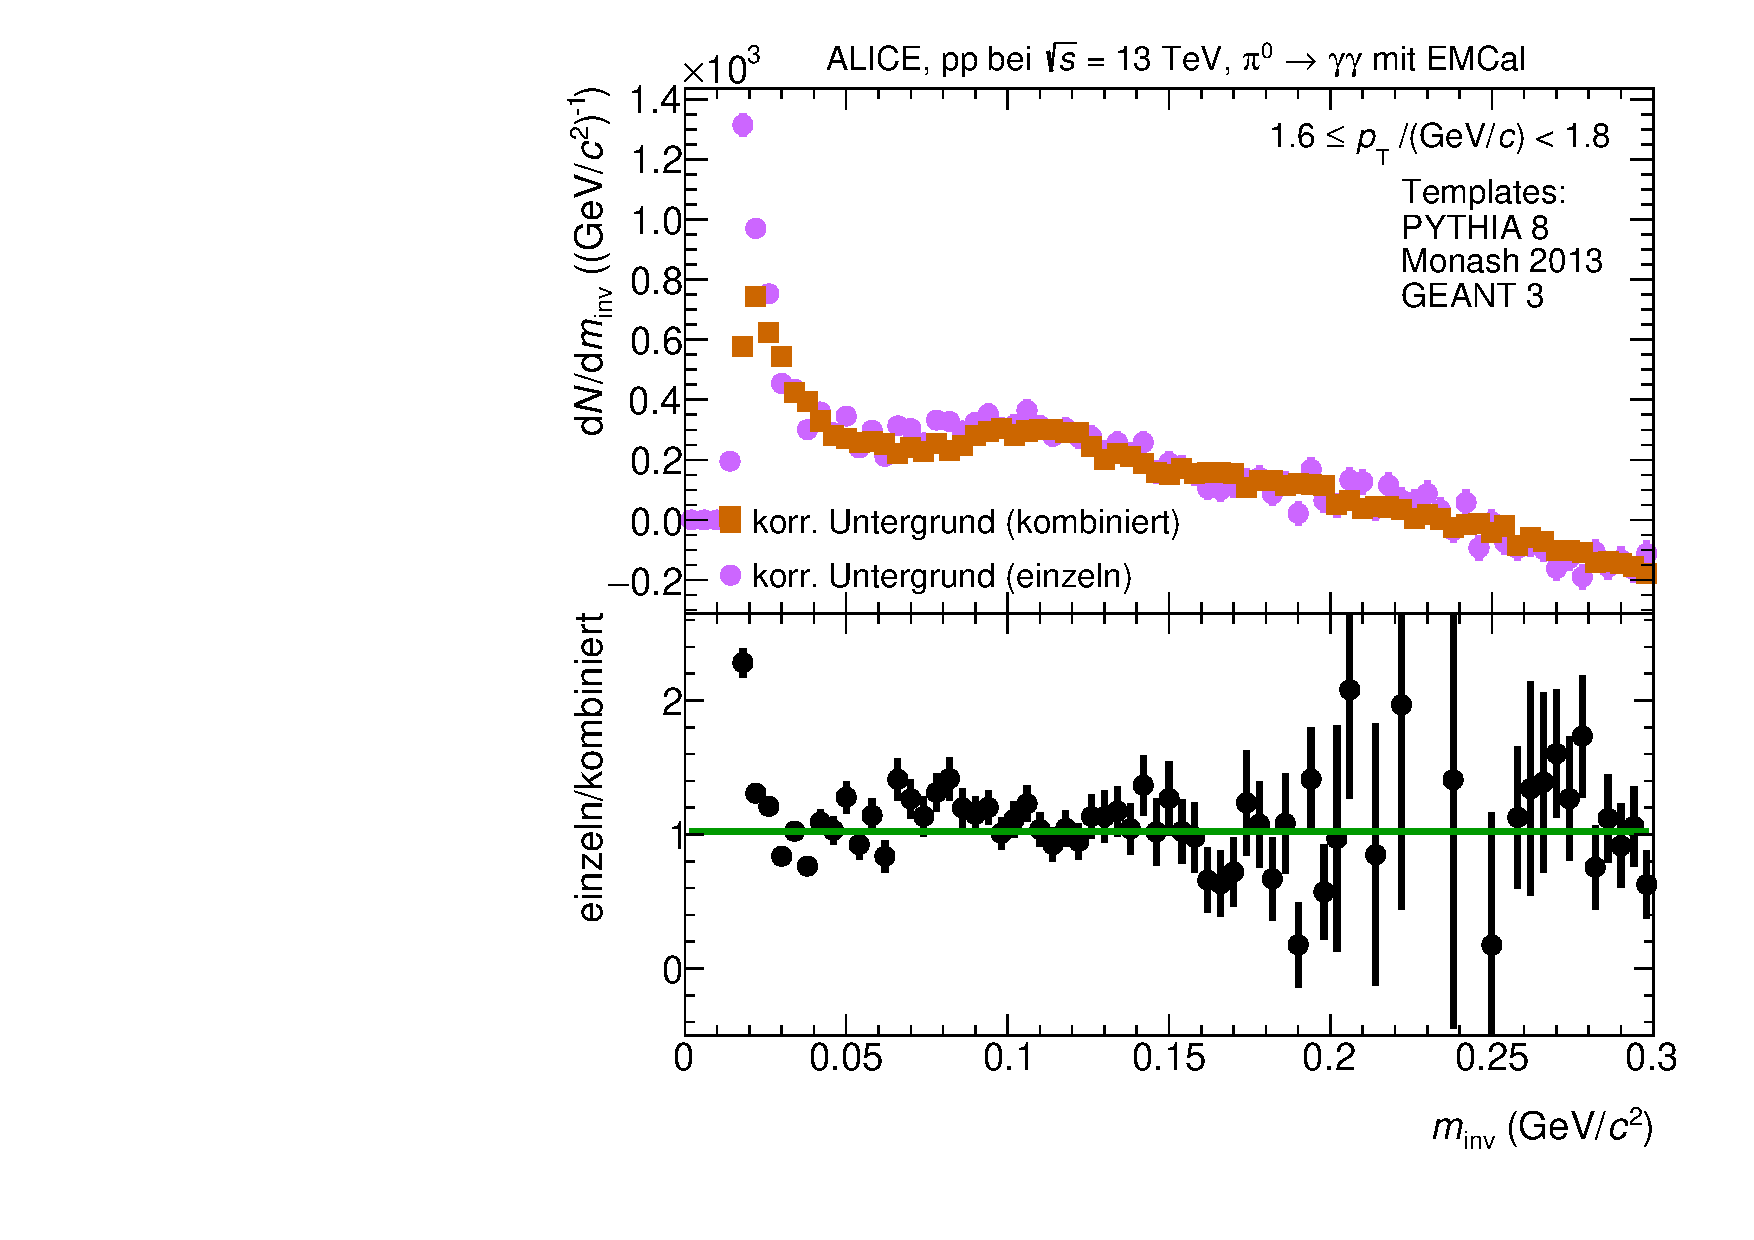
\includegraphics[width=.65\linewidth]{Anhang/BackgroundWithRatio02_Data_2016.pdf}\par  %NEEDS TO BE CHANGED
\end{multicols}
\begin{multicols}{2}
    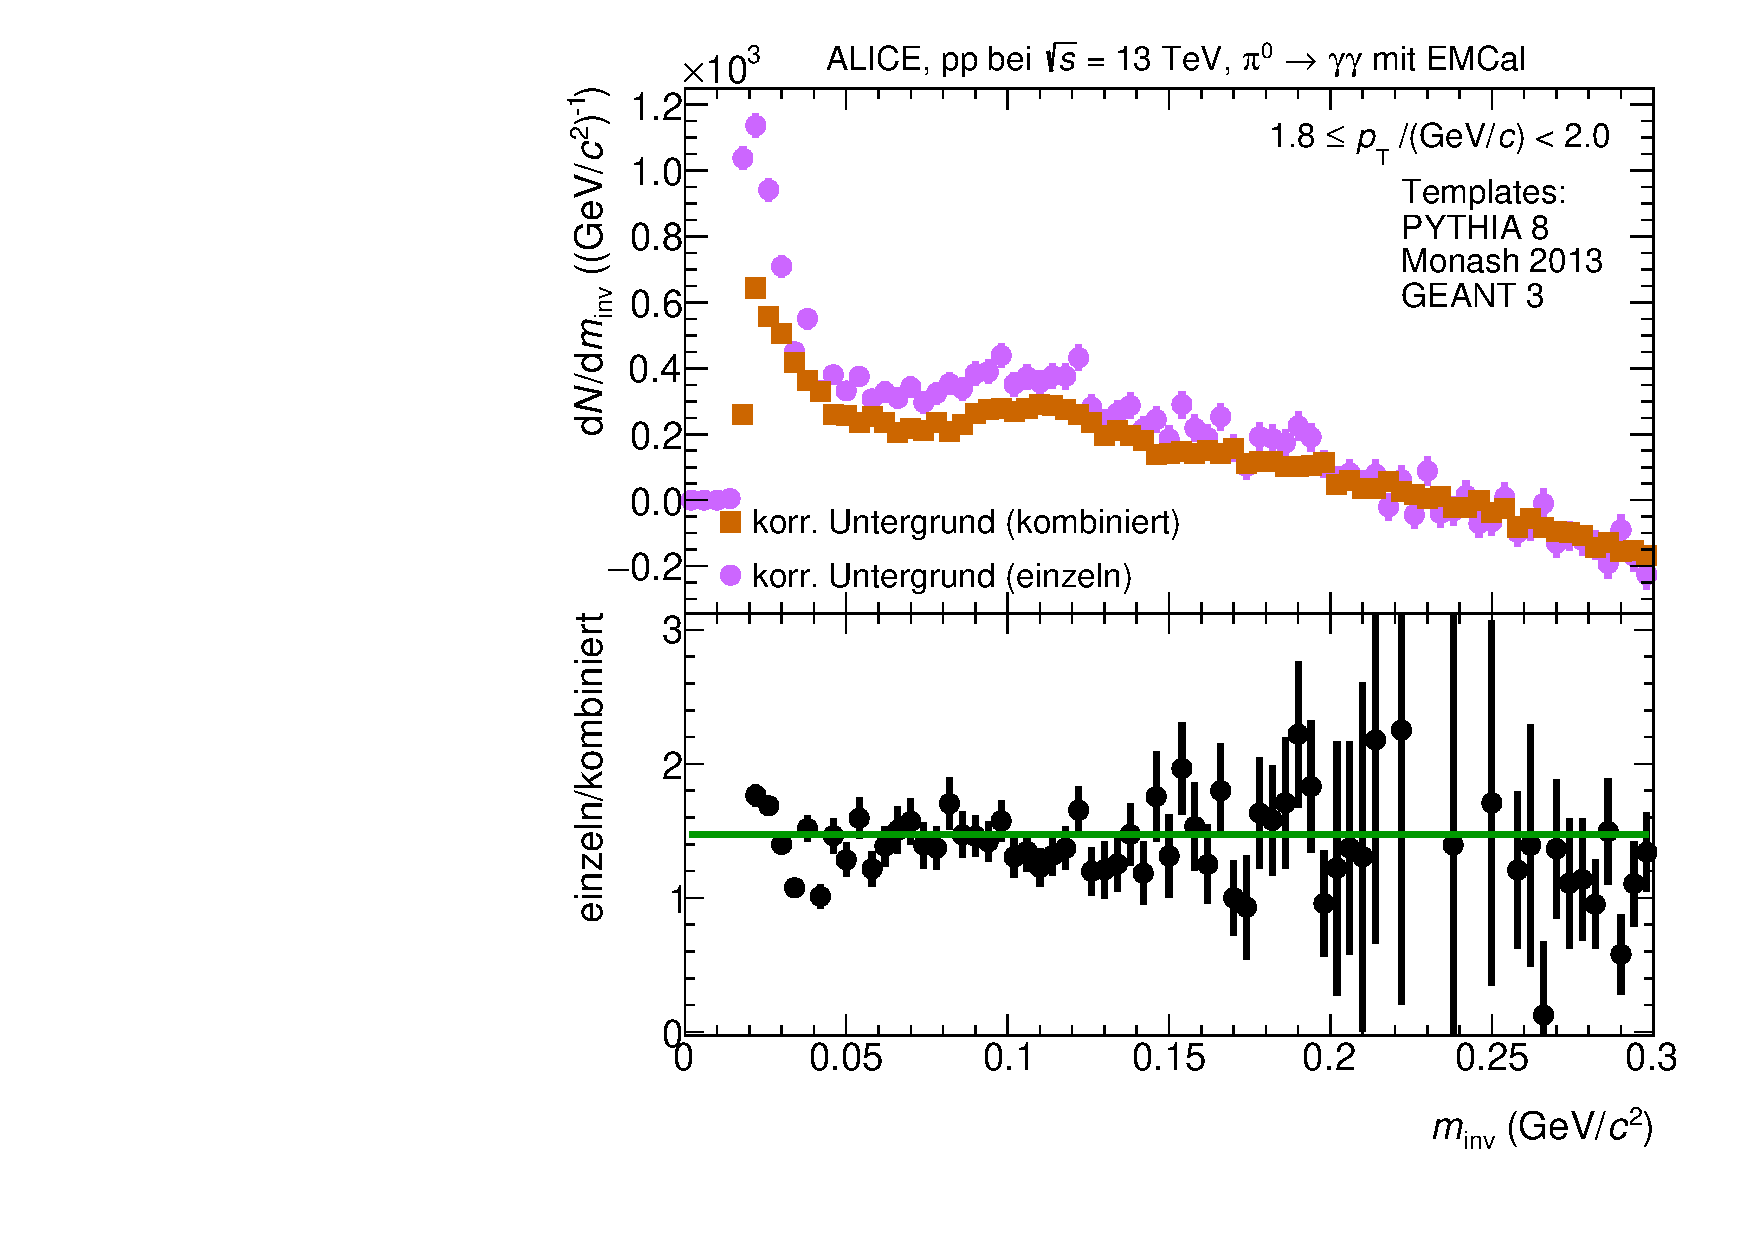
\includegraphics[width=.65\linewidth]{Anhang/BackgroundWithRatio03_Data_2016.pdf}\par
    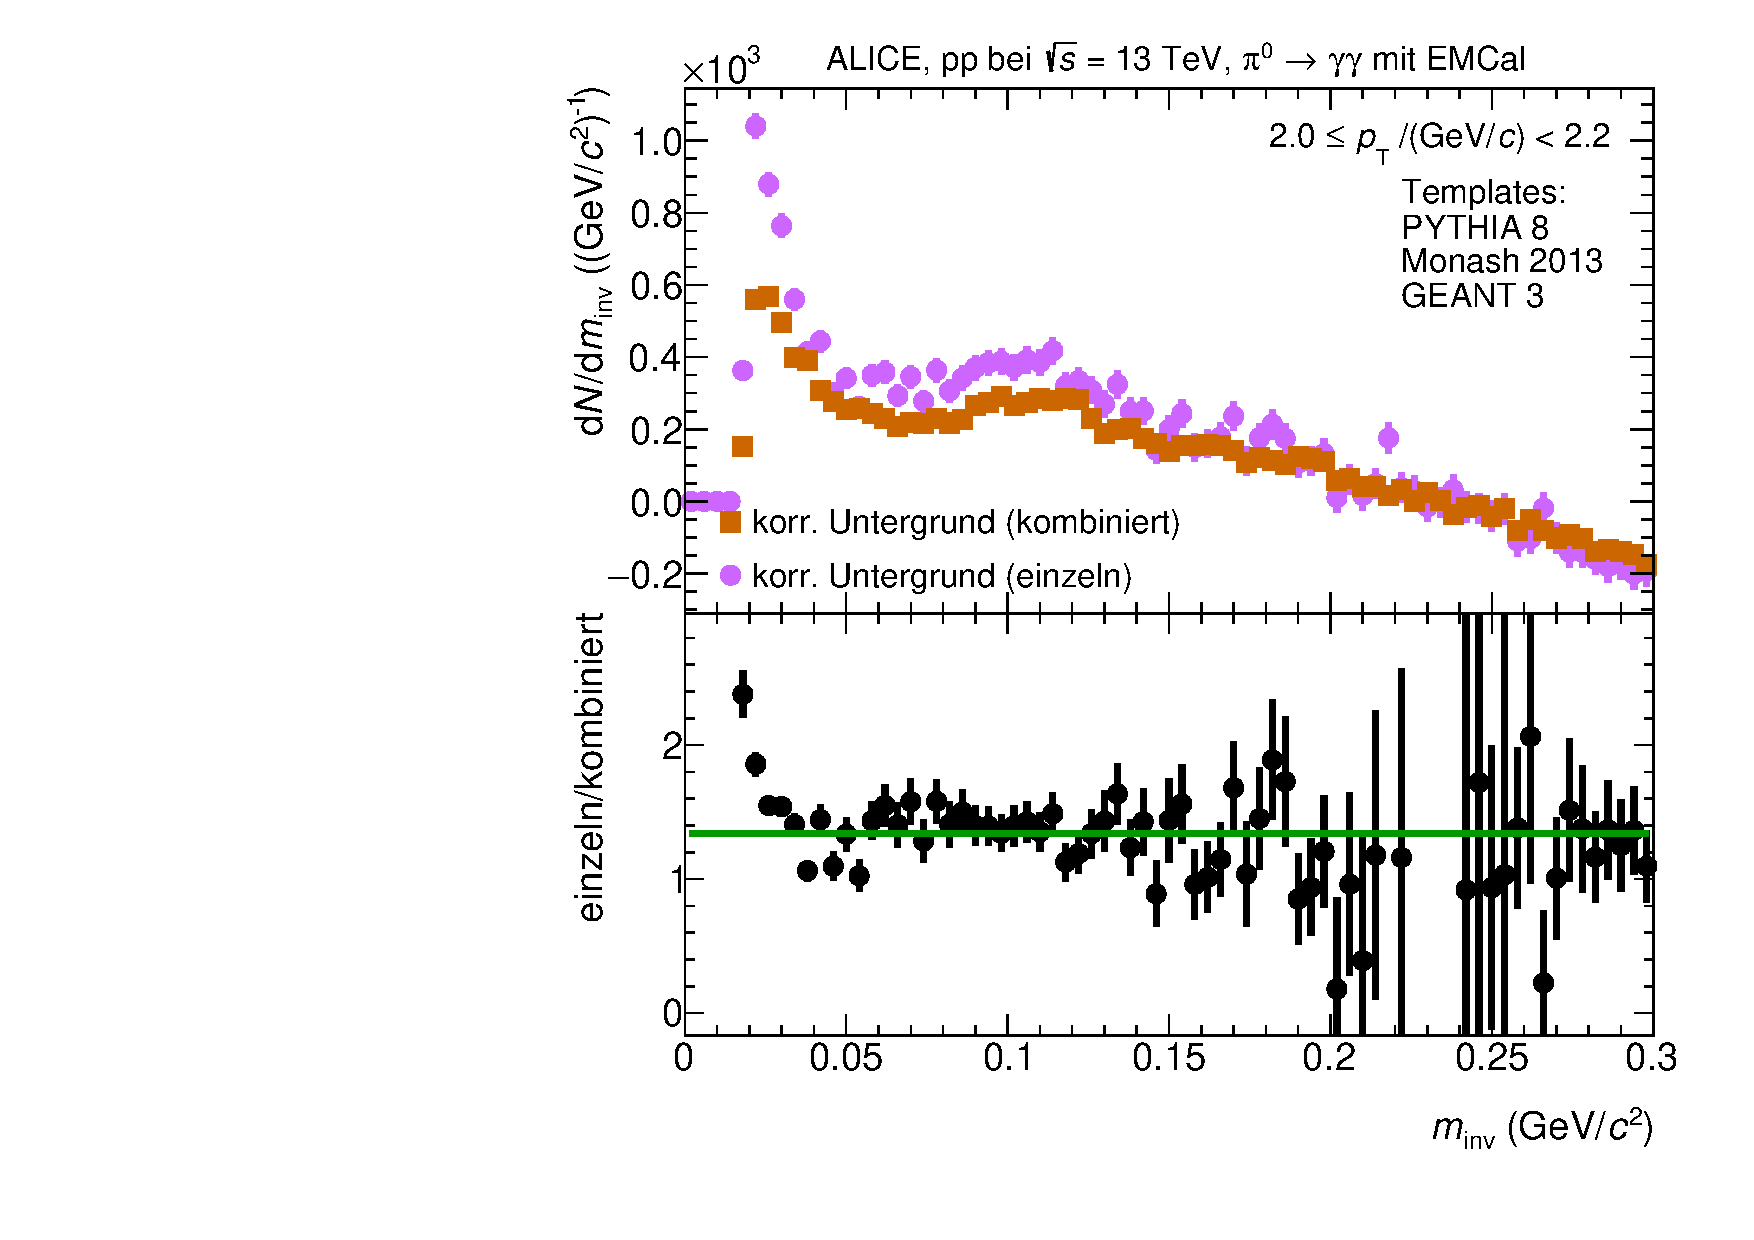
\includegraphics[width=.65\linewidth]{Anhang/BackgroundWithRatio04_Data_2016.pdf}\par
\end{multicols}
\begin{multicols}{2}
    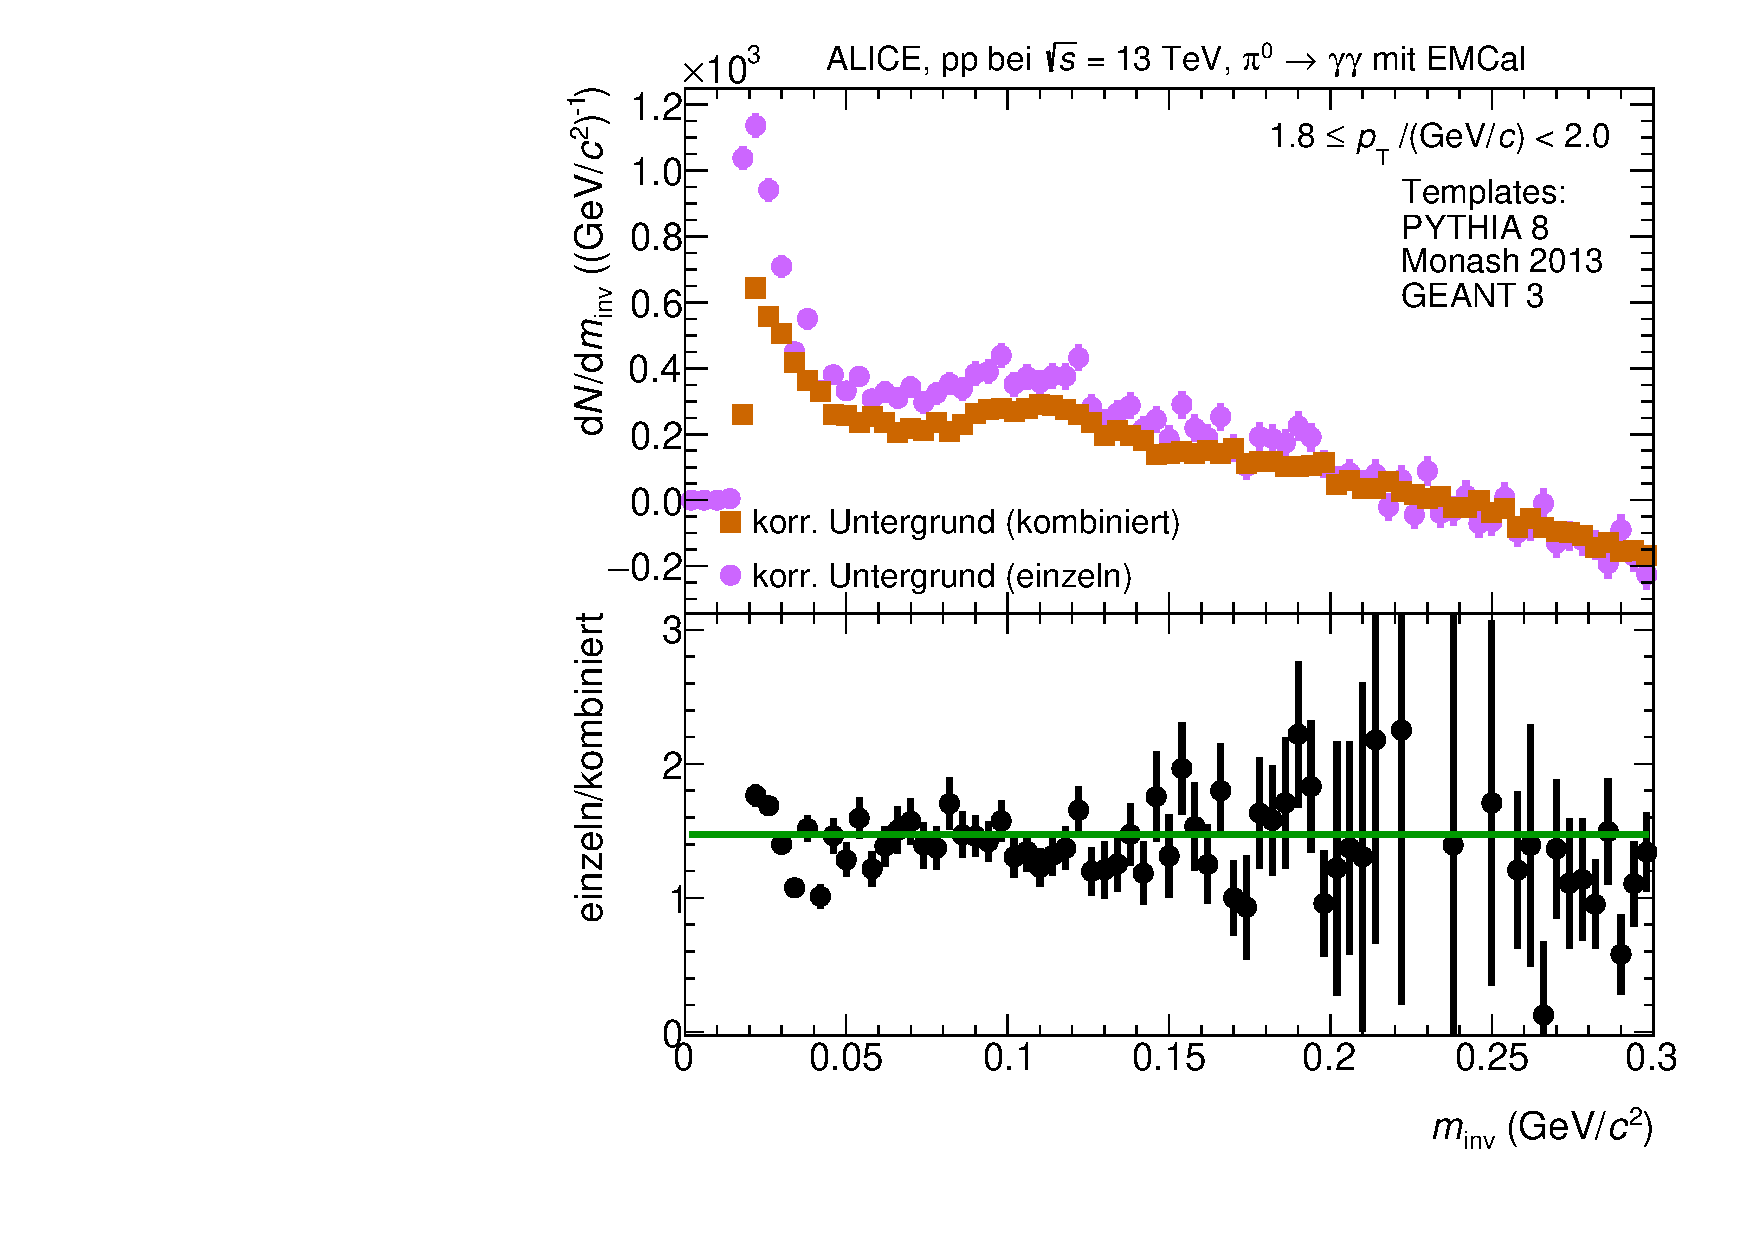
\includegraphics[width=.65\linewidth]{Anhang/BackgroundWithRatio03_Data_2016.pdf}\par
    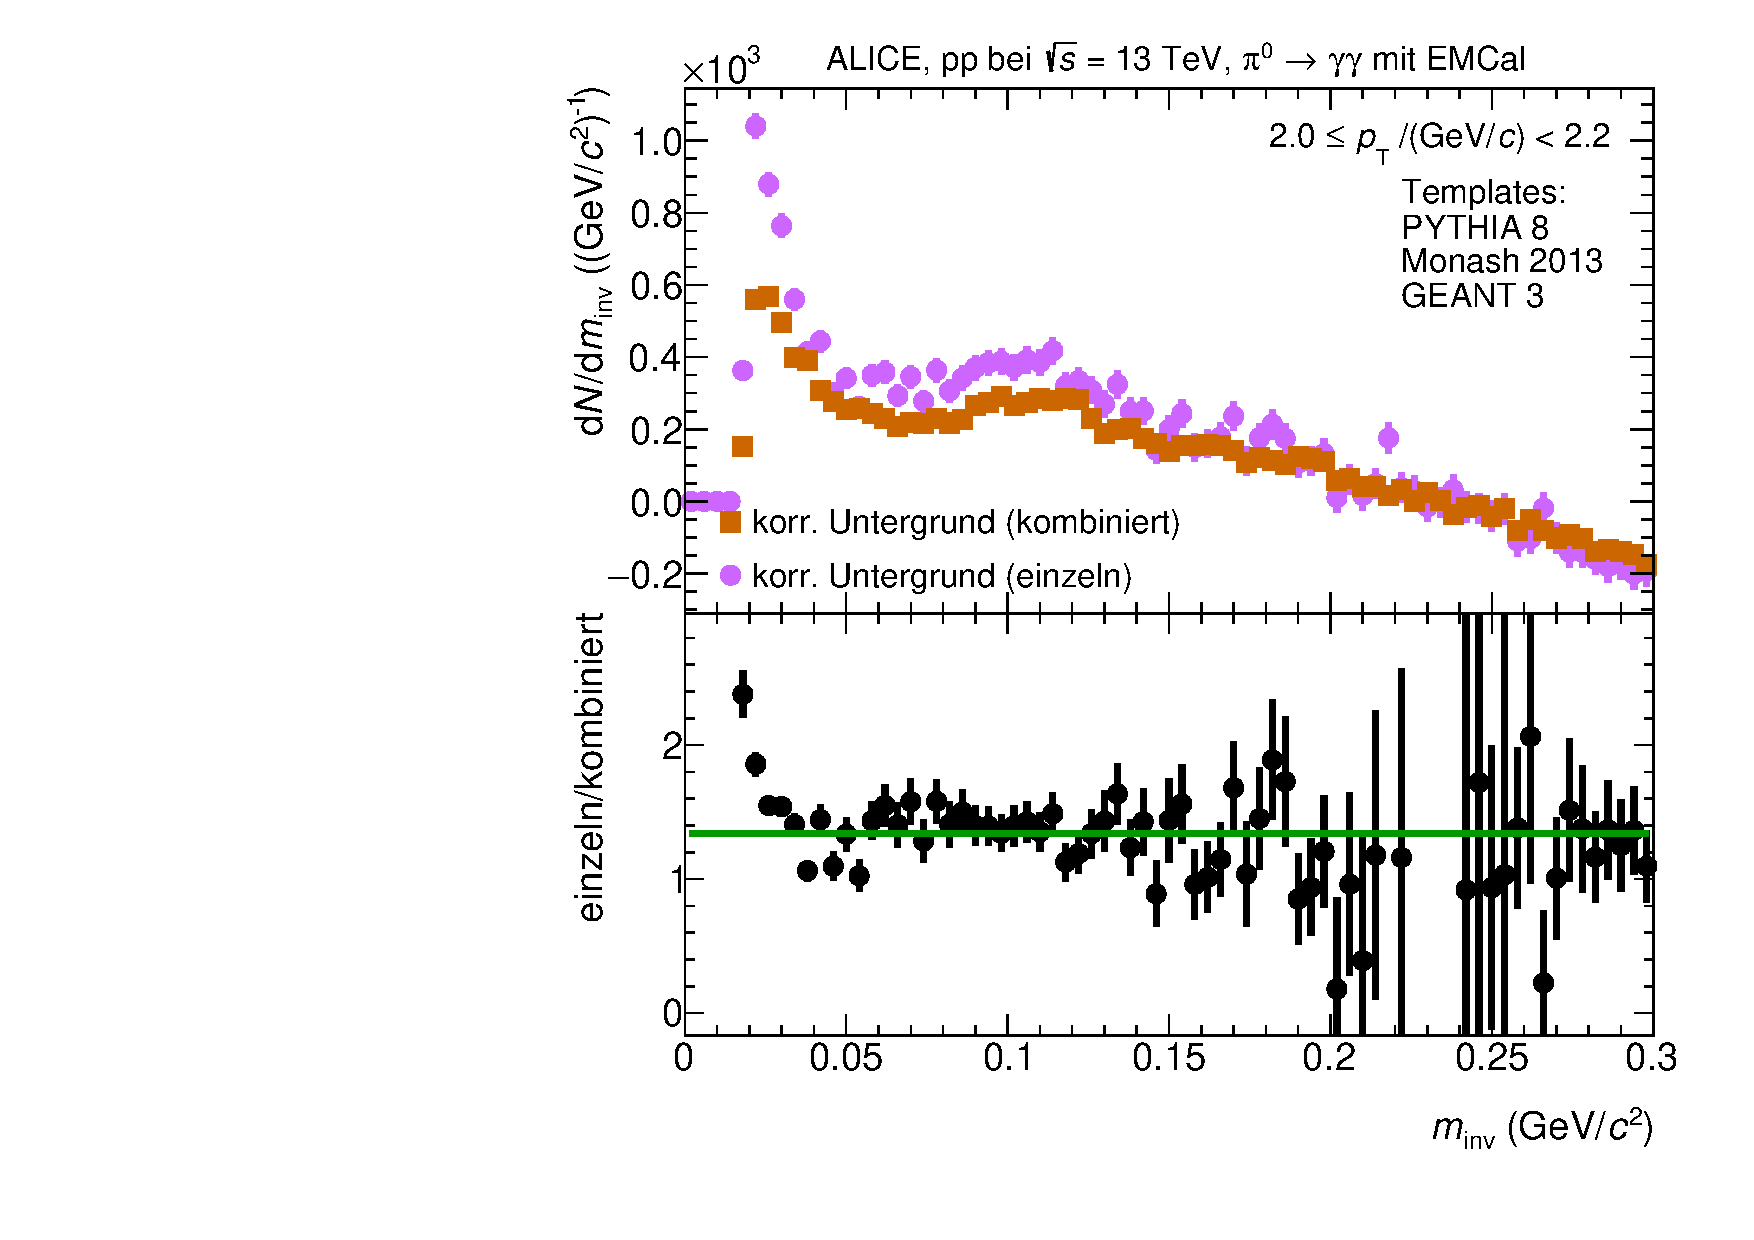
\includegraphics[width=.65\linewidth]{Anhang/BackgroundWithRatio04_Data_2016.pdf}\par
\end{multicols}
\begin{multicols}{2}
    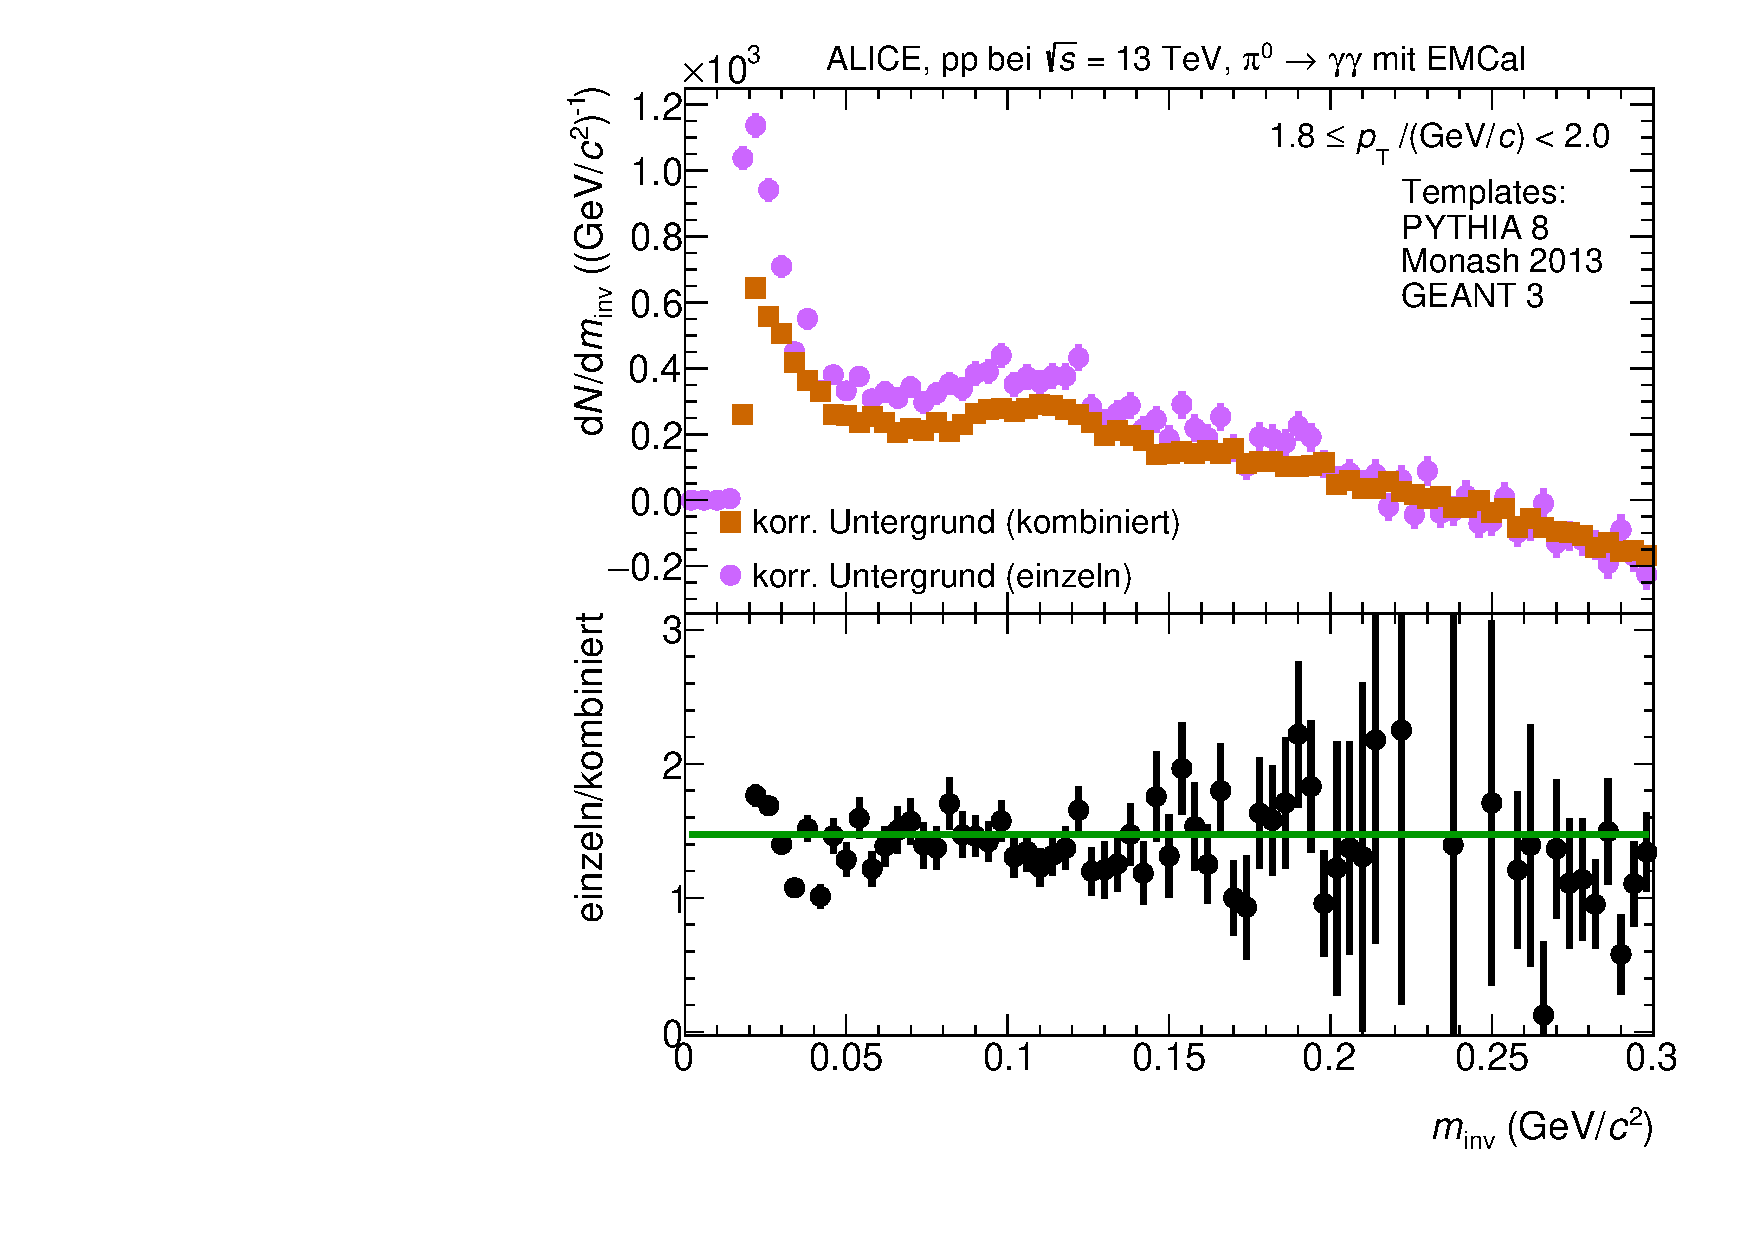
\includegraphics[width=.65\linewidth]{Anhang/BackgroundWithRatio03_Data_2016.pdf}\par
    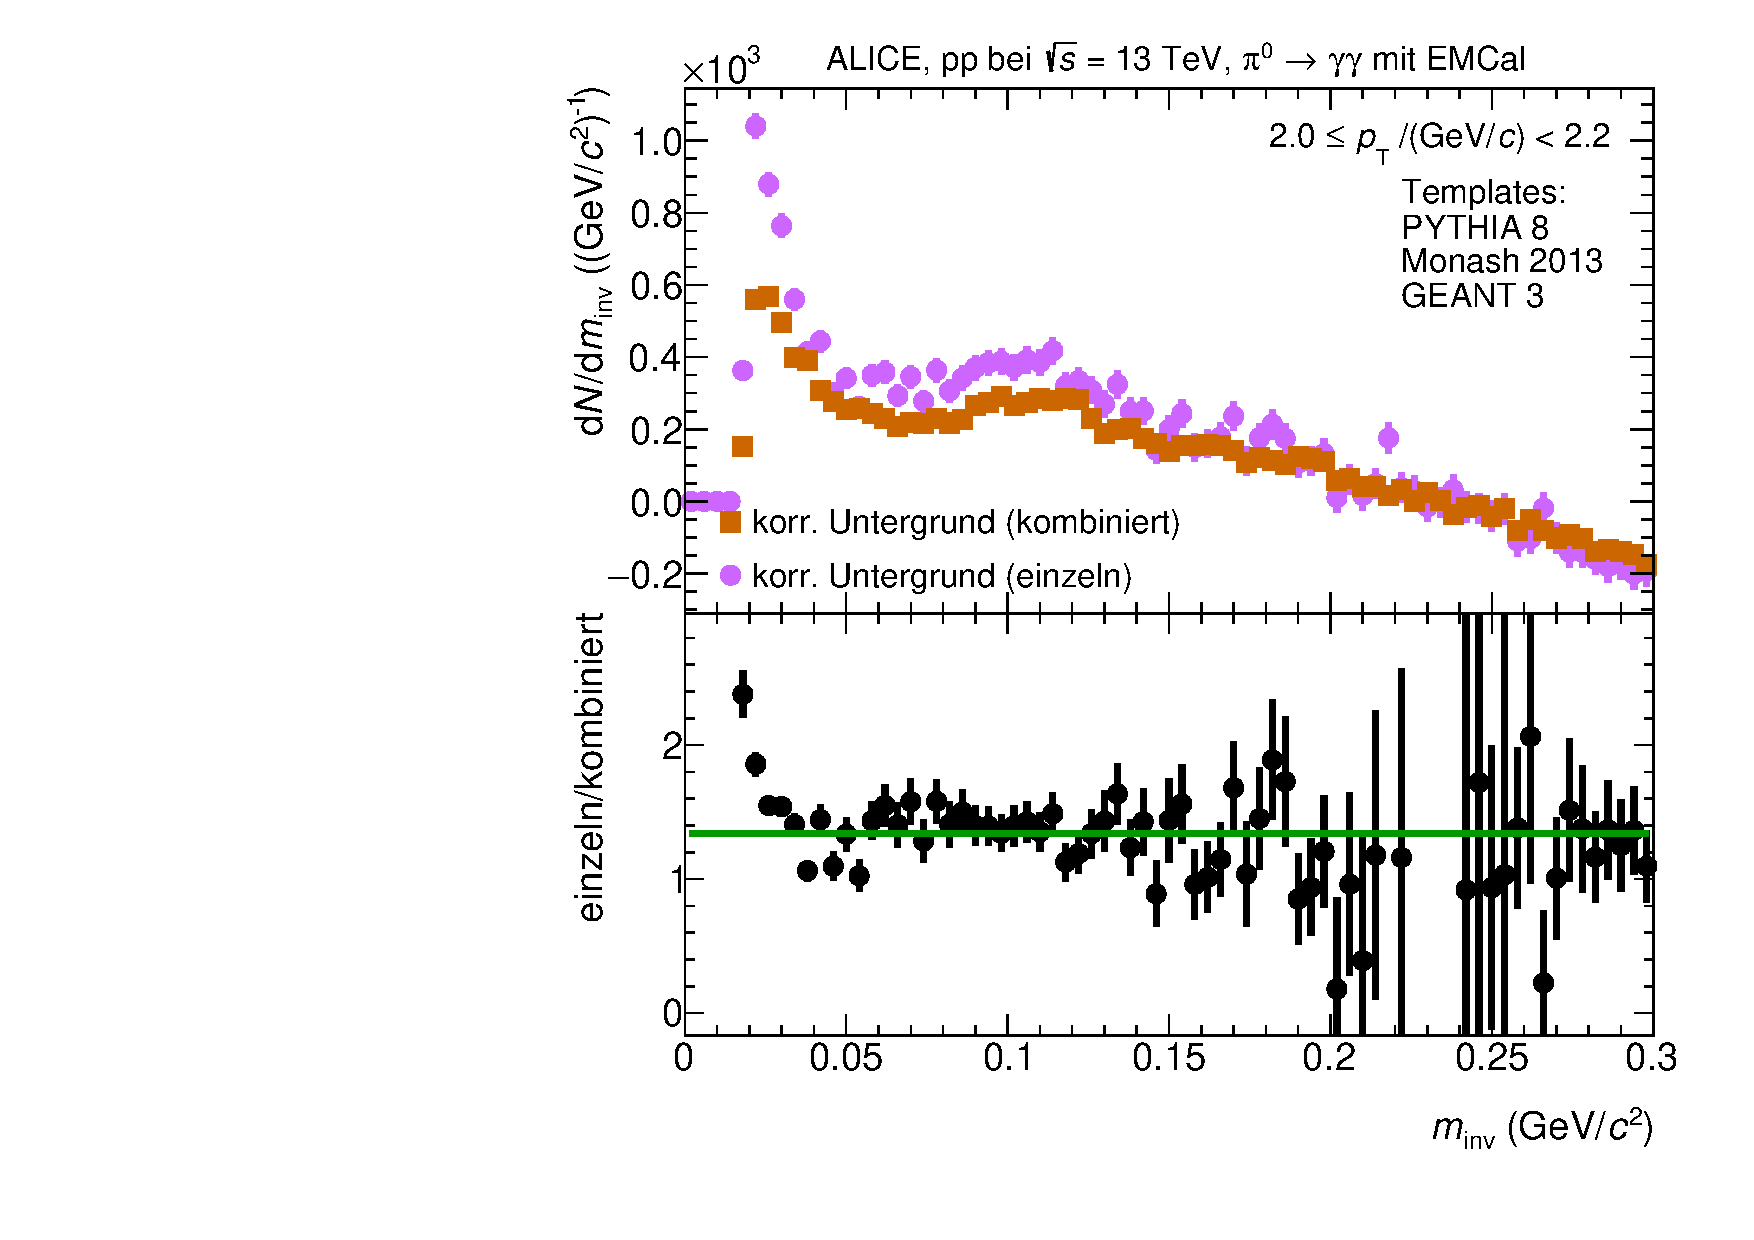
\includegraphics[width=.65\linewidth]{Anhang/BackgroundWithRatio04_Data_2016.pdf}\par
\end{multicols}
\end{figure*}
\clearpage

\begin{figure*}[t!]
\begin{multicols}{2}
	\centering
    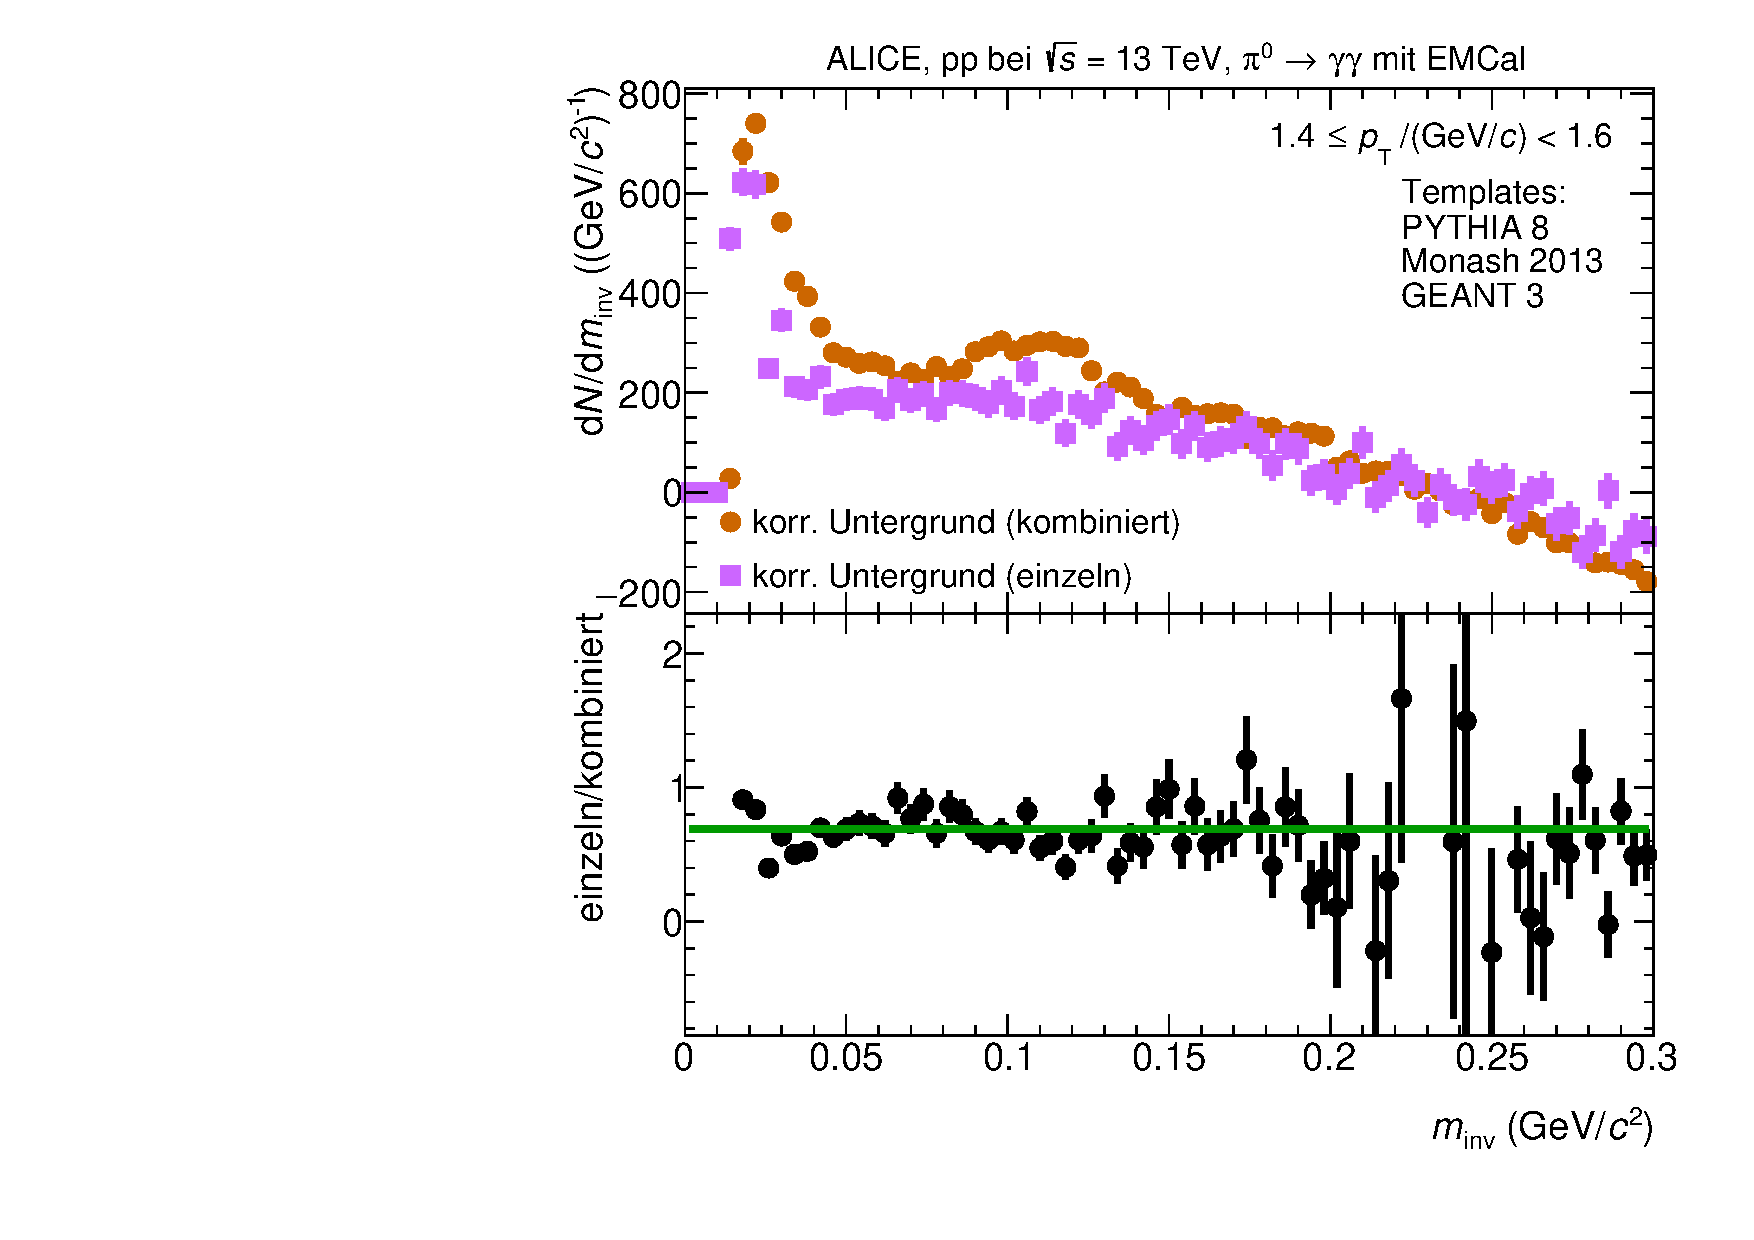
\includegraphics[width=.65\linewidth]{Anhang/BackgroundWithRatio01_Data_2016.pdf}\par 
    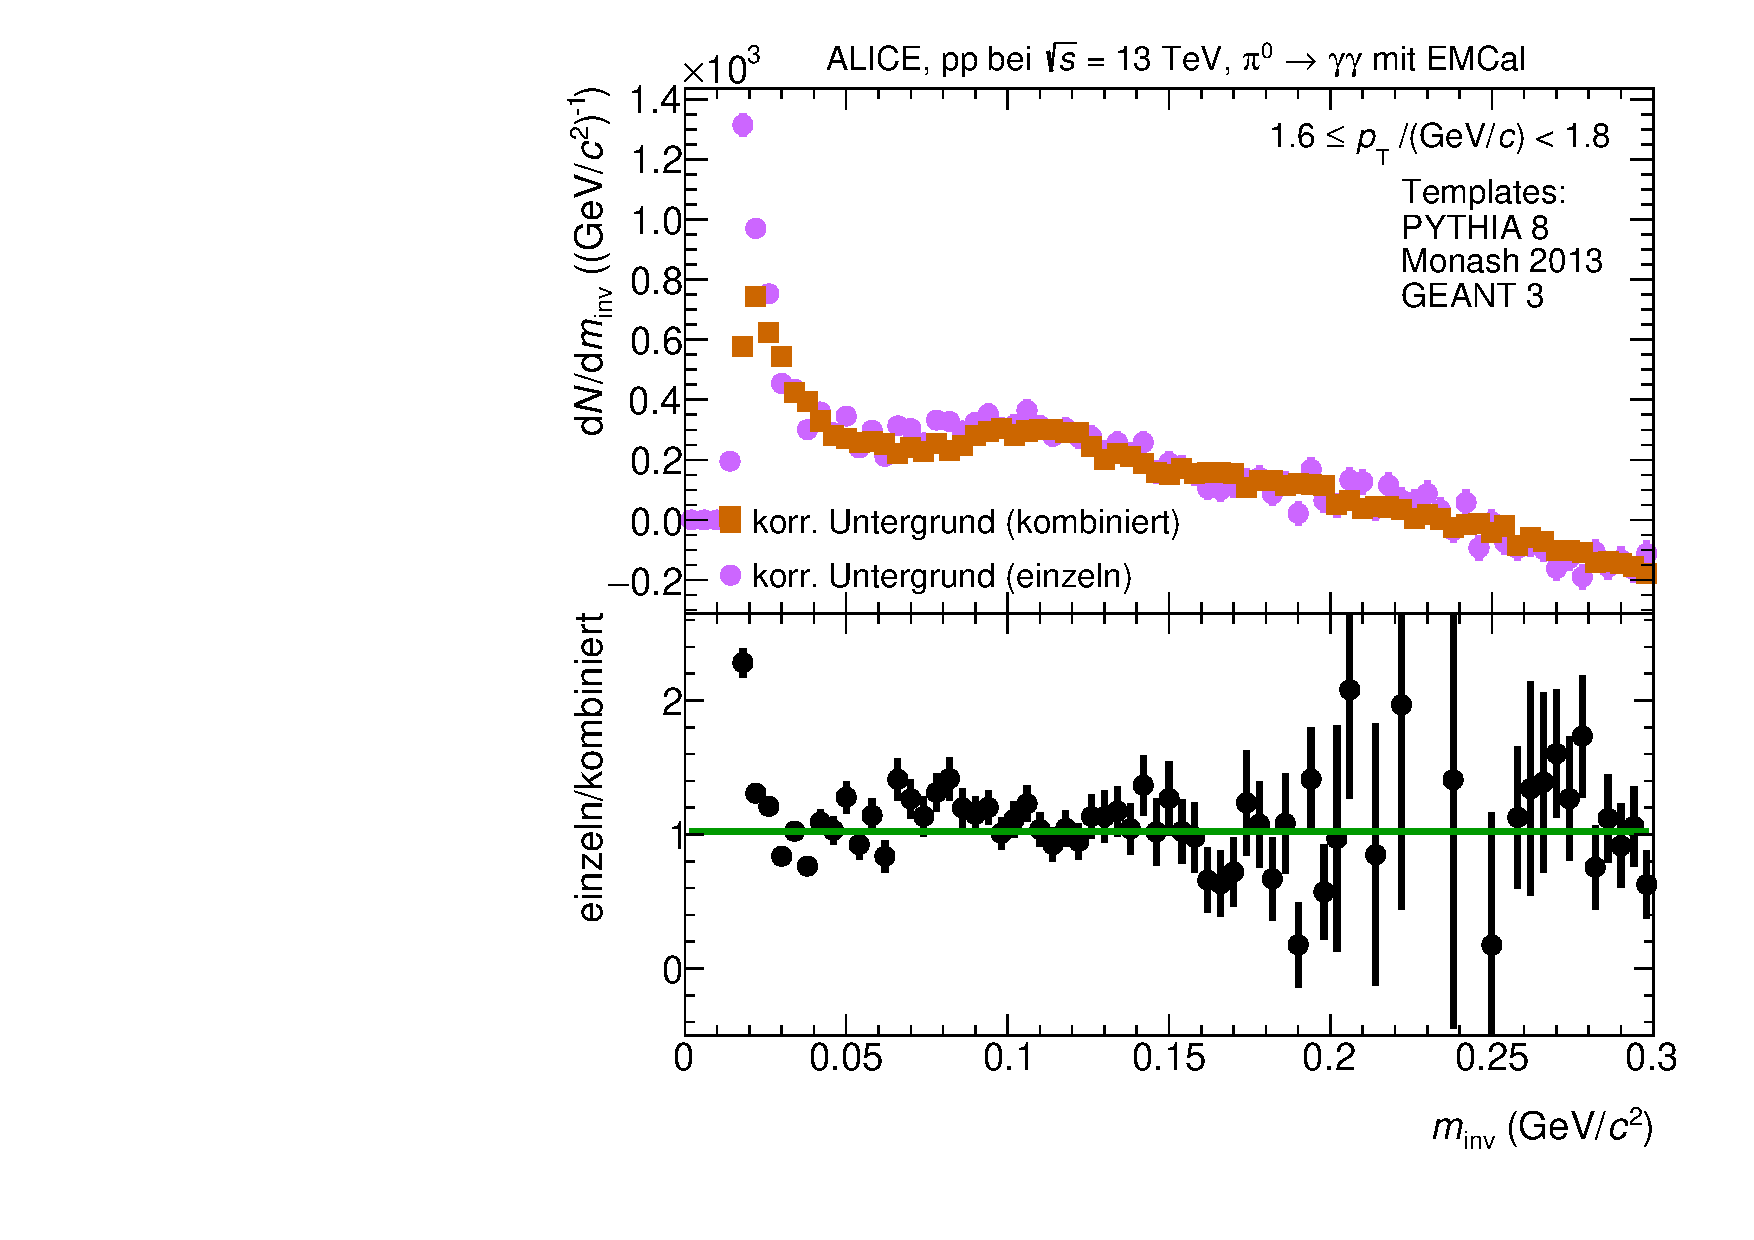
\includegraphics[width=.65\linewidth]{Anhang/BackgroundWithRatio02_Data_2016.pdf}\par 
\end{multicols}
\caption{Vergleich der Templates des korrelierten Untergrunds aus den restlichen $p_\text{T}$-Intervallen mit dem kombinierten Template des korrelierten Untergrunds.}
\label{fig:OtherRatios}
\end{figure*}
\clearpage


%\begin{figure}
%\begin{subfigure}{.5\textwidth}
%  \centering
%  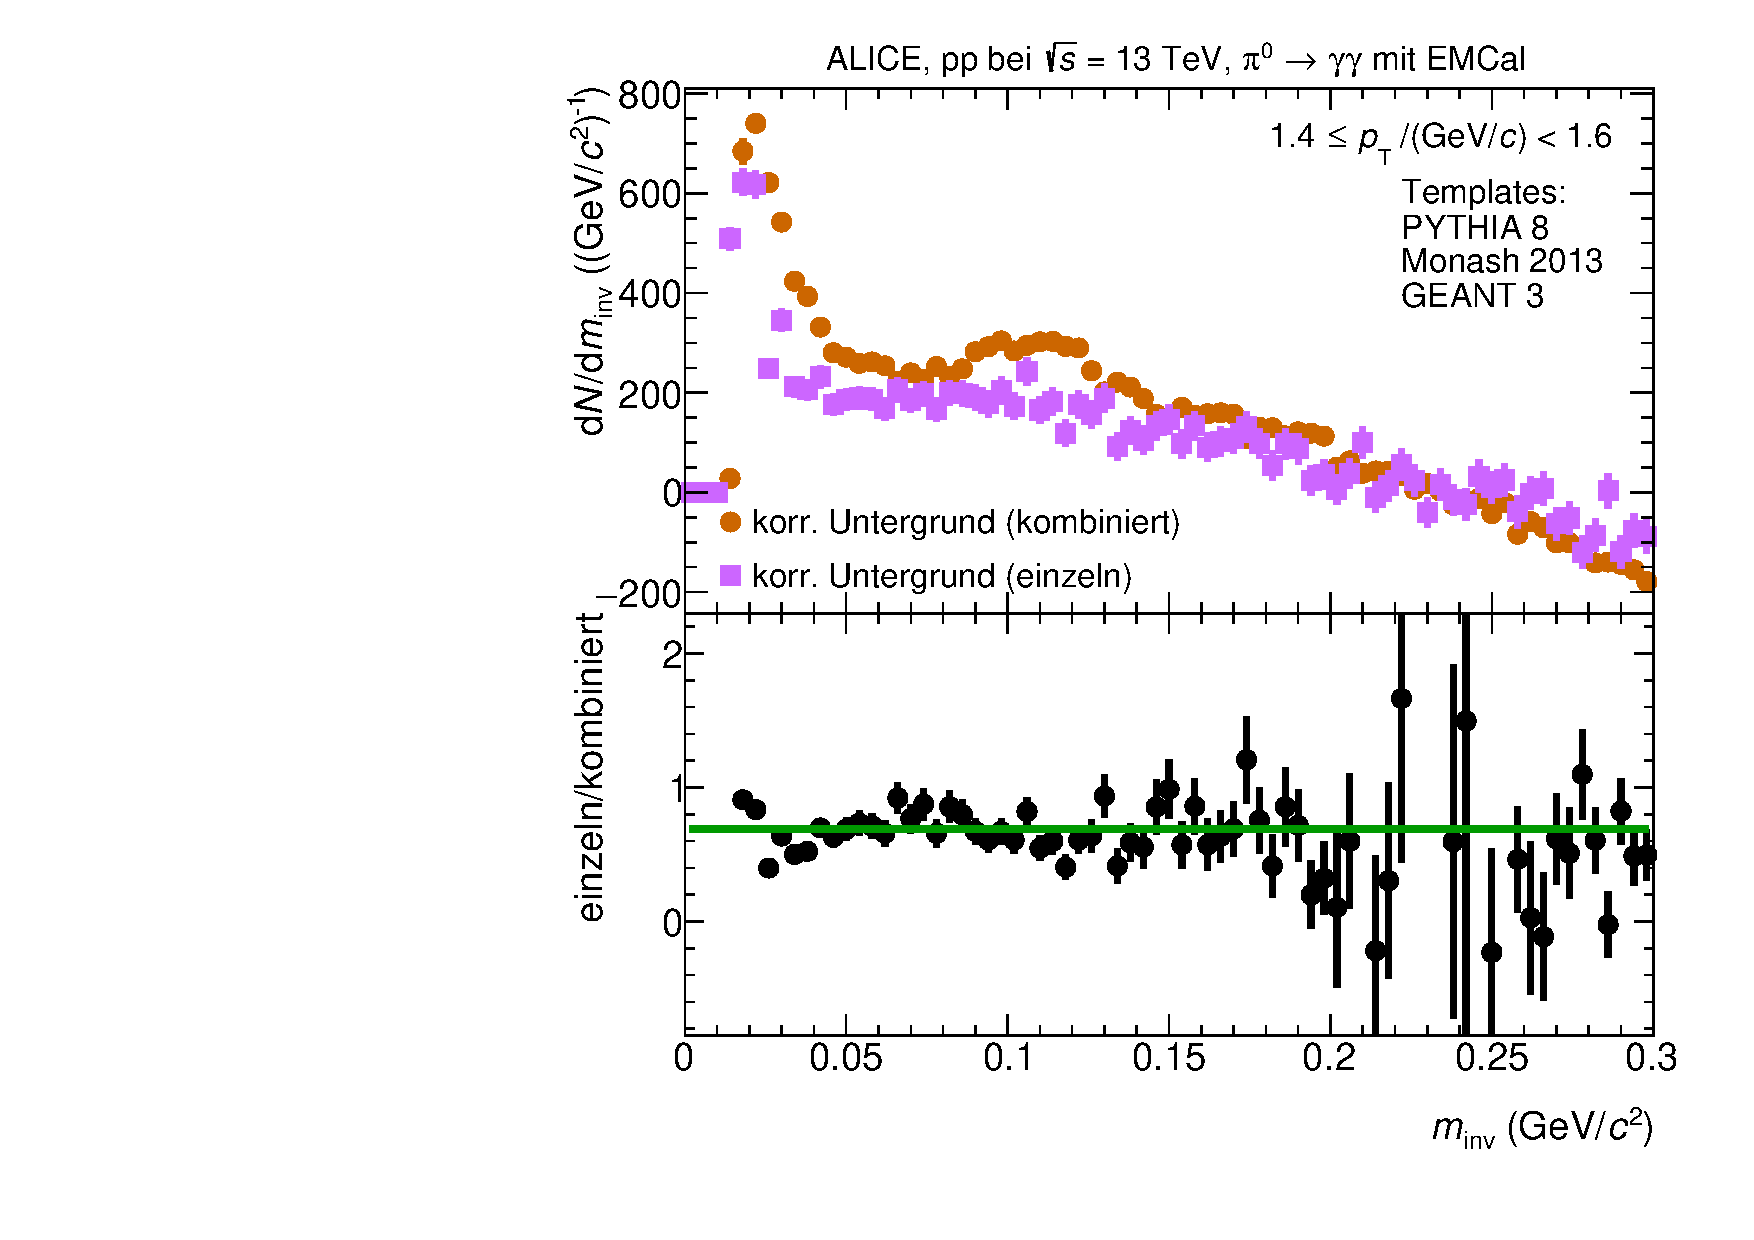
\includegraphics[width=.8\linewidth]{Anhang/BackgroundWithRatio01_Data_2016.pdf}
%\end{subfigure}%
%\begin{subfigure}{.5\textwidth}
%  \centering
%  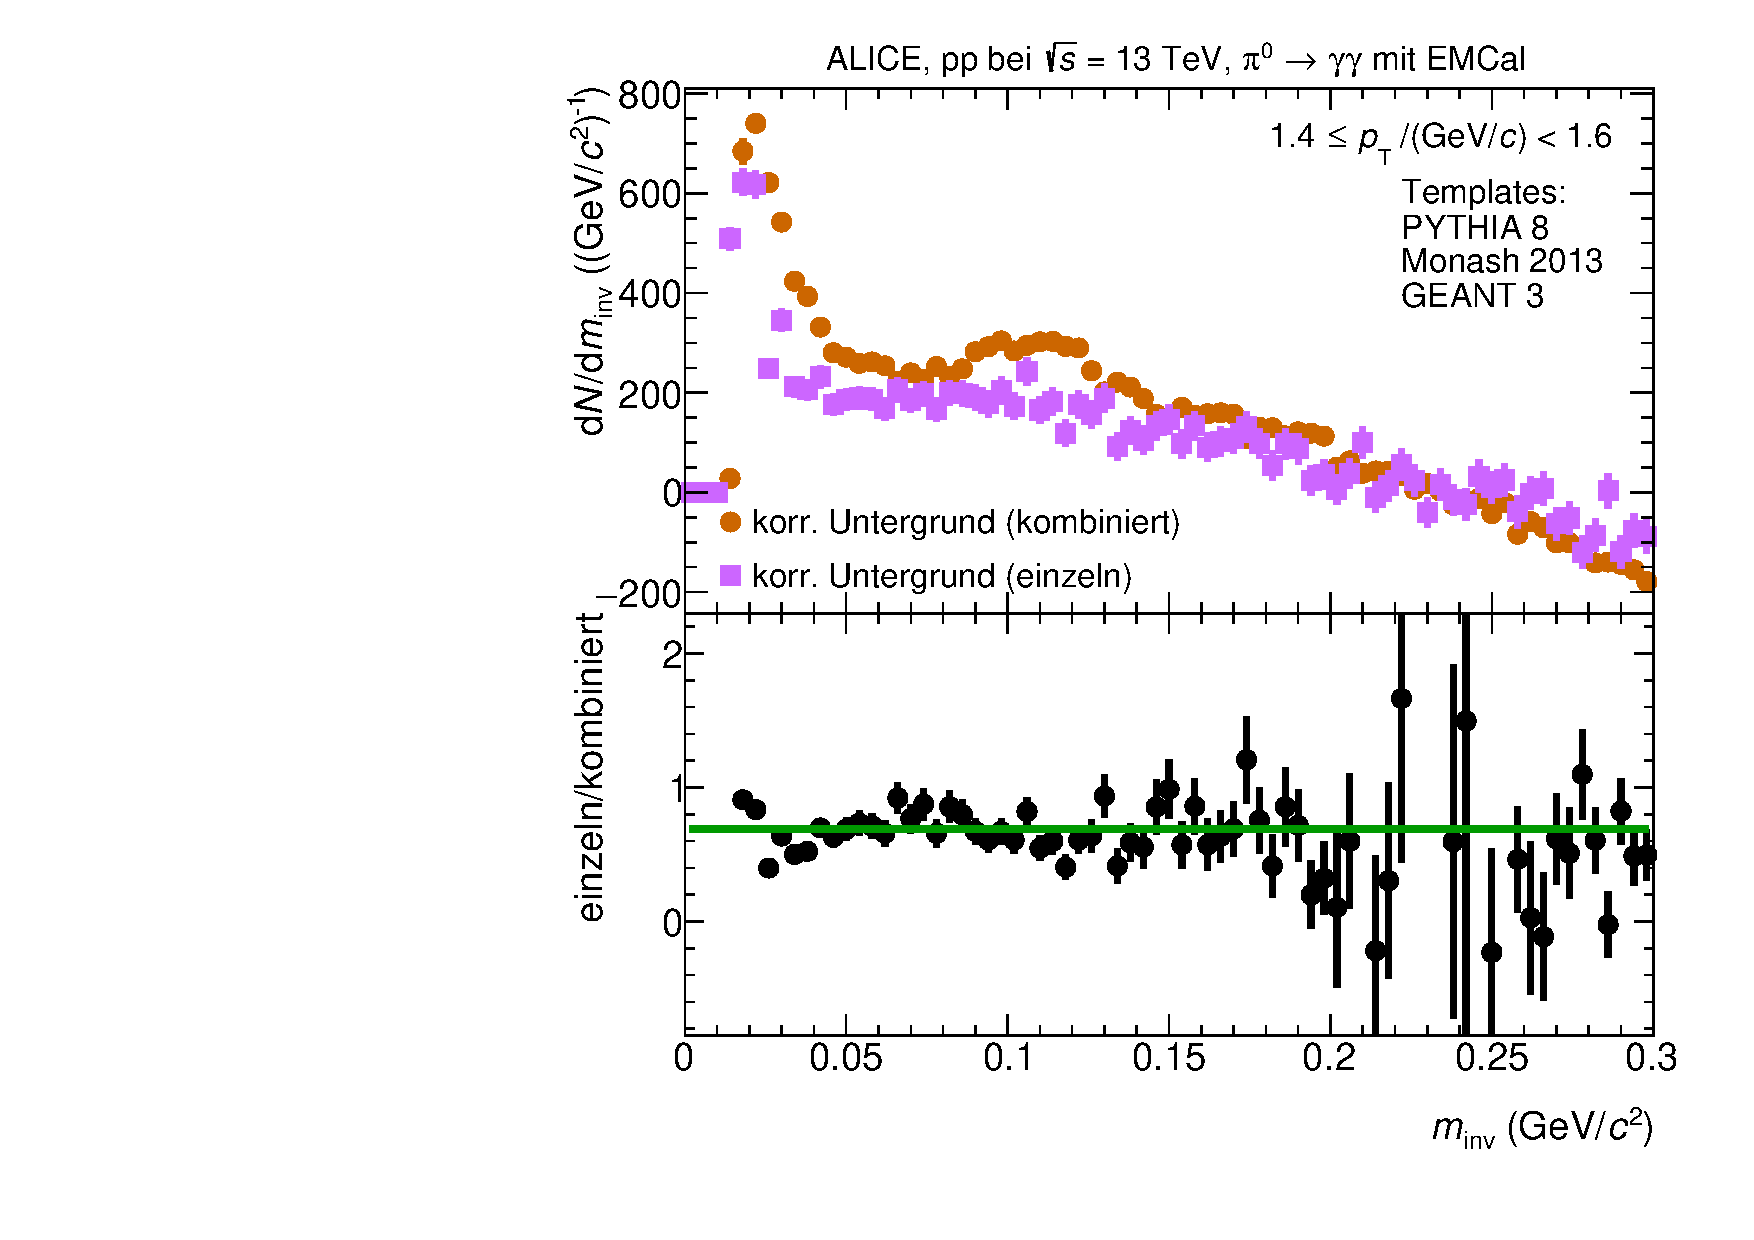
\includegraphics[width=.8\linewidth]{Anhang/BackgroundWithRatio01_Data_2016.pdf}
%\end{subfigure}
%\caption{plots of something}
%\label{fig:fig}
%\end{figure}